%%
%% This is file `sample-sigconf.tex',
%% generated with the docstrip utility.
%%
%% The original source files were:
%%
%% samples.dtx  (with options: `sigconf')
%% 
%% IMPORTANT NOTICE:
%% 
%% For the copyright see the source file.
%% 
%% Any modified versions of this file must be renamed
%% with new filenames distinct from sample-sigconf.tex.
%% 
%% For distribution of the original source see the terms
%% for copying and modification in the file samples.dtx.
%% 
%% This generated file may be distributed as long as the
%% original source files, as listed above, are part of the
%% same distribution. (The sources need not necessarily be
%% in the same archive or directory.)
%%
%%%% Proceedings format for most of ACM conferences (with the exceptions listed below) and all ICPS volumes.
\documentclass[sigconf, anonymous]{acmart}
\usepackage{cleveref}
\usepackage{graphicx}
\usepackage{subfigure}
\usepackage{threeparttable}
\usepackage{enumitem}
\usepackage{bigstrut,multirow}
\usepackage{algorithm}  
\usepackage{algorithmicx}  
\usepackage{algpseudocode}  
\usepackage{amsmath} 
\usepackage{lipsum}
\usepackage{array}
\usepackage{float}
\usepackage{stfloats}
% \floatname{algorithm}{ROSExample} 
%%%% As of March 2017, [siggraph] is no longer used. Please use sigconf (above) for SIGGRAPH conferences.

%%%% Proceedings format for SIGPLAN conferences 
% \documentclass[sigplan, anonymous, review]{acmart}

%%%% Proceedings format for SIGCHI conferences
% \documentclass[sigchi, review]{acmart}

%%%% To use the SIGCHI extended abstract template, please visit
% https://www.overleaf.com/read/zzzfqvkmrfzn

%%
%% \BibTeX command to typeset BibTeX logo in the docs
% \AtBeginDocument{%
%   \providecommand\BibTeX{{%
%     \normalfont B\kern-0.5em{\scshape i\kern-0.25em b}\kern-0.8em\TeX}}}

%% Rights management information.  This information is sent to you
%% when you complete the rights form.  These commands have SAMPLE
%% values in them; it is your responsibility as an author to replace
%% the commands and values with those provided to you when you
%% complete the rights form.
% \copyrightyear{2019}
% \acmYear{2019}
% \setcopyright{rightsretained}

%% These commands are for a PROCEEDINGS abstract or paper.
% \acmConference{SIGGRAPH '19 Talks}{July 28 - August 01, 2019}{Los Angeles, CA, USA}
% \acmDOI{10.1145/3306307.3328180}
% \acmISBN{978-1-4503-6317-4/19/07}
% \acmBooktitle{SIGGRAPH '19 Talks, 
%   July 28 - August 01, 2019, Los Angeles, CA}


%%
%% Submission ID.
%% Use this when submitting an article to a sponsored event. You'll
%% receive a unique submission ID from the organizers
%% of the event, and this ID should be used as the parameter to this command.
%%\acmSubmissionID{123-A56-BU3}
 
%%
%% The majority of ACM publications use numbered citations and
%% references.  The command \citestyle{authoryear} switches to the
%% "author year" style.
%%
%% If you are preparing content for an event
%% sponsored by ACM SIGGRAPH, you must use the "author year" style of
%% citations and references.
%% Uncommenting
%% the next command will enable that style.
%%\citestyle{acmauthoryear}

%%
%% end of the preamble, start of the body of the document source.


\settopmatter{printacmref=false} % Removes citation information below abstract
\renewcommand\footnotetextcopyrightpermission[1]{} % removes footnote with conference information in first column
\pagestyle{plain} % removes running headers

\begin{document}

%%
%% The "title" command has an optional parameter,
%% allowing the author to define a "short title" to be used in page headers.
% \title{MUROEXE : A Multi-Agent Exploration Engine Based on Interruptible CNN Accelerator on Embedded FPGA}
\title{INCAME : INterruptible CNN Accelerator for Multi-robot Exploration}

%%
%% The "author" command and its associated commands are used to define
%% the authors and their affiliations.
%% Of note is the shared affiliation of the first two authors, and the
%% "authornote" and "authornotemark" commands
%% used to denote shared contribution to the research.
\author{Jincheng Yu}
% \authornote{Both authors contributed equally to this research.}

%%
%% By default, the full list of authors will be used in the page
%% headers. Often, this list is too long, and will overlap
%% other information printed in the page headers. This command allows
%% the author to define a more concise list
%% of authors' names for this purpose.
% \renewcommand{\shortauthors}{Trovato and Tobin, et al.}

%%
%% The abstract is a short summary of the work to be presented in the
%% article.
\begin{abstract}
% Multi-Robot Exploration (MR-Exploration) that provides the location and map is the basic task for many multi-robot applications. 
% With the development of Convolutional Neural Network (CNN), the accuracy of some critical components in MR-Exploration, such as Feature-point Extraction (FE) and Place Recognition (PR), can significantly benefit from CNN. 
% To deploy CNN on the embedded real-time system, previous works design CNN accelerators on FPGA. 
% However, these accelerators mainly focus on improving the performance of a single network, lacking support for multi-task. 
% Since researchers in robotic usually run different CNN tasks simultaneously, the inability of accelerators to support multi-task makes it difficult for researchers in robotic to use embedded FPGA. 
% Furthermore, the post-processing of  CNN-based components (such as FE and PR), which is also computation consuming, becomes the bottleneck of the system, after accelerating the CNN backbones.

Multi-Robot Exploration (MR-Exploration) that provides the location and map is a basic task for many multi-robot applications. Recent researches introduce Convolutional Neural Network (CNN) to critical components in MR-Exploration, like Feature-point Extraction (FE) and Place Recognition (PR), to improve the system performance. Such CNN-based MR-Exploration requires running multiple CNN models simultaneously, together with complex post-processing algorithms, greatly challenges the hardware platforms, which are usually embedded systems.
Previous researches have shown that FPGA is a good candidate for CNN processing on embedded platforms. But such accelerators usually process different models sequentially, lacking the ability to schedule multiple tasks at runtime. Furthermore, post-processing of CNNs in FE is also computation consuming and becomes the system bottleneck after accelerating the CNN models.

To handle such problems, we propose an INterruptible CNN Accelerator for Multi-Robot Exploration (INCAME) framework for rapid deployment of robot applications on FPGA. In INCAME, we propose a virtual-instruction-based interrupt method to support multi-task on CNN accelerators. INCAME also includes hardware modules to accelerate the post-processing of the CNN-based components.
Experimental results show that INCAME enables multi-task scheduling on the CNN accelerator with negligible performance degradation (0.3\%). With the help of multi-task supporting and post-processing acceleration, INCAME enables embedded FPGA to execute MR-Exploration in real time (20 fps).

% To handle such problems, we propose an INterruptible CNN Accelerator for Multi-Robot Exploration (INCAME) framework for rapid deployment of MR-Exploration on FPGA.
% In INCAME, we propose a virtual-instruction-based interrupt method to support multi-task on CNN accelerators.
% INCAME also includes hardware modules to accelerate the post-processing of the CNN-based components.
% % We evaluate INCAME on Xilinx ZU9 MPSoC. 
% The experiment results show that INCAME enables multi-task scheduling on the CNN accelerator with negligible performance reduction (0.8\%). With the help of multi-task supporting and post-processing accelerating, INCAME enables embedded FPGA to execute MR-Exploration in real time (20 fps).
% Multi-Robot Exploration (MR-Exploration) that provides the location and maps is the basic task for many multi-robot applications. 
% Feature-point Extraction (FE) and Place Recognition (PR) are two critical modules in MR-Exploration.
% The accuracy of both modules can benefit from Convolutional Neural Network (CNN).
% Previous CNN accelerators on FPGA mainly focus on improving the performance of a single neural network, lacking multi-task support.
% Researchers in robotic usually run several CNN tasks simultaneously, such as FE and PR.
% The inability of CNN accelerators to support multi-task makes it difficult for researchers in robotic to use embedded FPGA.

% We propose a \textit{MU}lti-\textit{RO}bot \textit{EX}ploration \textit{E}ngine (MUROEXE) to deploy MR-Exploration on embedded FPGA. 
% We propose a virtual-instruction-based interrupt method to support multi-task on CNN accelerators.
% Besides the CNN backbone, the post-precessing for CNN-based FE and PR is also computation consuming. 
% MUROEXE introduces RTL/HLS modules to accelerate the post-precessing of CNN-based modules.
% Experiments show that MUROEXE supports multi-thread scheduling with negligible performance reduction (??\%).
% MUROEXE enables embedded FPGA (Xilinx ZU9) executing MR-Exploration in real-time (30 fps).
\end{abstract}

%%
%% The code below is generated by the tool at http://dl.acm.org/ccs.cfm.
%% Please copy and paste the code instead of the example below.
%%
% \begin{CCSXML}
% <ccs2012>
%  <concept>
%   <concept_id>10010520.10010553.10010562</concept_id>
%   <concept_desc>Computer systems organization~Embedded systems</concept_desc>
%   <concept_significance>500</concept_significance>
%  </concept>
%  <concept>
%   <concept_id>10010520.10010575.10010755</concept_id>
%   <concept_desc>Computer systems organization~Redundancy</concept_desc>
%   <concept_significance>300</concept_significance>
%  </concept>
%  <concept>
%   <concept_id>10010520.10010553.10010554</concept_id>
%   <concept_desc>Computer systems organization~Robotics</concept_desc>
%   <concept_significance>100</concept_significance>
%  </concept>
%  <concept>
%   <concept_id>10003033.10003083.10003095</concept_id>
%   <concept_desc>Networks~Network reliability</concept_desc>
%   <concept_significance>100</concept_significance>
%  </concept>
% </ccs2012>
% \end{CCSXML}

% \ccsdesc[500]{Computer systems organization~Embedded systems}
% \ccsdesc[300]{Computer systems organization~Redundancy}
% \ccsdesc{Computer systems organization~Robotics}
% \ccsdesc[100]{Networks~Network reliability}

%%
%% Keywords. The author(s) should pick words that accurately describe
%% the work being presented. Separate the keywords with commas.
% \keywords{FPGA, CNN accelerator, Multi-Robot}


%%
%% This command processes the author and affiliation and title
%% information and builds the first part of the formatted document.
\maketitle

\section{INTRODUCTION}
\label{sec:intro}

The cooperation of agents can expand the capability of the unmanned system, and the multi-agent intelligent system is a promising research field.
Multi-Robot Exploration (MR-Exploration)  ~\cite{corah2019communication} provides location and map for each robot, and is the basic task for many multi-robot applications, such as multi-robot navigation  ~\cite{tanner2005towards} and multi-robot rescue  ~\cite{baxter2007multi}.

The  MR-Exploration system  ~\cite{corah2019communication, cieslewski2018data} consists of several robots, each of which executes the system illustrated in \Cref{fig:maexp}. Each input frame is fed to the Feature-point Extraction (FE, \textcircled{1}) module for Visual Odometry (VO). 
And some input frames, called key frames, are fed to the Place Recognition (PR, \textcircled{2}) module.
PR module generates the compact image representation, which produces the candidate place recognition matches between different robots. The Visual Odometry (VO) (\textcircled{3}) matches the the feature-points of two adjacent frames to produce the 6 Degrees of Freedom (6-DoF) poses. Based on the 6-DoF poses,  map and the trajectory can be used for location. The relative pose (RelPose) module does the same operation as VO(\textcircled{3}) and establishes relative poses between the candidate place matches. The decentralized optimization module (DOpt, \textcircled{4}) and the global map generation module (\textcircled{5}) optimize the intra-robot relative pose measurements from VO and the inter-robot relative pose measurements from RelPose, and merge the maps. The exploration module (\textcircled{6}) decides an unexplored goal point for each robot to move based on the merged map and the estimated location. The navigation module (\textcircled{7}) guides each robot to the goal point, including path planning and obstacle avoidance.
In this paper, we optimize the scheduling of PR(\textcircled{2}) and the VO (\textcircled{3}) based on the feature-points (\textcircled{1}), across the CPU side (processing system, PS) and FPGA side (programmable logic, PL), on Xilinx MPSoC  ~\cite{MPSoC}.

\begin{figure}[t]
    \centering
    % \vspace{-0.1cm} 
    % \setlength{\abovecaptionskip}{0cm} 
    % \setlength{\belowcaptionskip}{-0.4cm} 
	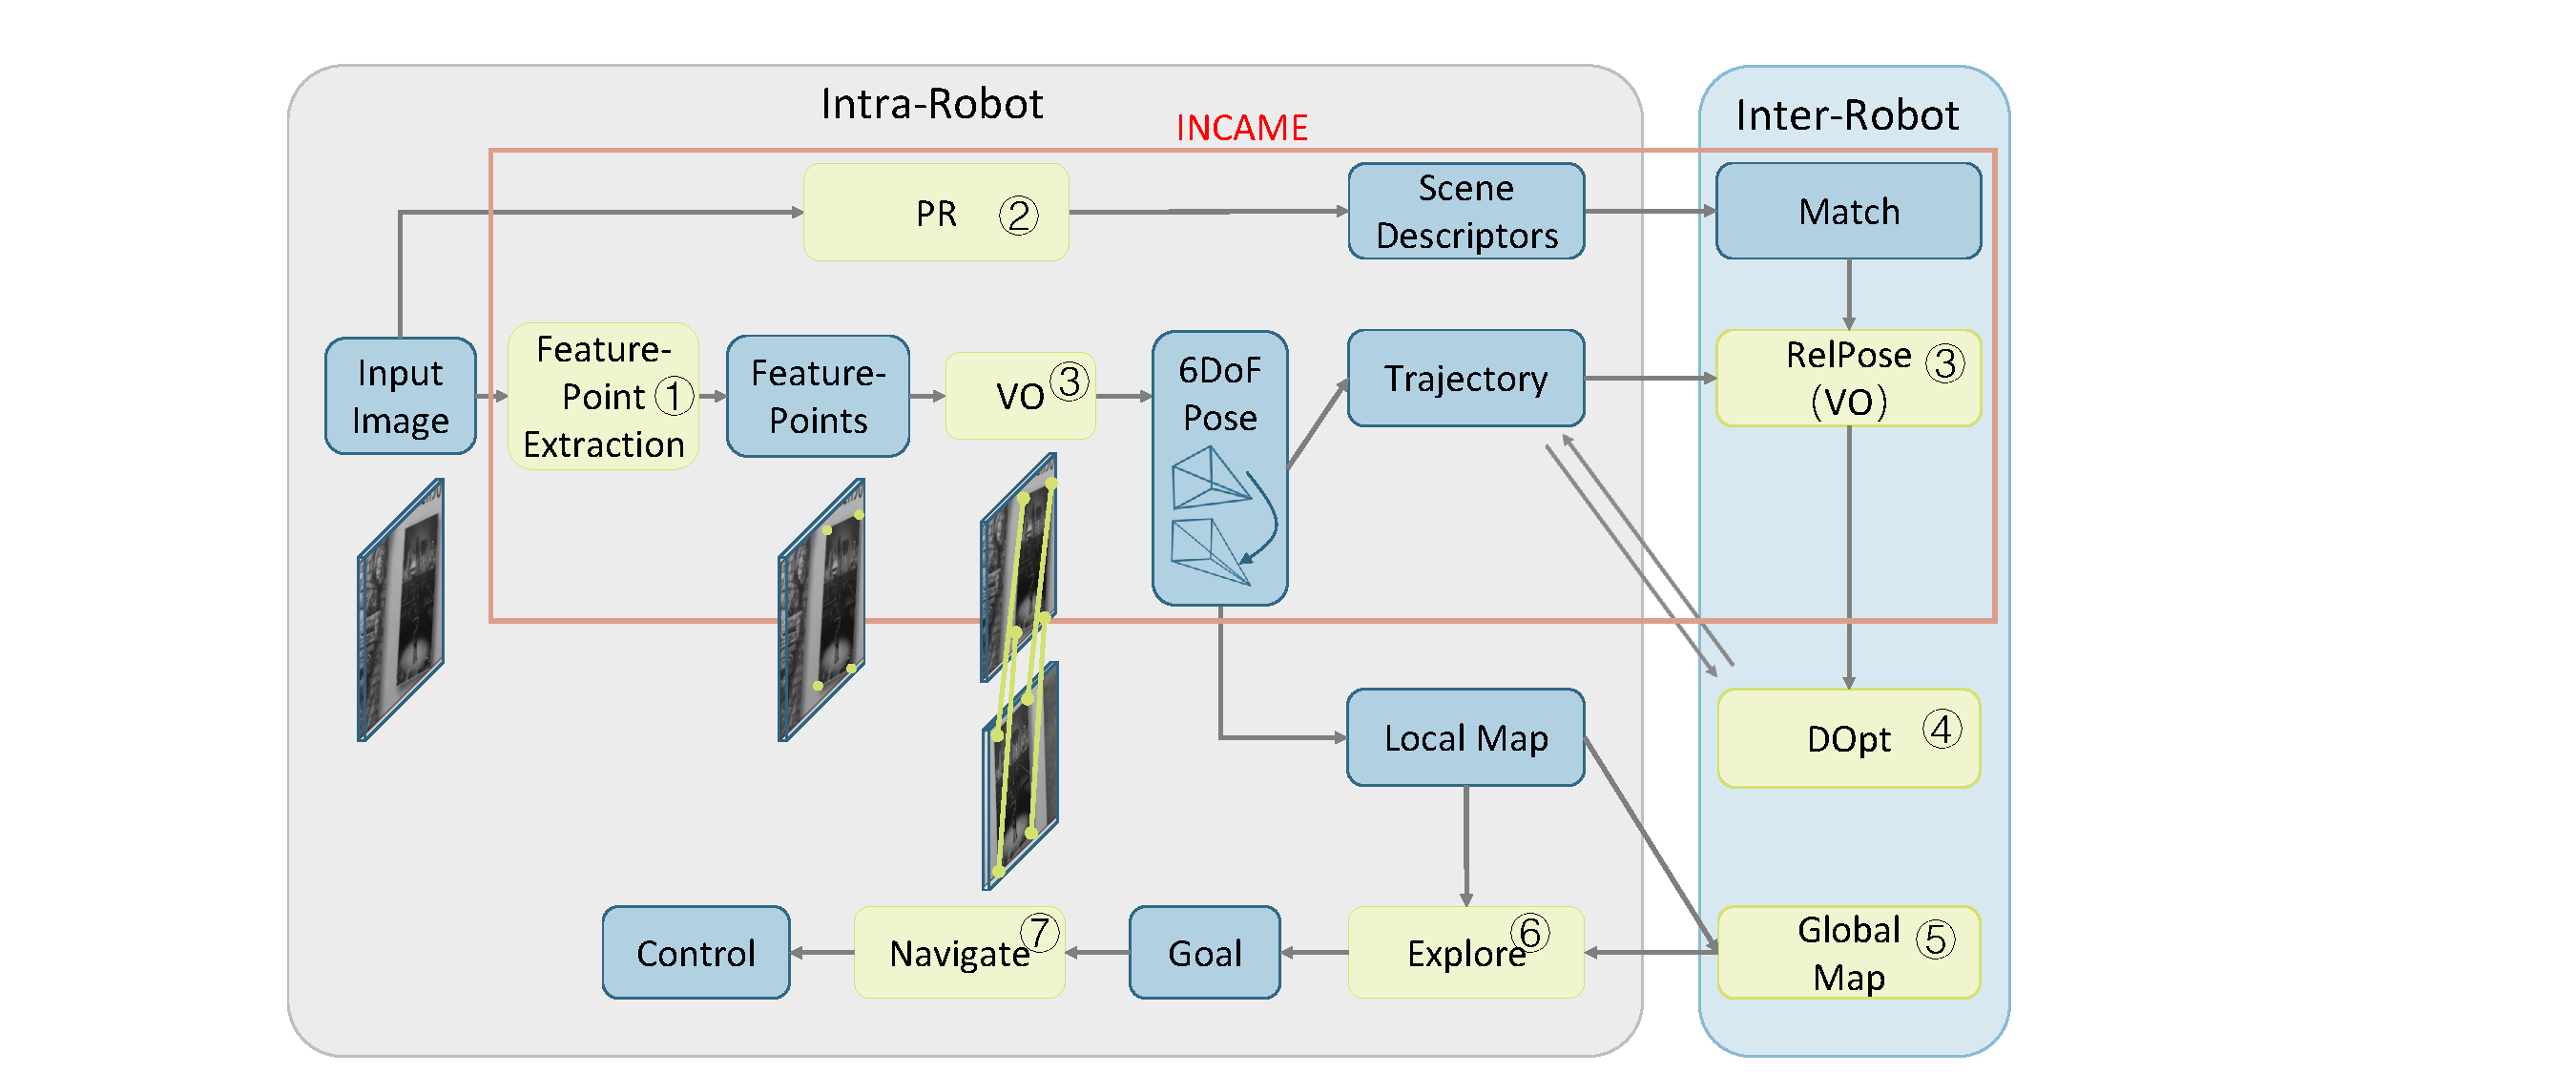
\includegraphics[width=0.99\linewidth]{fig/maexp.pdf}
     \caption{
        The components in MR-Exploration.  Each frame is required to execute \textcircled{1}\textcircled{3} with low latency. \textcircled{2} runs on some key frames. INCAME implements \textcircled{1} \textcircled{2} on the CNN accelerator, and optimizes the scheduling among \textcircled{1} \textcircled{2}  \textcircled{3}.
    }
%     \caption{
%         The components in MR-Exploration. \textcircled{1}\textcircled{3} are basic for a single robot, should be execute every frame. \textcircled{2} generates representation code for some key frames. \textcircled{4}\textcircled{5} are only executed when representation codes are matched across robots and they are latency tolerant.  \textcircled{6}\textcircled{7} are used for decision and navigation, also latency tolerant.
%     }
	\label{fig:maexp}
\end{figure}


% \Cref{fig:maexp} illustrates the computation modules in MR-Exploration.
% Feature-point extraction (\textcircled{1}) and visual odometry (VO, \textcircled{3}) should be performed for each input frame, and should be completed before the next frame. 
% Place Recognition (PR, \textcircled{2}) generates the representation code for some key frames, and sends them to other robots. 
% When the  representation codes from different robots are matched, optimization (\textcircled{7}) and map merging ((\textcircled{8})) are performed to merge the trajectories and maps. \textcircled{4}\textcircled{5}\textcircled{6} are for decision-making and navigation based on the merged maps. 




\begin{figure*}[t]
    % \flushleft
    \centering
    % \vspace{-0.3cm} 
    % \setlength{\abovecaptionskip}{0cm} 
    % \setlength{\belowcaptionskip}{-0.2cm} 
	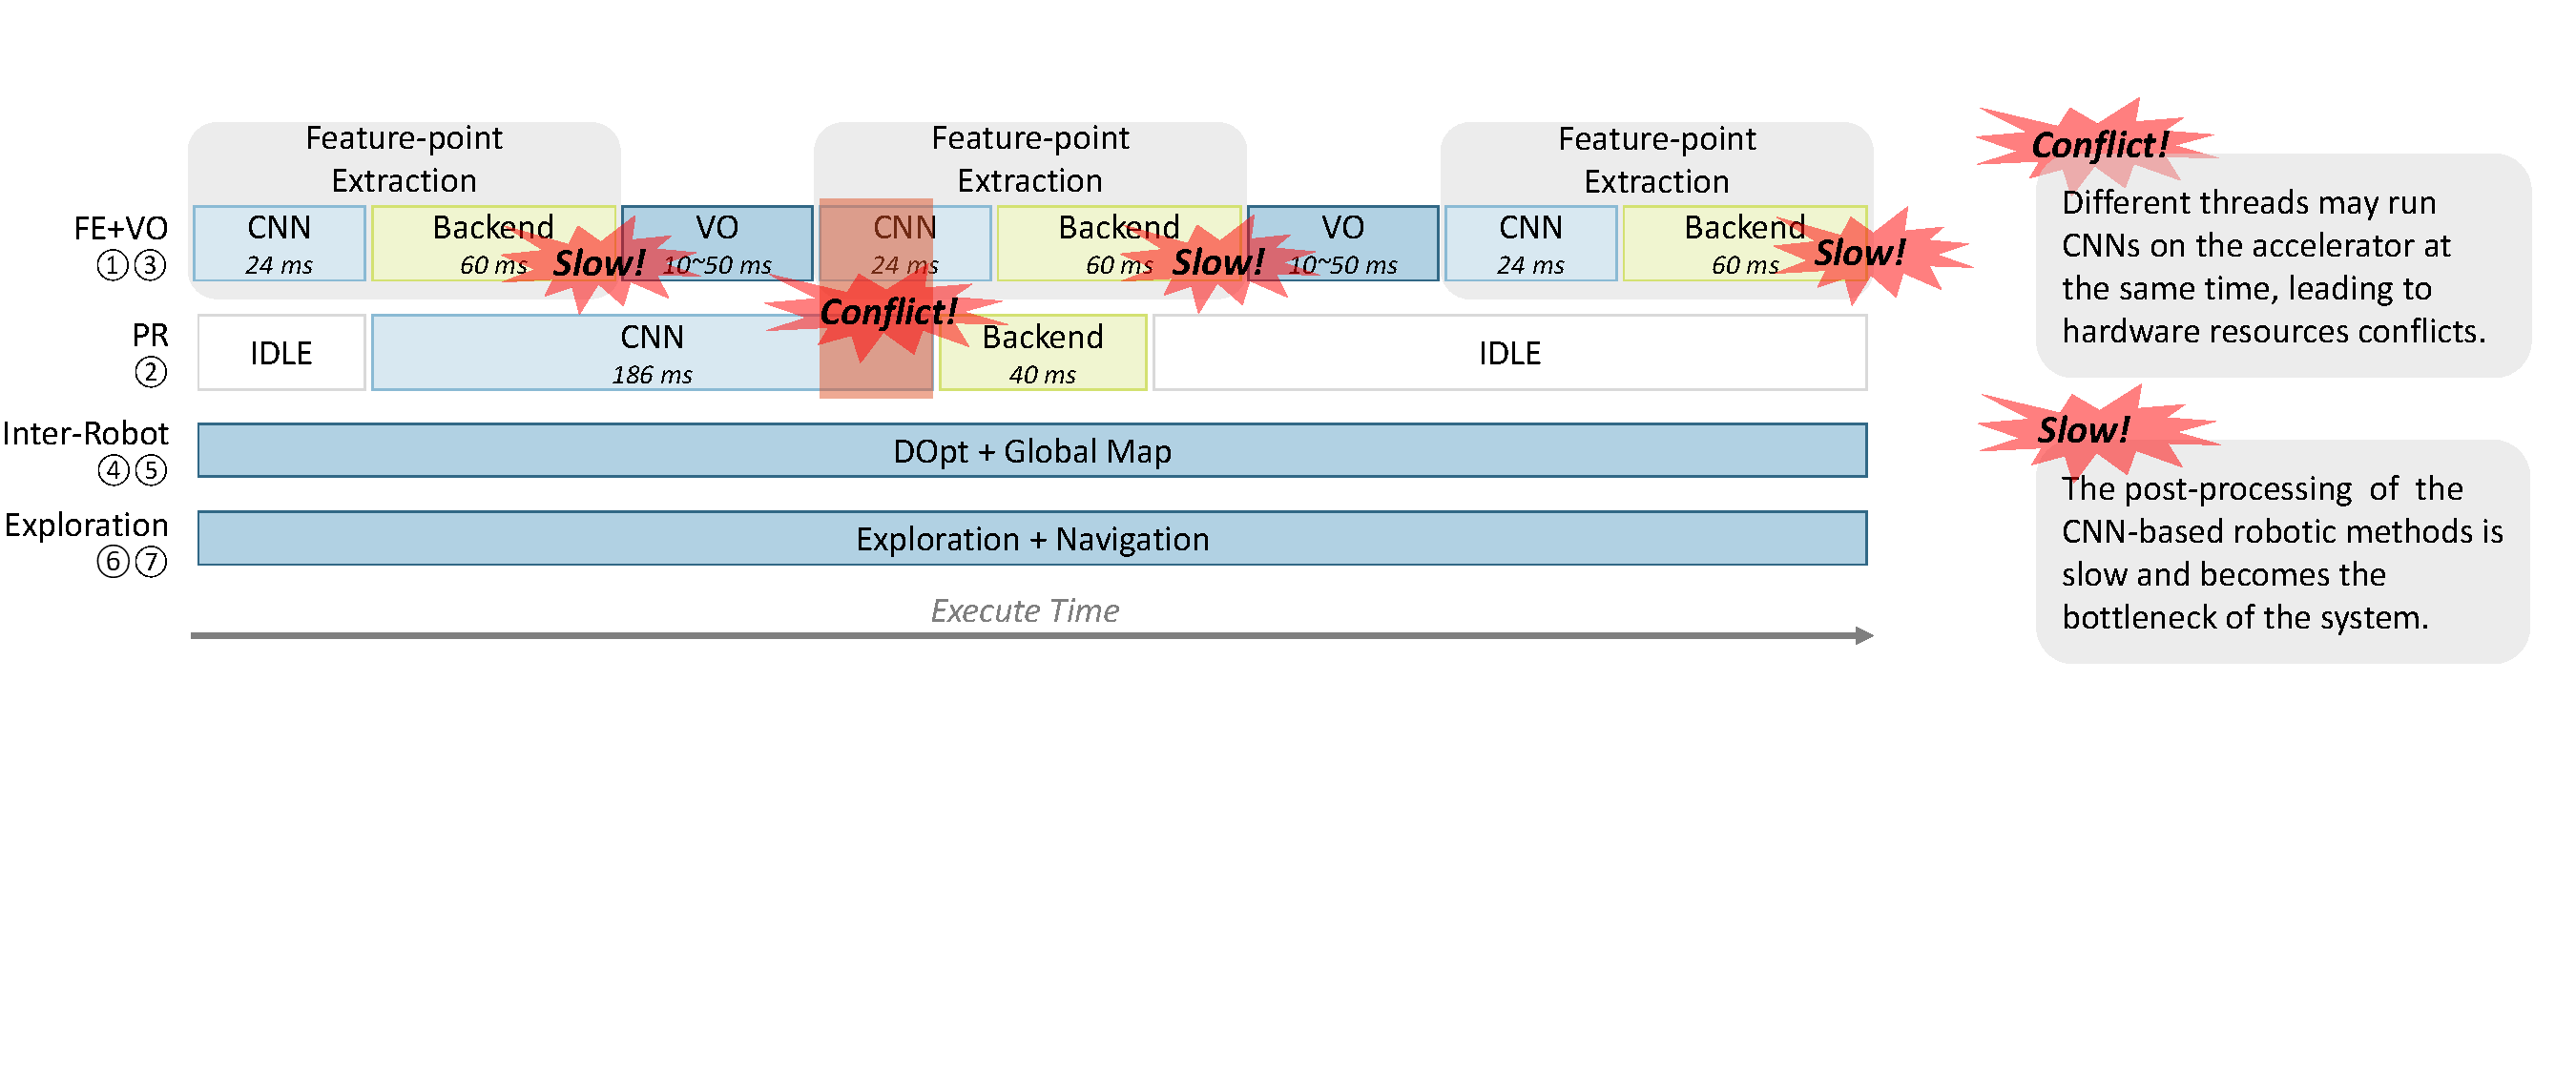
\includegraphics[width=0.99\textwidth]{fig/overalltime.pdf} 	
    \caption{
    The overall timeline of MR-Exploration.
    }
	\label{fig:overalltime}
\end{figure*}

Recent works use CNN to extract feature-points  ~\cite{detone2018superpoint, simo2015discriminative, yi2016lift} and generate the place representation code  ~\cite{arandjelovic2016netvlad, radenovic2018fine}. 
The CNN-based feature-point extraction method, SuperPoint  ~\cite{detone2018superpoint}, achieves 10\%-30\% higher matching accuracy compared with the popular handcrafted extraction method, ORB ~\cite{Mur-Artal:2017281}.
The accuracy of the place recognition code from another CNN-based method, GeM  ~\cite{radenovic2018fine}, is also about 20\% better than the handcrafted method, rootSIFT  ~\cite{jegou2014triang}.

% Thus, we adopt these CNN methods to realize Feature-point Extraction and  Place Recognition. 
Therefore, CNN is increasingly used in robotic systems. 
Besides these two components, more CNN-based methods, such as semantic segmentation  ~\cite{long2015fully} and object detection  ~\cite{ren2015faster}, can be introduced into robots to achieve better performance in the future.

However, CNN is computation consuming. A single inference forward of the CNN-based SuperPoint feature-point extraction consumes 39G operations  ~\cite{detone2018superpoint}, and a single inference forward of the CNN-based GeM  place recognition consumes 192G operations  ~\cite{radenovic2018fine}.
Thus, specific hardware architectures on FPGA  ~\cite{guo2017angel,yu2018instruction,li_high_2016,qiu2016going,lu_evaluating_2017} are designed to deploy CNN on the embedded system.
With the help of network quantization and on-chip data reuse, the speed of CNN accelerators on embedded FPGA achieves 3TOP/s  ~\cite{lu_evaluating_2017}, which can support the real-time execution of CNN-based feature-point extraction  ~\cite{detone2018superpoint}.
However, these CNN accelerators are designed and optimized to accelerate a single CNN. They can not automatically schedule two or more tasks simultaneously. 
% Even if only FE and PR are implemented in CNN, the computational complexity reaches 1 TOP/s , which poses a challenge to the real-time performance of embedded systems.


% In recent years, FPGA is becoming a promising platform for algorithm acceleration. 

We do a simple profiling of MR-Exploration with the CNN accelerator. The CNN backbones of FE and  PR are executed on the FPGA accelerator( Angel-Eye ~\cite{guo2017angel} ).
Other operations, including the post-processing of the CNN-based FE and PR, run on the PS side of Xilinx ZCU102 evaluation board ~\cite{zcu102}. The timeline of each component is illustrated in \Cref{fig:overalltime}. 
The threads of FE and PR may need to process CNN at the same time,  and the simultaneous requests of the accelerator will lead to hardware resources conflicts. The inability of CNN accelerators to support multi-task makes it difficult for researchers in robotics to use embedded FPGA.

In order to facilitate robotic researchers to run different CNN tasks simultaneously on the FPGA accelerator, the accelerator should support the following features:

\textbf{Multi-thread:} Different components in a robot are from different developers. Thus, Robot Operating System (ROS)  ~\cite{quigley2009ros} is proposed as a middleware to fuse these independent components, and is widely used by robotic researchers. Each component is considered as an independent thread in ROS. Different threads should have independent access to the accelerator without knowing the status of others.


% A robot contains many components including perception, decision-making, and control. 
% The Robot Operating System (ROS)  ~\cite{quigley2009ros} is a popular middleware fusing different components from different developers. 
% In ROS, each module is considered as an independent thread on CPU. 
% Different threads should have easy access to the FPGA accelerator.

\textbf{Dynamic Scheduling:} The execution of CNN depends on other operations, like VO module. 
These operations are running on the CPU, and the execution time varies with the input data  ~\cite{mohanan2018survey} (10ms - 50ms for VO, in \Cref{fig:overalltime}). 
The accelerator cannot predict when to start a task. 
Therefore, the FPGA accelerator should be scheduled dynamically to support irregular task requests from the software.

\textbf{Scheduling by priority:} Different components have different priorities. The control and perception tasks usually have higher priorities, while the long-term decision and optimization have lower priorities  ~\cite{RamsauerKLM17}. The critical tasks, which are latency-sensitive,  need to be processed firstly on the accelerator.

The concept of interrupt  ~\cite{jen1974processor} is introduced to CPU in the 1960s. It enables the CPU to support dynamic multi-task scheduling by priority, thus satisfying these three features. Therefore, we introduce the concept of interrupt to the CNN accelerator in this paper to support multi-task on FPGA-based accelerators.

Besides the CNN backbones, the post-processing of the CNN-based methods, including normalization, softmax, rank, etc., are also computation consuming. As illustrated in \Cref{fig:overalltime}, the execution time of post-processing for FE on embedded CPU (~60ms) exceeds that of CNN backbone on the accelerator (30ms), and becomes the bottleneck of the system.

To address the above challenges, we propose an INterruptible CNN Accelerator for Multi-robot Exploration (INCAME) for rapid deployment of robot application on FPGA, with the following contributions:

\begin{itemize}
    % \begin{itemize}[leftmargin = 10 pt]
% \item We propose a CNN-based MR-Exploration framework based on FPGA. The hardware and software modules in INCAME is designed for ROS  ~\cite{quigley2009ros}, so that the modules can be easily used in other applications.
\item We propose a CNN-based MR-Exploration framework, INCAME. CNN-based methods for feature-point extraction (FE) and place recognition (PR) are accelerated with FPGA on ROS platform ~\cite{quigley2009ros}. With the help of the unified interface in ROS, these CNN-based methods can be easily used by other developers in different applications.
\item We propose a \textbf{virtual-instruction-based} interrupt method to make the CNN accelerator support dynamic multi-task scheduling by priority. The method solves the hardware resources conflicts when accelerating different CNN tasks on ROS.
\item We optimize the data flow of the post-processing operations. Hardware modules are also designed for the optimized post-processing. This software-hardware co-optimization assures the MR-Exploration real-time.
\end{itemize}

The rest of this article is organized as follows: \Cref{sec:relate} introduces the related work. \Cref{sec:incame} introduces the INCAME framework with ROS. \Cref{sec:cnninterrupt} details the {virtual-instruction-based} interrupt. \Cref{sec:hardsoftcodesign} details the optimization of post-processing.  Experimental results and analysis are given in \Cref{sec:experiments}. \Cref{sec:conclusion} concludes this article.

\section{RELATED WORK}

\label{sec:relate}


\begin{figure*}[t]
	\centering
    % \vspace{-0.1cm} 
    % \setlength{\abovecaptionskip}{0cm} 
    % \setlength{\belowcaptionskip}{-0.2cm} 
	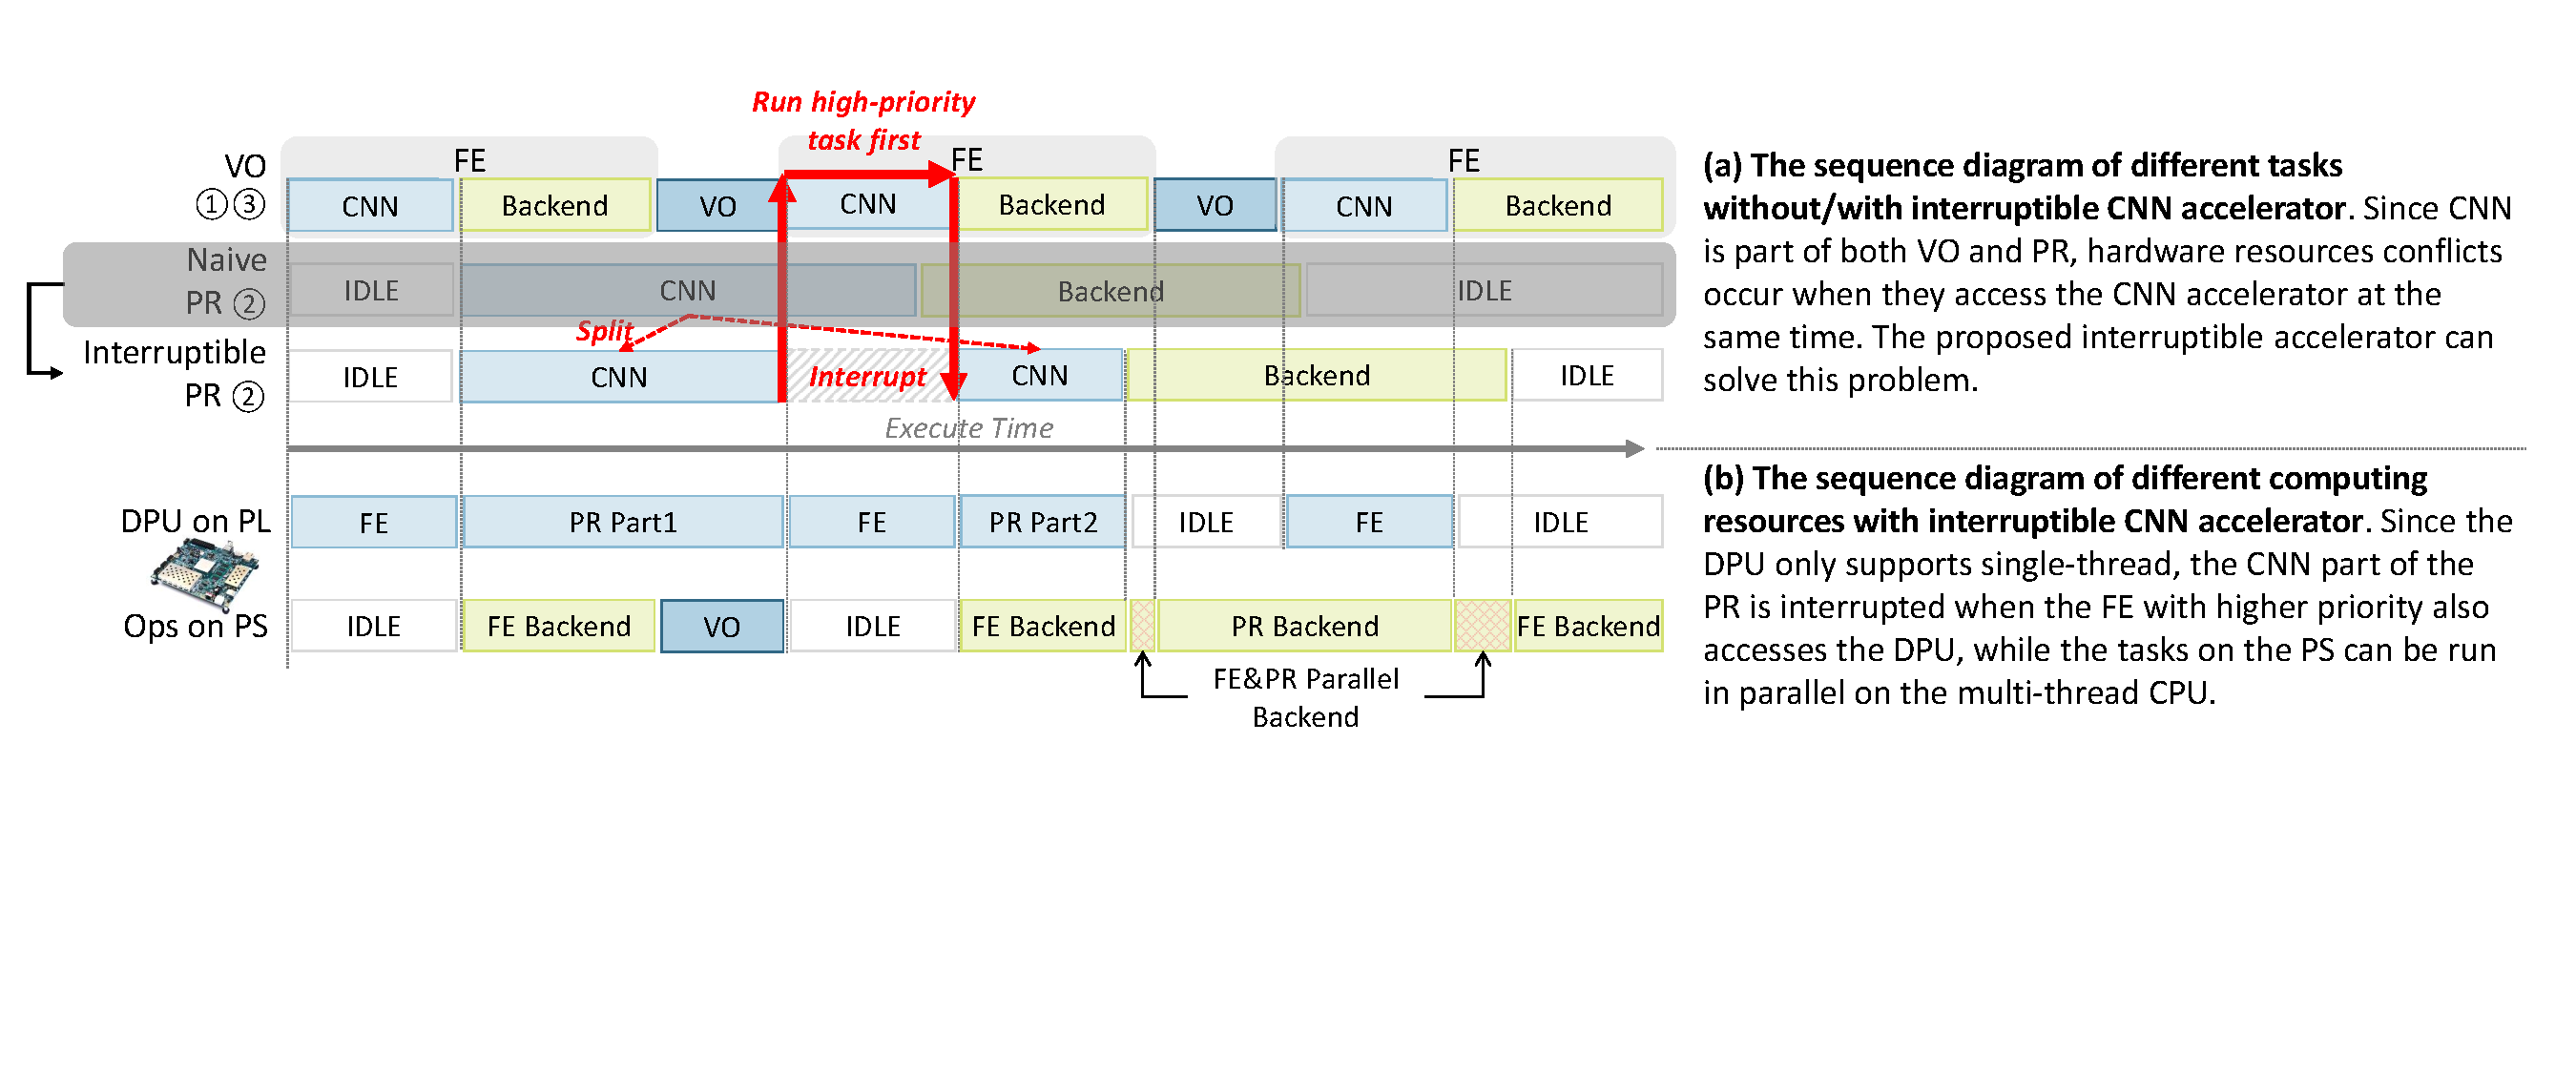
\includegraphics[width=0.95\linewidth]{fig/interDPR.pdf}
    \caption{Interruption to solve the hardware resources conflicts.  
    % When a high-priority task (FE) is started before the low-priority task (PR) is completed, the CNN accelerator backs up the status of PR to memory, and processes the FE task. When the high-priority task is completed, the low-priority task resumes and continues.
    }
	\label{fig:interDPR}
\end{figure*}


\subsection{ CNN-based FE and PR }

\textbf{\quad \ Feature-point extraction:} Previous feature-point extraction works usually consist of two parts: 1) feature-point detection to find the positions of feature-points and 2) descriptor generation to describe the extracted feature-point with a code.
SIFT  ~\cite{Lowe-478}  detects and describes feature-points. The SIFT descriptor is rotation and scale invariant, so that the relative pose transformation between input images via matching SIFT feature-points is accurate. However, the computation of SIFT is complicated and slow  ~\cite{bay2006surf}. Thus, some other handcrafted methods, such as SURF ~\cite{bay2006surf} and ORB  ~\cite{Mur-Artal:2017281}, are proposed as fast alternatives to SIFT. ORB  ~\cite{Mur-Artal:2017281} method is widely used for its balance between speed and accuracy.
Recently, CNN is used to extract feature-points.  ~\cite{simo2015discriminative} proposes a CNN-based descriptor generator that exceeds ORB in accuracy.
SuperPoint  ~\cite{detone2018superpoint} presents a fully CNN-based feature-point extraction method that implements feature-point detection and descriptor generation using one CNN network. SuperPoint ~\cite{detone2018superpoint} reaches 10\%-30\% higher matching accuracy compared with the ORB-based feature-point extraction  ~\cite{Mur-Artal:2017281}. 
% SuperPoint is used in this work.

\textbf{Place recognition:} Before CNN-based place recognition, Bag of Words (BoW)  ~\cite{small_1} relying on handcrafted features is the most popular method. The accuracy of BoW-based methods is strongly influenced by the codebook size ( descriptor length ). Larger codebooks (1MB $\sim$ 10MB)  ~\cite{large_1, large_2} can compete with CNN-based methods in accuracy. However, they take up huge storage and communication resources. Smaller codebooks ~\cite{small_1, small_2, jegou2014triang} require less space but get worse accuracy. In contrast to traditional methods, CNN-based methods not only perform well but also generate more compact features, saving storage and communication resources. GeM  ~\cite{radenovic2018fine} and NetVLAD  ~\cite{arandjelovic2016netvlad} are popular CNN-based methods for their accuracy and data efficiency. GeM  ~\cite{radenovic2018fine} is 20\% better than the handcrafted method rootSIFT  ~\cite{jegou2014triang}.

Due to the advantage of CNN in image-based tasks, more and more CNN-based methods are used in the robotic system.


\subsection{ FPGA accelerators for a specific robot task }

The feature-point extraction (FE) operation is the fundamental component of a vision-based robot, and is also one of the most time-consuming components  ~\cite{fang2017fpga}.
Some previous works design hardware architectures for FE.
SRI-SURF  ~\cite{jia2016sri} optimizes the memory access to speed up SURF  ~\cite{bay2006surf} feature-point extraction. 
~\cite{fang2017fpga} directly implements ORB on FPGA using HLS. eSLAM ~\cite{liu2019eslam} optimizes the ORB algorithm and designs hardware for better performance.
Some other works design architectures for the entire robot system. Hero  ~\cite{shi2018hero} is a framework for navigation and laser-based robot and cannot support vision-based robots that are much more lightweight and cheaper. 
~\cite{li2019879gops} introduces CNN accelerators for the vision-based robot. 
However, the CNN accelerator in this work ~\cite{li2019879gops} is only used for feature-point extraction, and the accelerator is not to support different tasks at the same time. 
Deploying multiple CNNs on the robotic accelerator can expand the functions of robots, without designing hardware for specific functions.



\subsection{ CNN accelerators }

To accelerate CNN on FPGA, some previous works design frameworks to generate a specific hardware architecture for a target CNN, based on  RTL  ~\cite{li_high_2016} or HLS  ~\cite{lu_evaluating_2017}. These works need to reconfigure the FPGA to switch between different CNN models. The reconfiguration consumes seconds  ~\cite{FPGAPerformance}, which is unacceptable for the real-time system.
Some other works design instruction-driven accelerators  ~\cite{yu2018instruction,qiu2016going,guo2017angel,dpu}, making rapid switching possible by providing different instruction sequences. 
However, the CNN tasks on previous instruction-driven CNN accelerators are not interruptible, resulting in the latency-sensitive high-priority task waiting for the low-priority task to finish. 
This inability of CNN accelerators to support multi-task makes it difficult for robotic researchers to use embedded FPGA.

% However, previous instruction-driven CNN accelerators need to schedule the entire CNN, and can not automatically schedule two or more tasks simultaneously. The inability of CNN accelerators to support multi-task makes it difficult for robotic researchers to use embedded FPGA.

\section{INCAME Framework}
\label{sec:incame}

To solve the hardware resources conflicts when the ROS software accesses the CNN accelerator, we propose the INCAME framework in this section.



\begin{figure}[t]
	\centering
    % \vspace{-0.1cm} 
    % \setlength{\abovecaptionskip}{0.cm} 
    % \setlength{\belowcaptionskip}{-0.25cm} 
    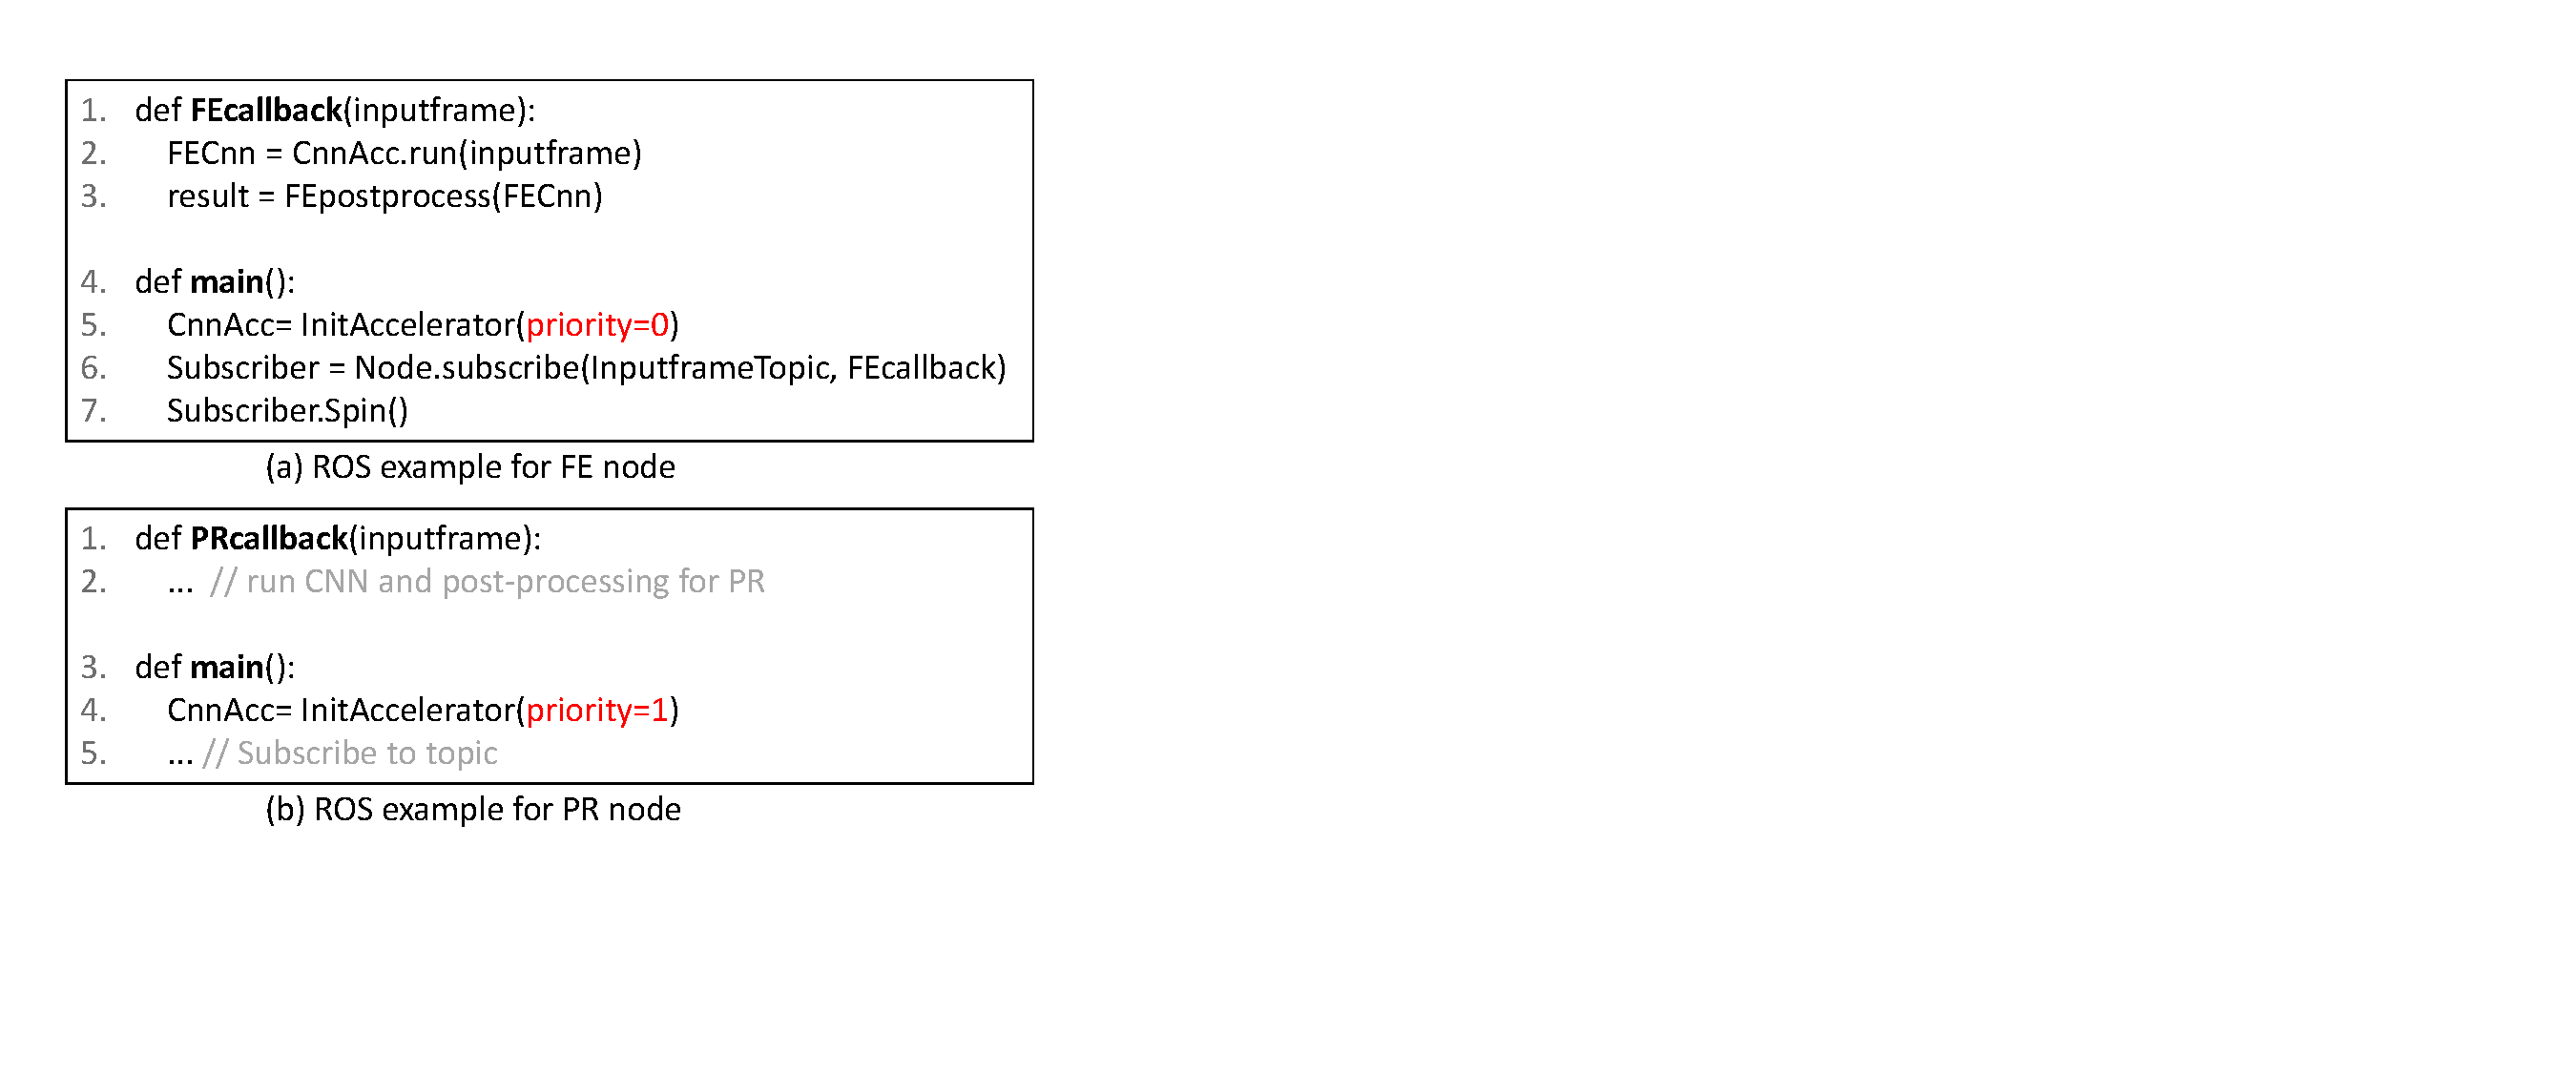
\includegraphics[width=0.9\linewidth]{fig/codeexample.pdf}
    \caption{ ROS code examples.}
	\label{fig:rosexample}
\end{figure}

\begin{figure*}[t]
	\centering
    % \vspace{-0.1cm} 
    % \setlength{\abovecaptionskip}{0cm} 
    % \setlength{\belowcaptionskip}{-0.05cm} 
    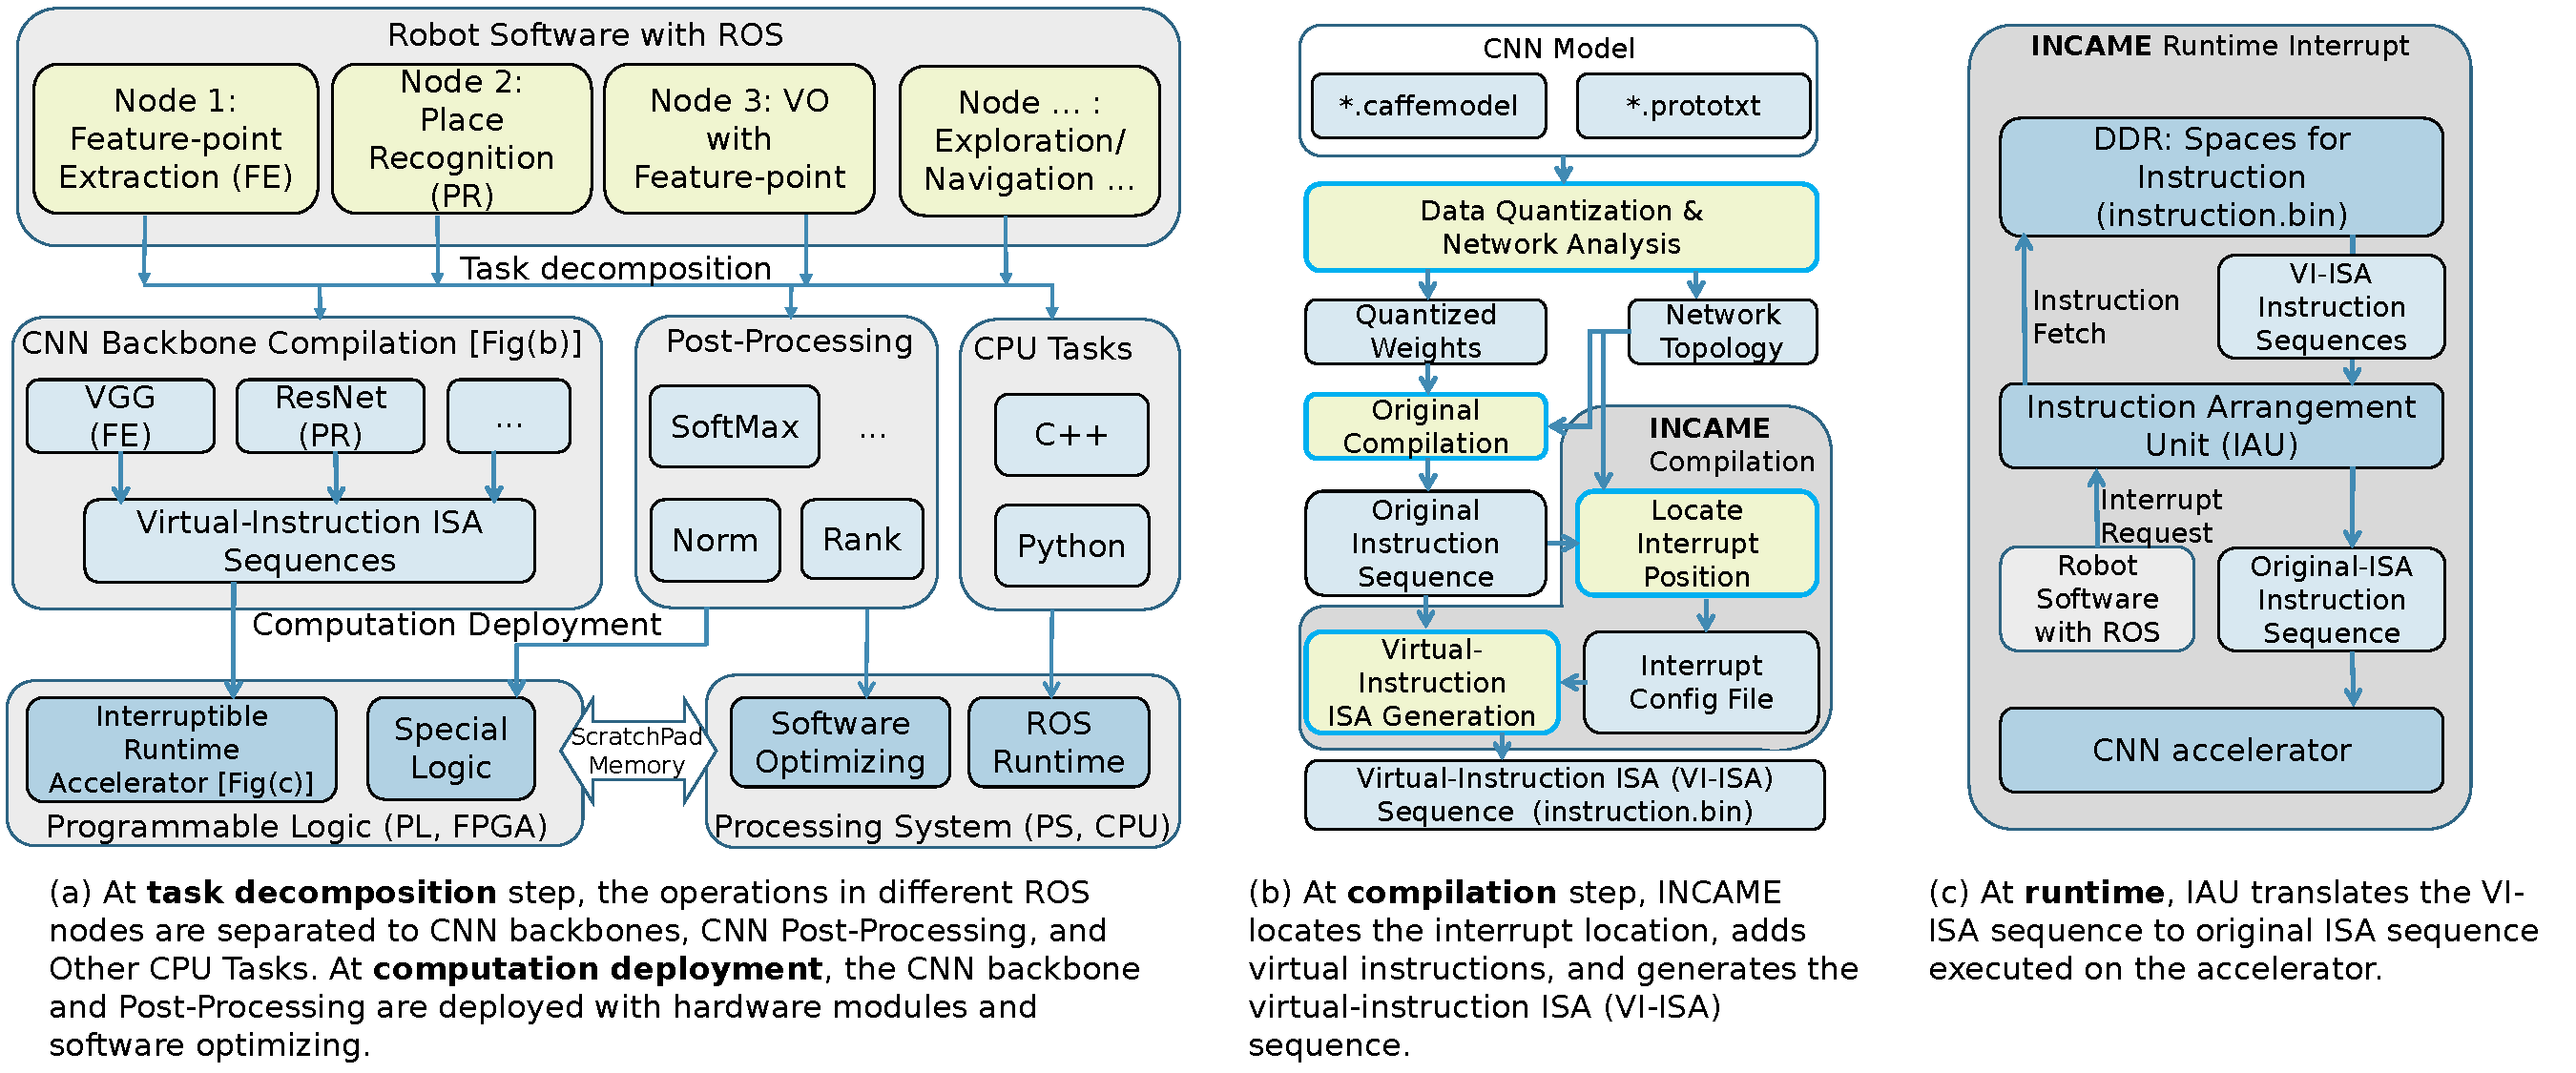
\includegraphics[width=0.99\linewidth]{fig/incame.pdf}
    \caption{ INCAME framework.}
	\label{fig:incame}
\end{figure*}

\subsection{Hardware Resources Conflicts In ROS}
\subsubsection{Introduction to ROS} Building a real robot requires many different components, including sensors, perception algorithms, and control units from different developers. The Robot Operating System (ROS)  ~\cite{quigley2009ros} is proposed to fuse the components from different researchers into a real system.
%  ROS is a popular framework for developing a robot, which provides programming specifications and a communication interface.

Each function module, such as FE, PR, and VO, is called a \textbf{Node} in ROS. Each node is an independent thread running on CPU, and does not know the running status of others. 
% Different nodes communicate with others by \textbf{ROS topics}. 
A node can publish \textbf{ROS topics} and subscribe to topics. The publishing and subscribing nodes connect to the same topic.
% , and neither node needs to know whether the other exists.
The subscribing node processes the received topics with callback functions. Line 6,7 in \Cref{fig:rosexample}(a) bind the topics (InputFrame) with the callback function (FEcallback to extract the feature-points). 


% The publishing node is called publisher, the subscribing node is called subscriber.

% \textbf{Publisher.} When the output of a publisher node is ready, the output data are inmediately packaged to the topic and published. ROS provides some system publisher, such as cv\_camera  ~\cite{cvcamera} to read the camera and publish the input frames to a ROS topic.

% \textbf{Subscriber.} The subscriber processes received topics through \textbf{callback} functions. Each callback function is bound to a topic. When the topic receives data, the callback function executed to process the data. If the callback function cannot complete before receiving the new data, the newly received data will be discarded.


 

% \subsection{Hardware Resources Conflicts in ROS}

\subsubsection{Hardware Resources Conflicts In ROS} Although ROS is becoming the fundamental software platform for robotics, the independence between different ROS nodes brings \textbf{hardware resources conflicts challenge} to access the hardware accelerator. 
% Because developers cannot predict the running state of the CNN accelerator when they write programs, the accelerator may be occupied by other threads when a ROS node needs to call the accelerator. 
\Cref{fig:rosexample}(a) Line 5 and \Cref{fig:rosexample}(b) Line 4 initialize the accelerator for the nodes. Line 2 in \Cref{fig:rosexample}(a) (b) runs the CNN backbone on the accelerator, respectively. Different nodes in ROS initialize and run the CNN accelerator independently, which may result in hardware resources conflicts. To address this problem, we set the priorities of different tasks at the initialization phase (the {\color{red}priority} parameter), and enable the accelerator interrupt to schedule the high-priority task firstly.

% The runtime status of the CNN accelerator is not predictable when developers writing the program. Line 13 in ROSExample1 and line 9 in ROSExample2 initialize the DPU for each task. Line5 in ROSExample1 an d line 3 in ROSExample2 run the tasks on the same CNN accelerator, which may result in hardware conflicts. In INCAME, the priorities of different tasks are configured at initialization phase to address the hardware conflicts problem.


% \begin{algorithm}[t]
%     \caption{ ROS Node for FE }
%     \label{code:FE}
%     \begin{algorithmic}[1]
%         \State {\color{gray} // imagePtr, imageAddr, fmPtr, fmAddr, DPUtask, Bankendtask  is initialized by main and used in FEcallback.}
%         \Function {FEcallback}{$ InputFrame $}
%         \State {\color{gray} // Read and reshape the InputFrame. }
%         \State {\color{blue} *imagePtr  $\gets$ *InputFrame }
%         \State DPUtask.run()
%         \State FEBackend.run()
%         \EndFunction

%         \Function {Main}{$ $}
%         \State {\color{gray} // Init ScratchPad Memory. Ptr is for CPU operations, Addr is for FPGA modules.}
%         \State imagePtr, imageAddr = ScratchPad(FEinputsize)
%         \State fmPtr, fmAddr = ScratchPad(FEfmsize)
%         \State {\color{gray}// Config task0 in IAU of the accelerator (DPU).}
%         \State DPUtask = DPUinit({\color{red}  priority=0},{\color{blue} instraddr=FEinstrAddr, }
%         \State \qquad \qquad \qquad \quad {\color{blue} inoffset=imageAddr,outoffset=fmAddr } ) 
%         \State FEBackend = FEBackendinit({\color{blue}fmAddr, fmPtr});
%         \State {\color{gray}// The node subscribes the inputframe, and use the FEcallback to process each inputframe.}
%         \State Subscriber = Node.subscribe( InputFrameTopic, FEcallback);
%         \State {\color{gray}// Use spin to start the subscriber}
%         \State Subscriber.spin();
%         \EndFunction
%     \end{algorithmic}
% \end{algorithm}

% \begin{algorithm}[t]
%     \caption{ ROS Node for PR }
%     \label{code:PR}
%     \begin{algorithmic}[1]
%         \Function {PRcallback}{$ InputKeyFrame $}
%         \State {\color{blue} *imagePtr  $\gets$ *InputKeyFrame }
%         \State DPUtask.run()
%         \State PRBackend.run()
%         \EndFunction

%         \Function {Main}{$ $}
%         \State imagePtr, imageAddr = ScratchPad(PRinputsize)
%         \State fmPtr, fmAddr = ScratchPad(PRfmsize)
%         \State DPUtask = PR\_DPUinit( {\color{red} priority=1},{\color{blue} instraddr=PRinstrAddr}, 
%         \State \qquad \qquad \qquad \quad {\color{blue} inoffset=imageAddr,outoffset=fmAddr } ) 
%         \State PRBackend = PRBackendinit({\color{blue}fmAddr, fmPtr});
%         \State Subscriber = Node.subscribe( InputKeyFrameTopic, PRcallback);
%         \State Subscriber.spin();
%         \EndFunction
%     \end{algorithmic}
% \end{algorithm}

% \subsection{ Accelerator interrupt to solve Hardware Resources Conflicts }

% In order to support multi-task scheduling and solve the hardware resources conflicts, interrupt is introduced to CPU  ~\cite{jen1974processor}. In this paper, we also use the concept of interrupt to support multi-task on the CNN accelerator.


% If the CNN accelerator supports interrupt, it can run two or more CNN modules at the same time. 
\subsubsection{Accelerator interrupt} \Cref{fig:interDPR} illustrates the idea of interrupt to schedule two CNN tasks. In the process of running a low-priority network (PR), the software may send an execution request for the high-priority task (FE). The interrupt enables the CNN accelerator to backup the running state of the low-priority PR network. Then the accelerator switches to the high-priority FE network. After the high-priority task (FE) completes, the low-priority task (PR) is restored to the accelerator and continues to execute.
% With the help of accelerator interrupt, the execution of the low-priority task (PR) is divided into pieces, and each piece is allocated to the time interval of running different high-priority networks (FE). 
% Accelerator interrupt multiplexes the time division of the accelerator, reduces the idle time of the accelerator, and improves the utilization of hardware resources. 





\subsection{ Interruptible Accelerator with ROS (INCAME) }

% We try to use CNN as much as possible to accomplish various tasks on the robot. Because the CNN not only has advantages over traditional algorithms in accuracy, but also has uniform and regular computing mode. Therefore, a single instruction-driven CNN accelerator can speed up different tasks. The unified accelerator can reduce the use of hardware resources and make it easier to implement the robot computing system on embedded FPGA.

\Cref{fig:incame}(a) illustrates the proposed two-step INCAME framework for mapping ROS based software to embedded FPGA.
The first step is the task decomposition, which decomposes the computation in ROS nodes into different INCAME computation types, including CNN backbones, CNN post-processing, and other CPU tasks. 

The second step is to deploy the computation onto the FPGA. 
The CNN backbones of different tasks, such as the VGG model  ~\cite{kim2016accurate} in SupoerPoint feature-point extraction  ~\cite{detone2018superpoint} and the ResNet101 model  ~\cite{he2016deep} in GeM place recognition  ~\cite{radenovic2018fine}, are compiled to the interruptible Virtual-Instruction Instruction Set Architecture (VI-ISA), which runs on the CNN accelerator. The VI-ISA is a simple extension of the original ISA, in which the extension method is not limited to a specific original ISA. Thus, the virtual-instruction-based interrupt can be easily applied to various instruction-based CNN accelerators  ~\cite{yu2018instruction,qiu2016going}, such as Angel-Eye ~\cite{guo2017angel} and DPU ~\cite{dpu}.
% At runtime, the interruptible CNN accelerator runs these instructions to calculate the CNN backbones.
% To accelerate the post-processing operations of the CNN based methods, 

Hardware modules are implemented for the CPU-intensive Softmax  ~\cite{Softmax-wiki} and Normalization  ~\cite{Norm}. Some task-related software optimizations, such as Ranking and Non-Maximum Suppression (NMS)  ~\cite{NeubeckGool-NMS}, as well as other ROS tasks written in C++/Python, are processed on the CPU side.

To eliminate the memory copy between CPU cores and CNN accelerators, we use low-latency ScratchPad memory  ~\cite{Banakar2002Scratchpad} to directly feed the results from CNN backbones to the post-processing modules. 

\Cref{fig:incame}(b) details the INCAME compilation step and runtime interrupt. Caffe  ~\cite{jia2014caffe} is a popular software framework for CNN, and the *.caffemodel/*.prototxt files define the network parameters and structure in Caffe. The previous deployment process, such as Angel-Eye  ~\cite{guo2017angel} and DPU ~\cite{dpu}, quantizes the weights, and analyze the network topology. The original compiler translates the network topology and the quantization information into the original ISA sequence. INCAME goes further than previous CNN compilers. It selects the optimized interrupt positions in the original instruction sequence, and adds virtual instructions at these positions to enable accelerator interrupt. After that, the original instruction sequence and the added virtual instructions are wrapped to the new interruptible VI-ISA. The wrapped VI-ISA instructions are dumped into a file (instruction.bin), and can be loaded into the instruction spaces on FPGA's DDR.


As illustrated in \Cref{fig:incame}(c), at runtime, an Instruction Arrangement Unit (IAU) in hardware listens to the interrupt request from ROS software, fetches the corresponding VI-ISA interruptible instructions and translates them to the original ISA executed on the CNN accelerator in Angel-Eye  ~\cite{guo2017angel}. 
The detail of the Virtual-Instruction ISA (VI-ISA) and instruction arrangement unit (IAU) is introduced in \Cref{sec:cnninterrupt}. Although INCAME can be applied to various instruction-based CNN accelerators, we implement and evaluate it based on Angel-Eye  ~\cite{guo2017angel}.



\section{Virtual-instruction-based Accelerator Interrupt}
\label{sec:cnninterrupt}
% The idea of interruption is introduced for dynamic multi-task scheduling. This section details the implementation of our \textbf{Virtual instruction Interruption}. \Cref{fig:interDPR} illustrates the idea of interruption to full utilize the hardware resources.


% \begin{figure*}[t]
% 	\centering
% 	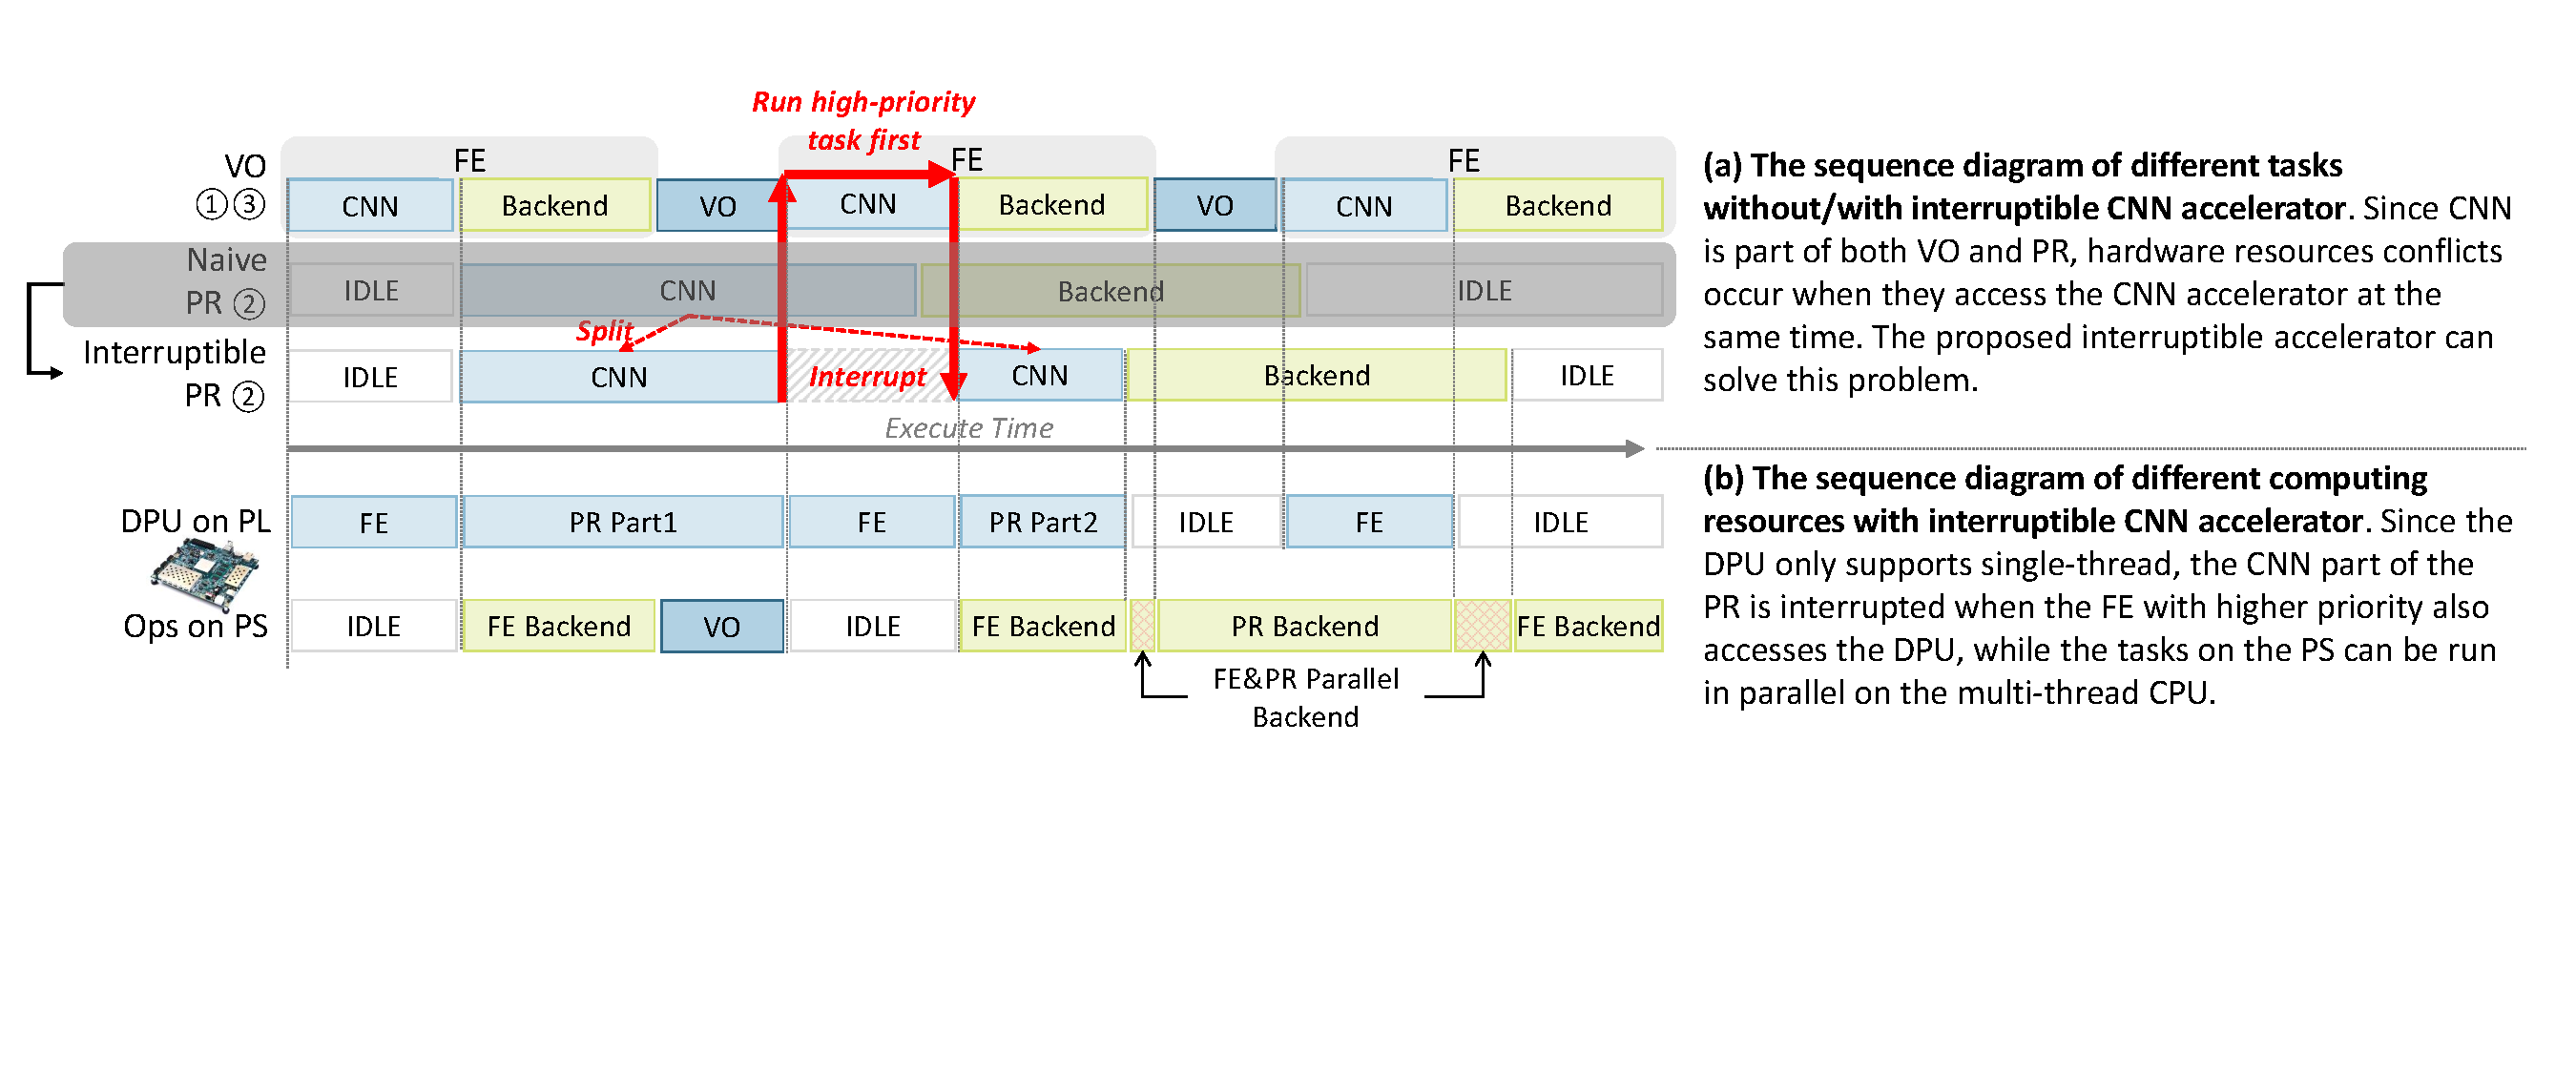
\includegraphics[width=0.99\linewidth]{fig/interDPR.eps}
% 	\caption{Interruption to solve the hardware resources conflicts.  When a high-priority task (FE) is started before the low-priority task (PR) is completed, the CNN accelerator backs up the status of PR to memory, and processes the FE task. When the high-priority task is completed, the low-priority task resumes and continues.
%     }
% 	\label{fig:interDPR}
% \end{figure*}


\begin{table*}[t]
	\footnotesize
	\centering
	\caption{Description for the basic instructions.}
% Table generated by Excel2LaTeX from sheet 'Sheet3'
%\linespread{1.1}\selectfont
\begin{tabular}{|m{2.7em}<{\centering}|m{3.4em}<{\centering}|m{17em}|m{4.2em}<{\centering}|m{4.6em}<{\centering}|m{4.2em}<{\centering}|m{4.2em}<{\centering}||m{6.5em}<{\centering}|m{6.5em}<{\centering}|}
	\hline
	\multicolumn{1}{|c|}{Category} & \multicolumn{1}{c|}{Type} & \multicolumn{1}{c|}{Description} & \multicolumn{1}{c|}{Address 1} & \multicolumn{1}{c|}{Address 2} & \multicolumn{1}{c|}{Address 3} & \multicolumn{1}{c||}{Workload} & \multicolumn{1}{c|}{Backup} & \multicolumn{1}{c|}{Recovery} \\
	\hline
	\multirow{2}[4]{*}{LOAD} & LOAD\_W & Load weights/bias from DDR to on chip weight buffer. & Off-chip Addr & Weights-buffer Addr & -     & Data  Length & -     & Weight / Inputdata \\
	\cline{2-9}\multicolumn{1}{|c|}{} & LOAD\_D & Load input data from DDR to on-chip data buffer. & Off-chip Addr & Data-buffer Addr & -     & Data  Length & -     & Weight / Inputdata \\
	\hline
	\multirow{2}[4]{*}{CALC} & CALC\_I & Calculate intermediate results (from partial input channels) for some output channels from partial  input channels. & Input  Data Addr & Intermediate Data Addr & Weight Addr & Calc Size & Previous final results / Intermediate data  & Weight / Inputdata /  Intermediate data \\
	\cline{2-9}\multicolumn{1}{|c|}{} & CALC\_F & Calculate the results for some output channels from all input channels. The pooling, bias-adding and element-wise operations are operated in this instructions. & Input  Data Addr & Output  Data Addr & Weight Addr & Calc Size & Finial results & Inputdata \\
	\hline
	SAVE  & SAVE  & Save the results from on-chip data buffer to DDR. & Off-chip Addr & Data-buffer Addr & -     & Data  Length & -     & Inputdata \\
	\hline
	\end{tabular}%
	
	\label{tab:instr}%
  \end{table*}%


\begin{figure}[t]
	\centering
    % \vspace{-0.1cm} 
    \setlength{\abovecaptionskip}{0cm} 
    % \setlength{\belowcaptionskip}{-0.6cm} 
	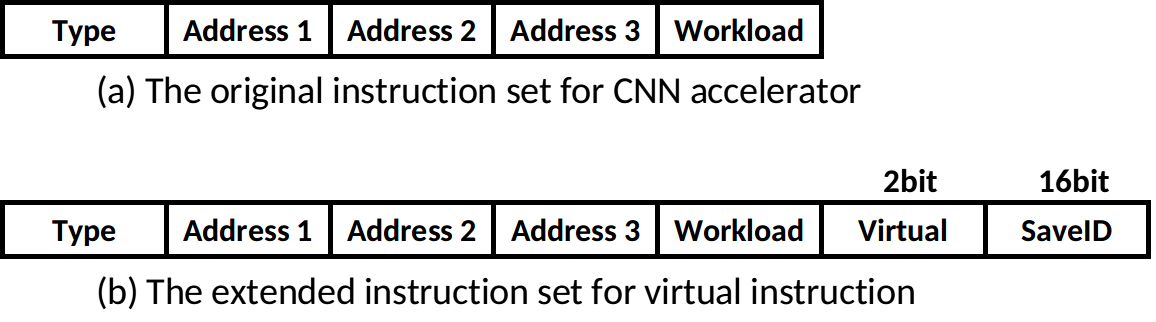
\includegraphics[width=0.99\linewidth]{fig/instructions.png}
	\caption{Original and Virtual-Instruction ISA.}
	\label{fig:instructions}
\end{figure}

In this section, we introduce our \textbf{virtual-instruction-based} method to enable accelerator interrupt. Compared with the CPU-Like and Layer-by-Layer interrupt method, virtual-instruction-based method minimizes the interrupt response latency and the extra cost of interrupt.
% In this section, we introduce our virtual-instruction-based method to enable accelerator interrupt. To minimize the interrupt response latency and extra cost for interrupt, we propose the virtual-instruction-based accelerator interrupt method.

\subsection{ Instruction Driven Accelerator }
\label{sec:instrAcc}
There are three categories of instruction in the instruction-driven accelerator: LOAD, CALC, and SAVE  ~\cite{guo2017angel,qiu2016going,yu2018instruction}. The instruction description of each kind of instruction is listed in \Cref{fig:instructions}(a) and \Cref{tab:instr}.

The LOAD instruction moves input feature-maps and weights from DDR to on-chip memory. The SAVE instruction moves the calculated output features from on-chip memory to DDR. 

Each CALC  instruction,  including CALC\_I and CALC\_F, processes the convolution according to the hardware parallelism with $Para_{height}$ lines from $ Para_{in} $ input channels to $ Para_{out}$ output channels. $Para_{height}$, $ Para_{in} $, and $ Para_{out} $ are the parallelism along the height, input channel and output channel dimensions, which is determined by the hardware and original ISA.

\Cref{fig:singlesave}(a) illustrates the operation of CALC instructions. The convolution of the last $ Para_{in} $ input channels is CALC\_F, and the convolutions for the former input channels are CALC\_I. The CALC\_F and the CALC\_I instructions for the same output channels, as well as the LOAD instructions for corresponding input feature-maps and weights, are considered as a \textbf{CalcBlob}  (\Cref{sec:exampleVirtual}(c) lists an example for CalcBlob). In each CalcBlob, there is a LOAD\_W instruction for the corresponding weights. However, as the input data can be shared across different CalcBlobs, some CalcBlobs do not have  LOAD\_D instruction. 

% Each CALC  instruction,  including CALC\_I and CALC\_F processes the convolution according to the hardware parallelism.
% Each CALC instruction, including CALC\_I and CALC\_F processes the convolution from input feature of the hardware input parallelism ($Para_{in}$) to the output feature of the hardware output parallelism ($ Para_{out}$), as illustrated in \Cref{fig:singlesave}(a). The convolution of the last input channels is CALC\_F, and the convolutions for the former input channels are CALC\_I. The CALC\_F and the CALC\_I instructions to generate the output channels, as well as the LOAD instructions for corresponding input feature-maps and weights are considered as a \textbf{CalcBlob}. Besides the convolution, some other operations like pooling is also represented in the CALC\_F instruction.

% Considerring to the limited on-chip data memory, the on-chip data buffer may not able to store all of the input and output feature-maps. To solve this problem, a CALC instruction is not designed for the entile feature-map, yet servel lines of the feature-map. The parallelism along the height dimension of a CALC instruction is denoted as  





% \subsection{Accelerator Interrupt }

\subsection{How To Interrupt: Virtual Instruction}
\label{sec:howinter}

There are four stages to handle interrupt. For the instruction flow illustrated in \Cref{fig:singlesave}(c), the interrupt stages are shown in \Cref{fig:singlesave}(e), including: (1) Time for finishing the current operation, $t1$. (2) Time to backup, $t2$. (3) Time for the high-priority task, $t3$. (4) Time to restore the low-priority task ,$t4$. The the latency to respond the interrupt is $t_{latency} = t_1+t_2$. The extra cost for interrupt is $t_{cost}=t_2+t_4$. 
There are different methods to implement interrupt in CNN accelerators.

\textbf{CPU-Like.}
When an interrupt request occurs in CPU, CPU backs up all the on-chip registers to DDR. However, there are only tens of registers in CPU, and the volume of the backed-up data is less than 1 KB  ~\cite{furber2000arm}. In CNN accelerators, there are hundreds of KB $\sim$ several MB on-chip caches  ~\cite{qiu2016going, guo2017angel} to store input feature-maps or weights. 
% If all on-chip caches are backed-up/recovered, the cost of data transfer in the accelerator is much higher than that of CPU. 
Thus, the extra data transfer increases both the interrupt response latency($t_{latency}$) and the additional cost ($t_{cost}$).

\textbf{Layer-by-layer.}
Most accelerators run the CNN layer by layer  ~\cite{qiu2016going,guo2017angel}. 
There is no extra data transfer for the accelerator to switch between different tasks after each layer, thus, $t_{cost}=0$. 
However, the position of the interrupt request is irregular and unpredictable. When an interrupt occurs inside a CNN layer, the CNN accelerator needs to finish the whole layer before switching, which leads to the high response latency($t_{latency}$).

% The latency to respond the interrupt and the performance degradation of the CPU-like interrupt and Layer-by-layer method will be evaluated in \Cref{sec:experiments}.



We propose the \textbf{virtual-instruction-based} method to enable low-latency interrupt. 
% Different from the CPU-like interrupt, which backup/recovery all the on-chip caches, only the on-chip cache which is still needed in future execution will be backed-up and restored. So that the amount of data transfer is much lower than that of CPU-like interrupt.
To reduce the interrupt response latency, our virtual-instruction-based method is interruptible inside each layer. We add some virtual instructions to the original instruction sequence to enable the interrupt.
The virtual instructions, which contain the backup and recovery instructions, are responsible for backing up and restoring on-chip caches. 

\textbf{Virtual SAVE} instructions back up the intermediate results from partial input channels or the final output results. There is no need to back up the input feature-maps and weights, because these inputs are already stored in DDR. 

\textbf{Virtual LOAD} instructions restore the input feature-maps from DDR to on-chip caches, because input featuremaps are loaded by one CalcBlob, and shared across subsequent CalcBlobs.
% , and thus the subsequent CalcBlobs do not read the input feature-maps. 
Virtual LOAD instructions also need to restore the intermediate results from partial input channels backed up by the virtual SAVE instructions.

% By adding the virtual instructions, the CNN can be interrupted anywhere, and the latency to respond interrupt is reduced.


% For backup virtual instructions, the corresponding input data and weights are already stored in DDR. 
% Thus, there is no need to back up the input buffer and weight buffer. Only the intermediate data and the final output results are needed to be backed-up. 

% For recovery virtual instructions, the weights and input data, as well as the backed-up intermediate data, are needed to be restored from DDR to the on-chip cache.
% The accelerator can switch to a different task after the backup virtual instructions, and resume the execution by the recovery virtual instructions.

% By adding the virtual instructions, the CNN can be interrupted anywhere, and the latency to to response the interrupt is reduced. However, there virtual instructions are only valid when interrupt occurs. So we add a field in the origin instruction set, that indicates whether the instruction a virtual instruction. If no interrupt occurs, virtual instructions will be skipped and discarded, which can ensure the efficiency of uninterrupted execution. The modifications to the instruction set will be introduced in \Cref{sec:virtualinstr}. 


% However, the CPU-like interrupt would back up all the on-chip registers to DDR. In CPU, there are tens of registers, and the backed-up data is around 1 KB. In CNN accelerators, there are hundreds of KB ~ several MB on-chip cache  ~\cite{qiu2016going, yu2018instruction}. If all the on-chip cache is backed-up and recovered, the cost of data transfer in the CNN accelerator is much higher than that of CPU.

% We propose the \textbf{virtual-instruction-based} method to enable low-latency interrupt. The low-priority task maintains the executing status itself, rather than the hardware or the interrupt handler used in CPU. Only the cache which is still needed in future execution will be backed-up and restored.

% The virtual instructions, which contain the backup and recovery instructions, are generated in the compilation phase, together with the normal instructions. 
% For backup instructions, the corresponding input data and weights are still stored in DDR. 
% There is no need to back up the input buffer and weight buffer, and only the intermediate data and the final output results are needed to be backed-up. 
% For recovery instructions, the weights and input data for future calculation, as well as the backed-up intermediate data, are needed to be restored from DDR to the on-chip cache.

% There is a field in the instruction set, that indicates whether the instruction a virtual instruction. If no interrupt occurs, virtual instructions will be skipped and discarded, which can ensure the efficiency of uninterrupted execution.







\begin{figure*}[t]
    % \flushleft
    \centering
    % \vspace{-0.1cm} 
    \setlength{\abovecaptionskip}{0cm} 
    % \setlength{\belowcaptionskip}{-0.05cm} 
	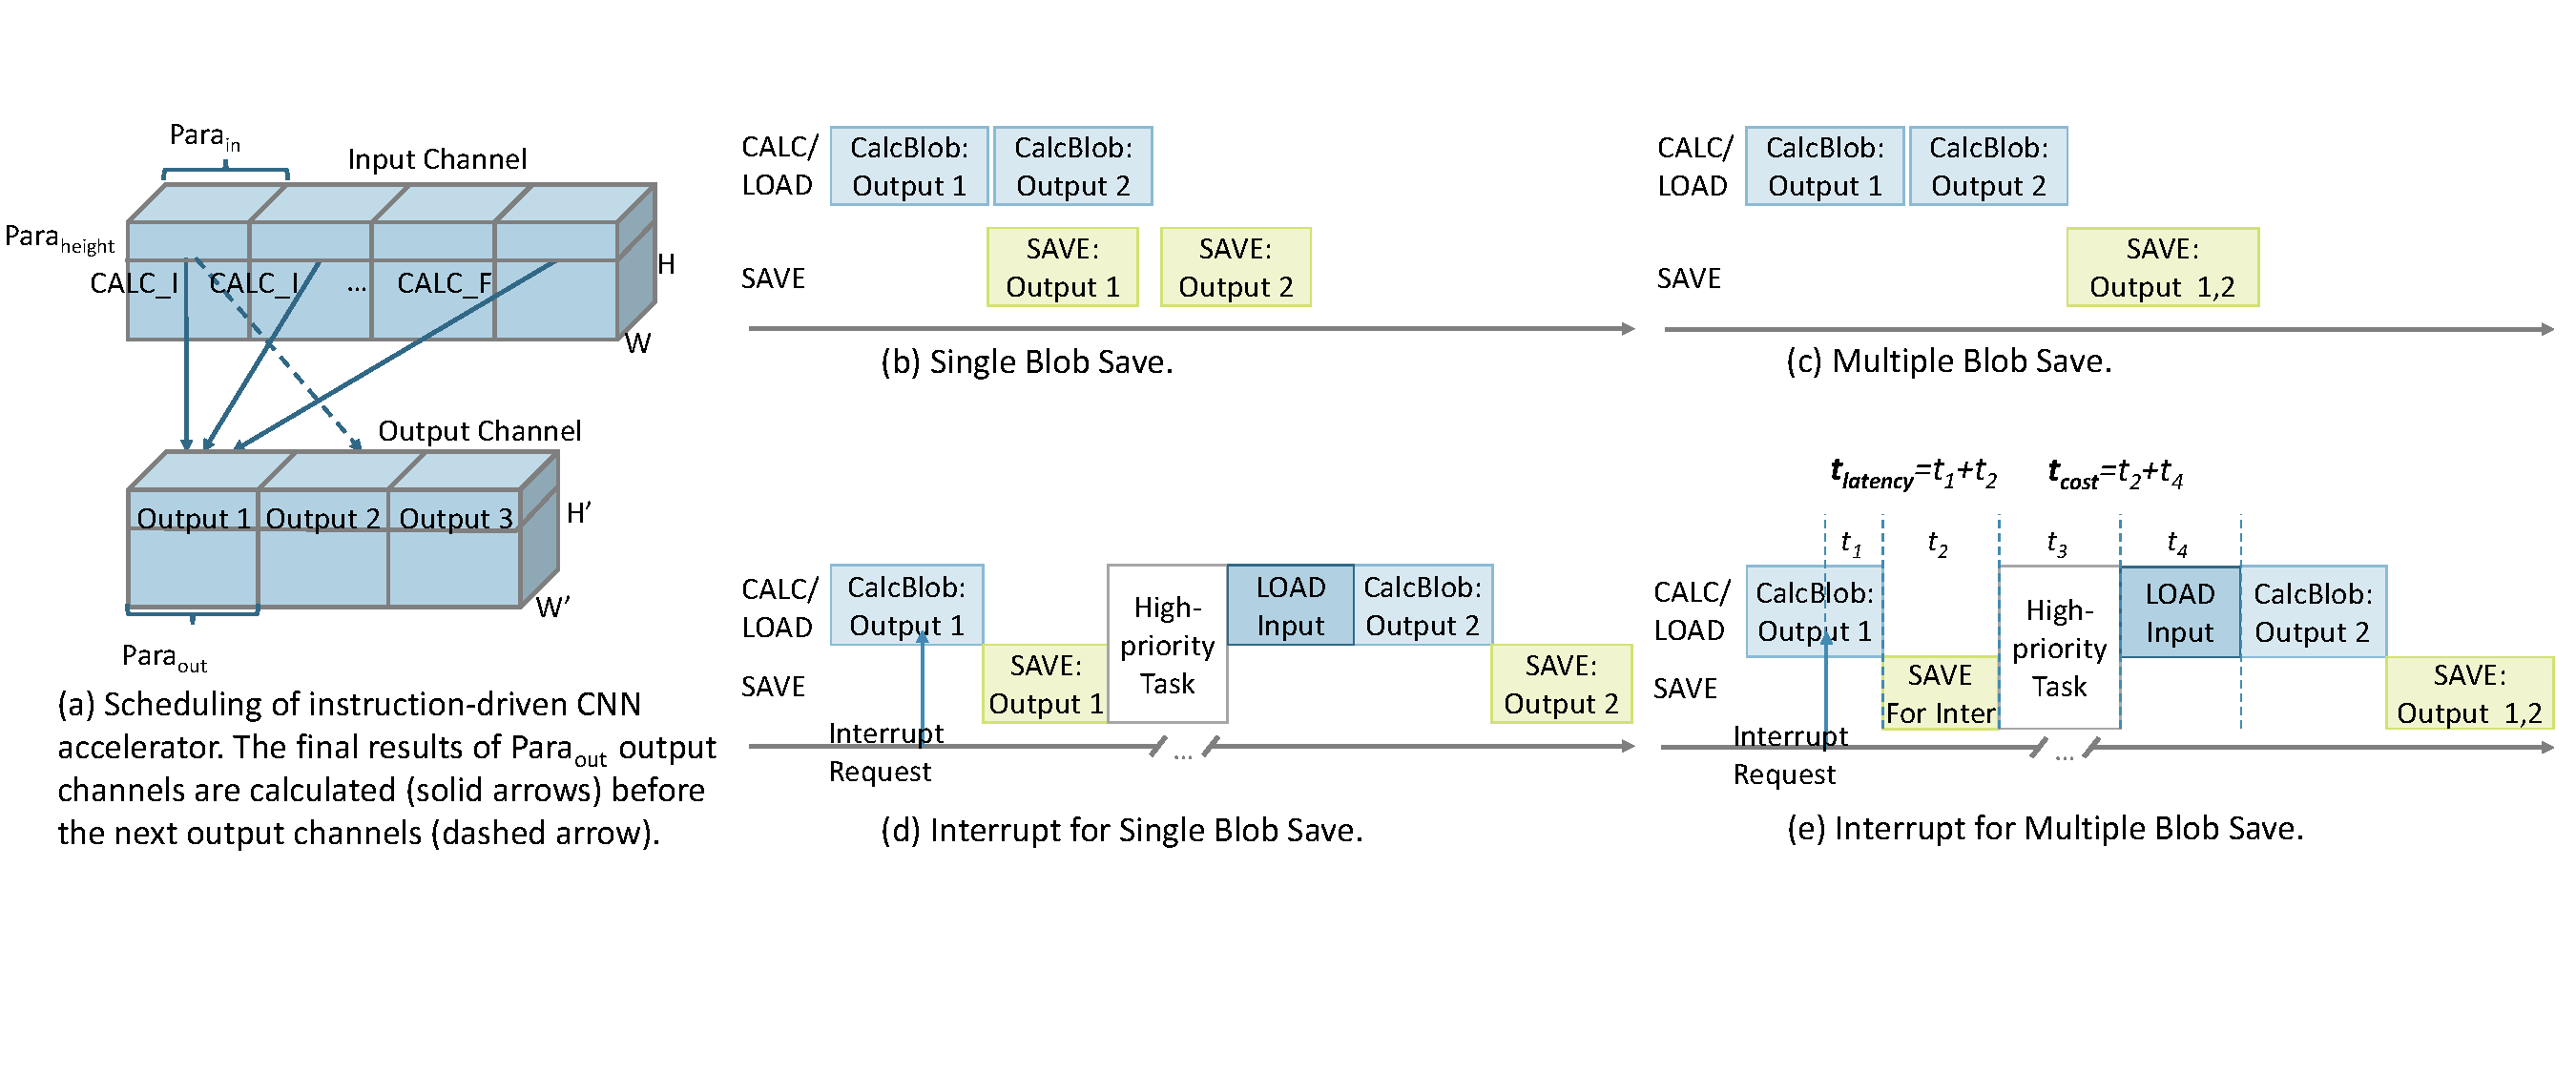
\includegraphics[width=0.99\textwidth]{fig/singlesave.pdf} 	
    \caption{
		Scheduling Illustration
    }
	\label{fig:singlesave}
\end{figure*}



\subsection{ Where To Interrupt: After SAVE/CALC\_F }
\label{sec:whereinter}
The virtual-instruction-based method has two potential factors that may lead to system performance degradation: 1) The extra data transfer to backup/restore running status takes up additional bandwidth resources. 2) The instruction fetching for the virtual instructions also uses bandwidth resources.
%  Even they are skipped and discarded.
To address the above problems of virtual-instruction-based method, we analyze the interrupt cost and select the positions of adding the virtual instructions.
The backup/recovery data for different interrupt positions at each kind of instruction are listed in the Backup/Recovery columns of \Cref{tab:instr}. The backup/recovery data transfer for each instruction is analyzed as follows:

\textbf{LOAD\_W / LOAD\_D. }
When an interruption occurs at LOAD, the newly loaded data are immediately flushed when running the high-level CNN, leading to bandwidth waste.

\textbf{CALC\_I.} 
When an interrupt occurs at CALC\_I, the unsaved final results ( generated by previous CALC\_F) should be saved to DDR. The intermediate data from current CALC\_I should also be sent to DDR for further use. At the Recovery stage, the intermediate data should be fetched from DDR. The data movement of intermediate results leads to additional bandwidth requirements.


\textbf{CALC\_F.}
When an interrupt occurs at CALC\_F, there are no intermediate results. 
Although it is necessary to back up the unsaved final results which are generated by previous CALC\_F, these results will be stored in DDR through the subsequent original SAVE instruction.
If the accelerator can record the interrupt status, we can modify the address and workload when executing subsequent original not-virtual save instruction.
In this way, we can avoid the repetitive transmission of the final output results.
% The state records and modifications to normal SAVE instruction will be introduced in the following subsections.
As introduced in \Cref{sec:howinter}, only the input data are shared across the CalcBlobs. Thus, the recovery virtual instruction only restores the shared input feature-maps.



\textbf{SAVE.}
The overhead of interrupt is only to transfer input data from DDR to the on-chip caches. 

In order to minimize the cost of interrupt, we make the CNN interruptible after the SAVE or CALC\_F. This method only introduces extra data transfer to recovery input data without any extra backup data. Thus, $t_{cost} = t_4$, in our virtual-instruction-based interrupt.

% Additional virtual instructions also take up bandwidth at instruction fetching phase, even if they are not executed. The instruction number of CALC\_I is tens of times of that of SAVE/CALC\_F. If the network can be interrupted after each CALC\_I, the rapidly increasing virtual instructions reduce the system performance.




\begin{figure}[t]
	\centering
    % \vspace{-0.1cm} 
    \setlength{\abovecaptionskip}{0cm} 
    \setlength{\belowcaptionskip}{-0.4cm} 
	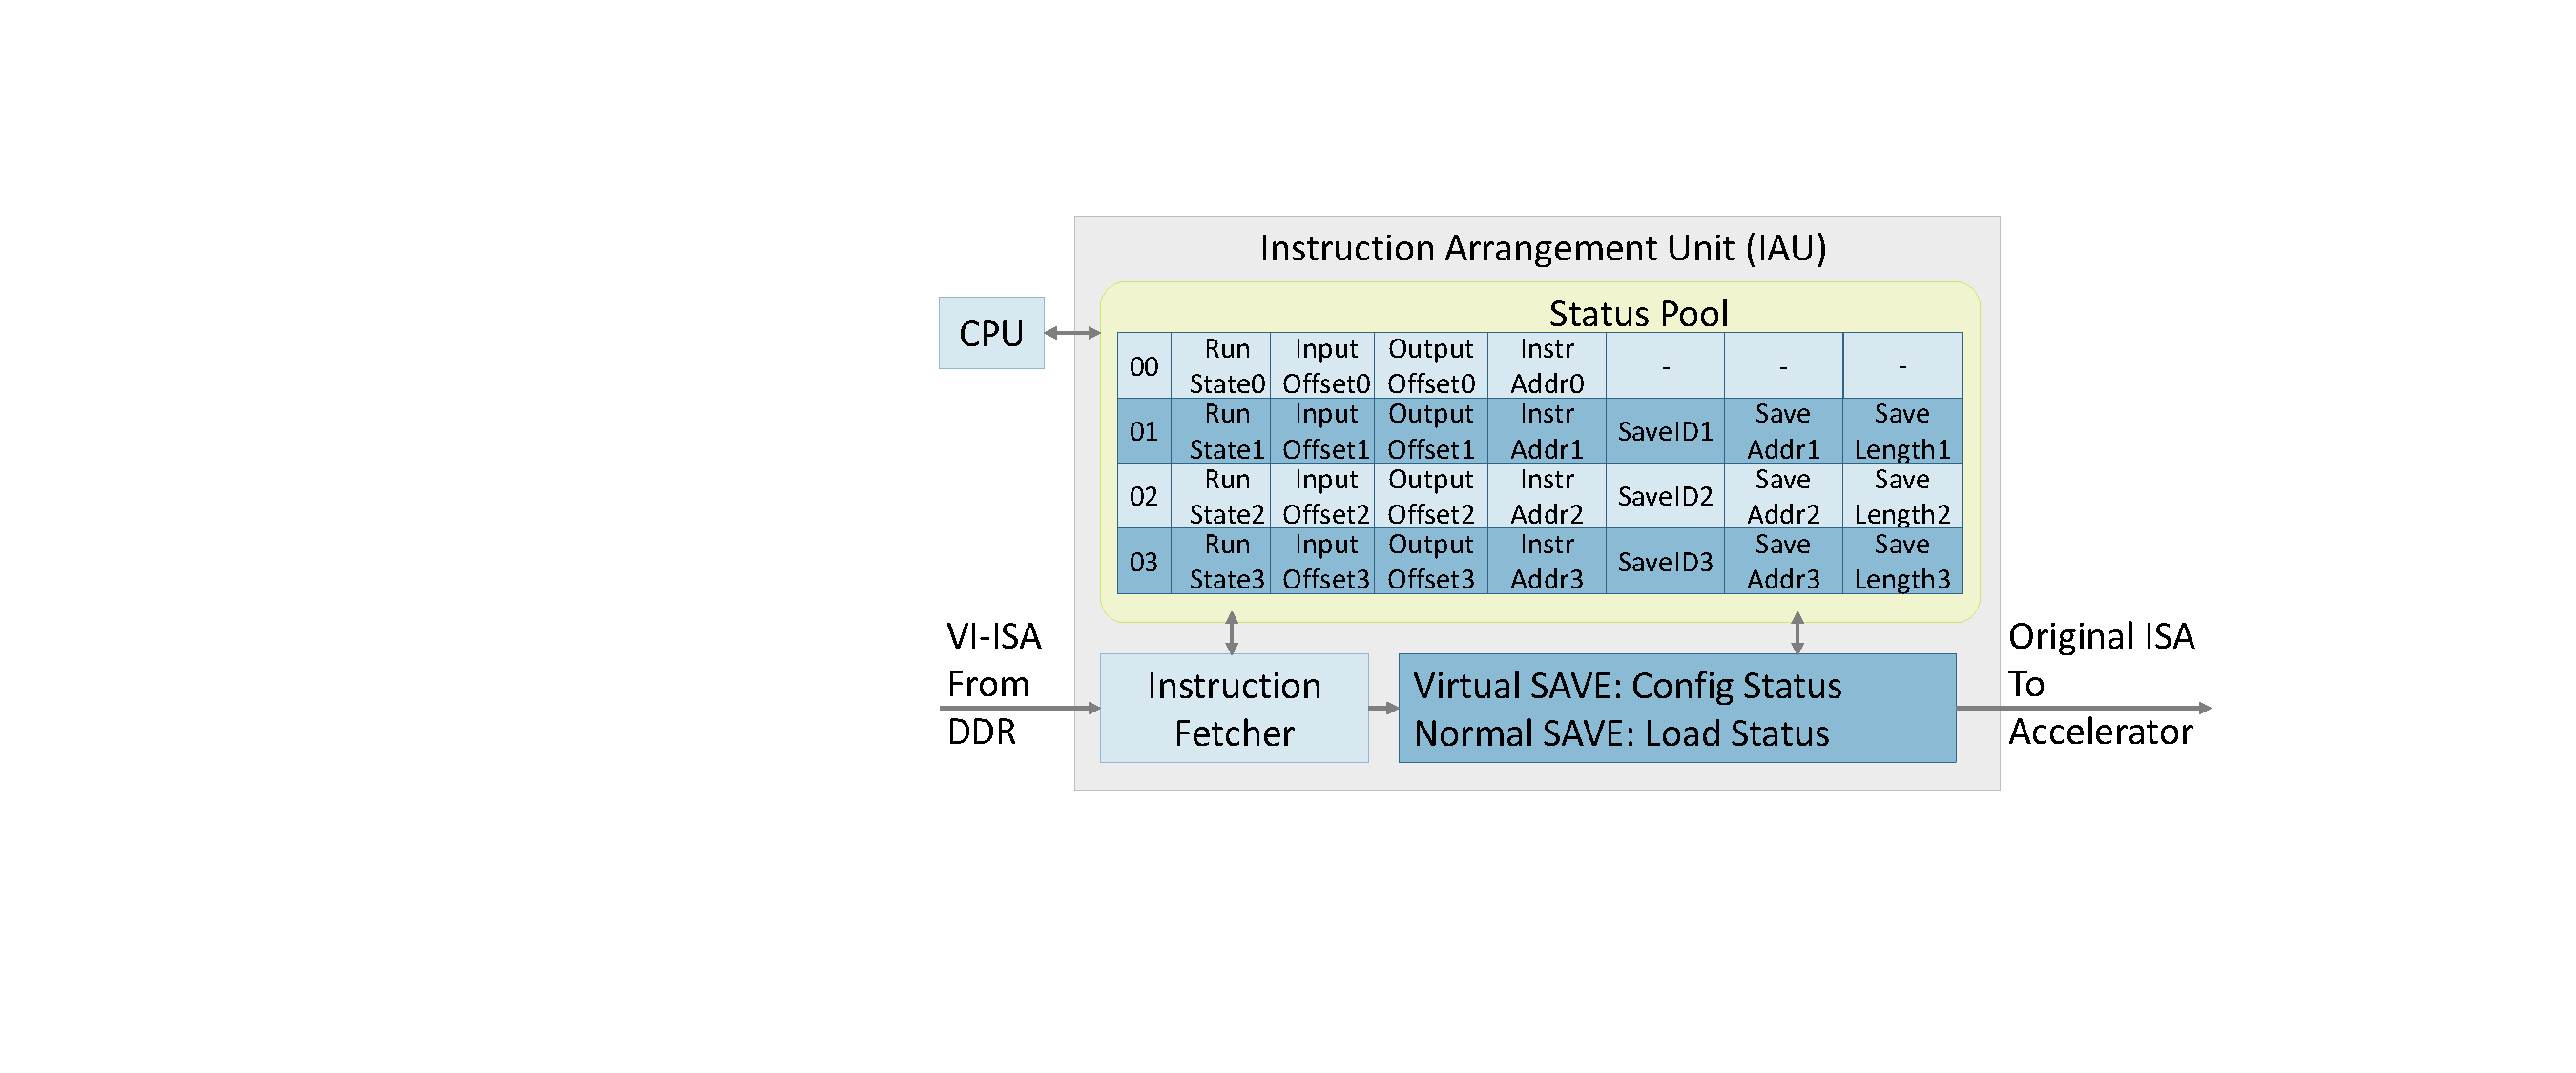
\includegraphics[width=0.99\linewidth]{fig/iau.pdf}
	\caption{Hardware architecture of IAU. 
	% The software on the CPU (PS side) communicates with IAU to access the CNN accelerator. IAU records the running state of each task. At runtime, IAU translates the input instruction sequence with virtual instructions to a normal sequence of instructions. IAU also modifies the normal SAVE instruction after interrupt occurs with the same SaveID, to avoid duplicate output data transfer. 
	}
	\label{fig:IAU}
\end{figure}
\begin{figure*}[t]
	\centering
    % \vspace{-0.1cm} 
    \setlength{\abovecaptionskip}{0cm} 
    % \setlength{\belowcaptionskip}{-0.05cm} 
	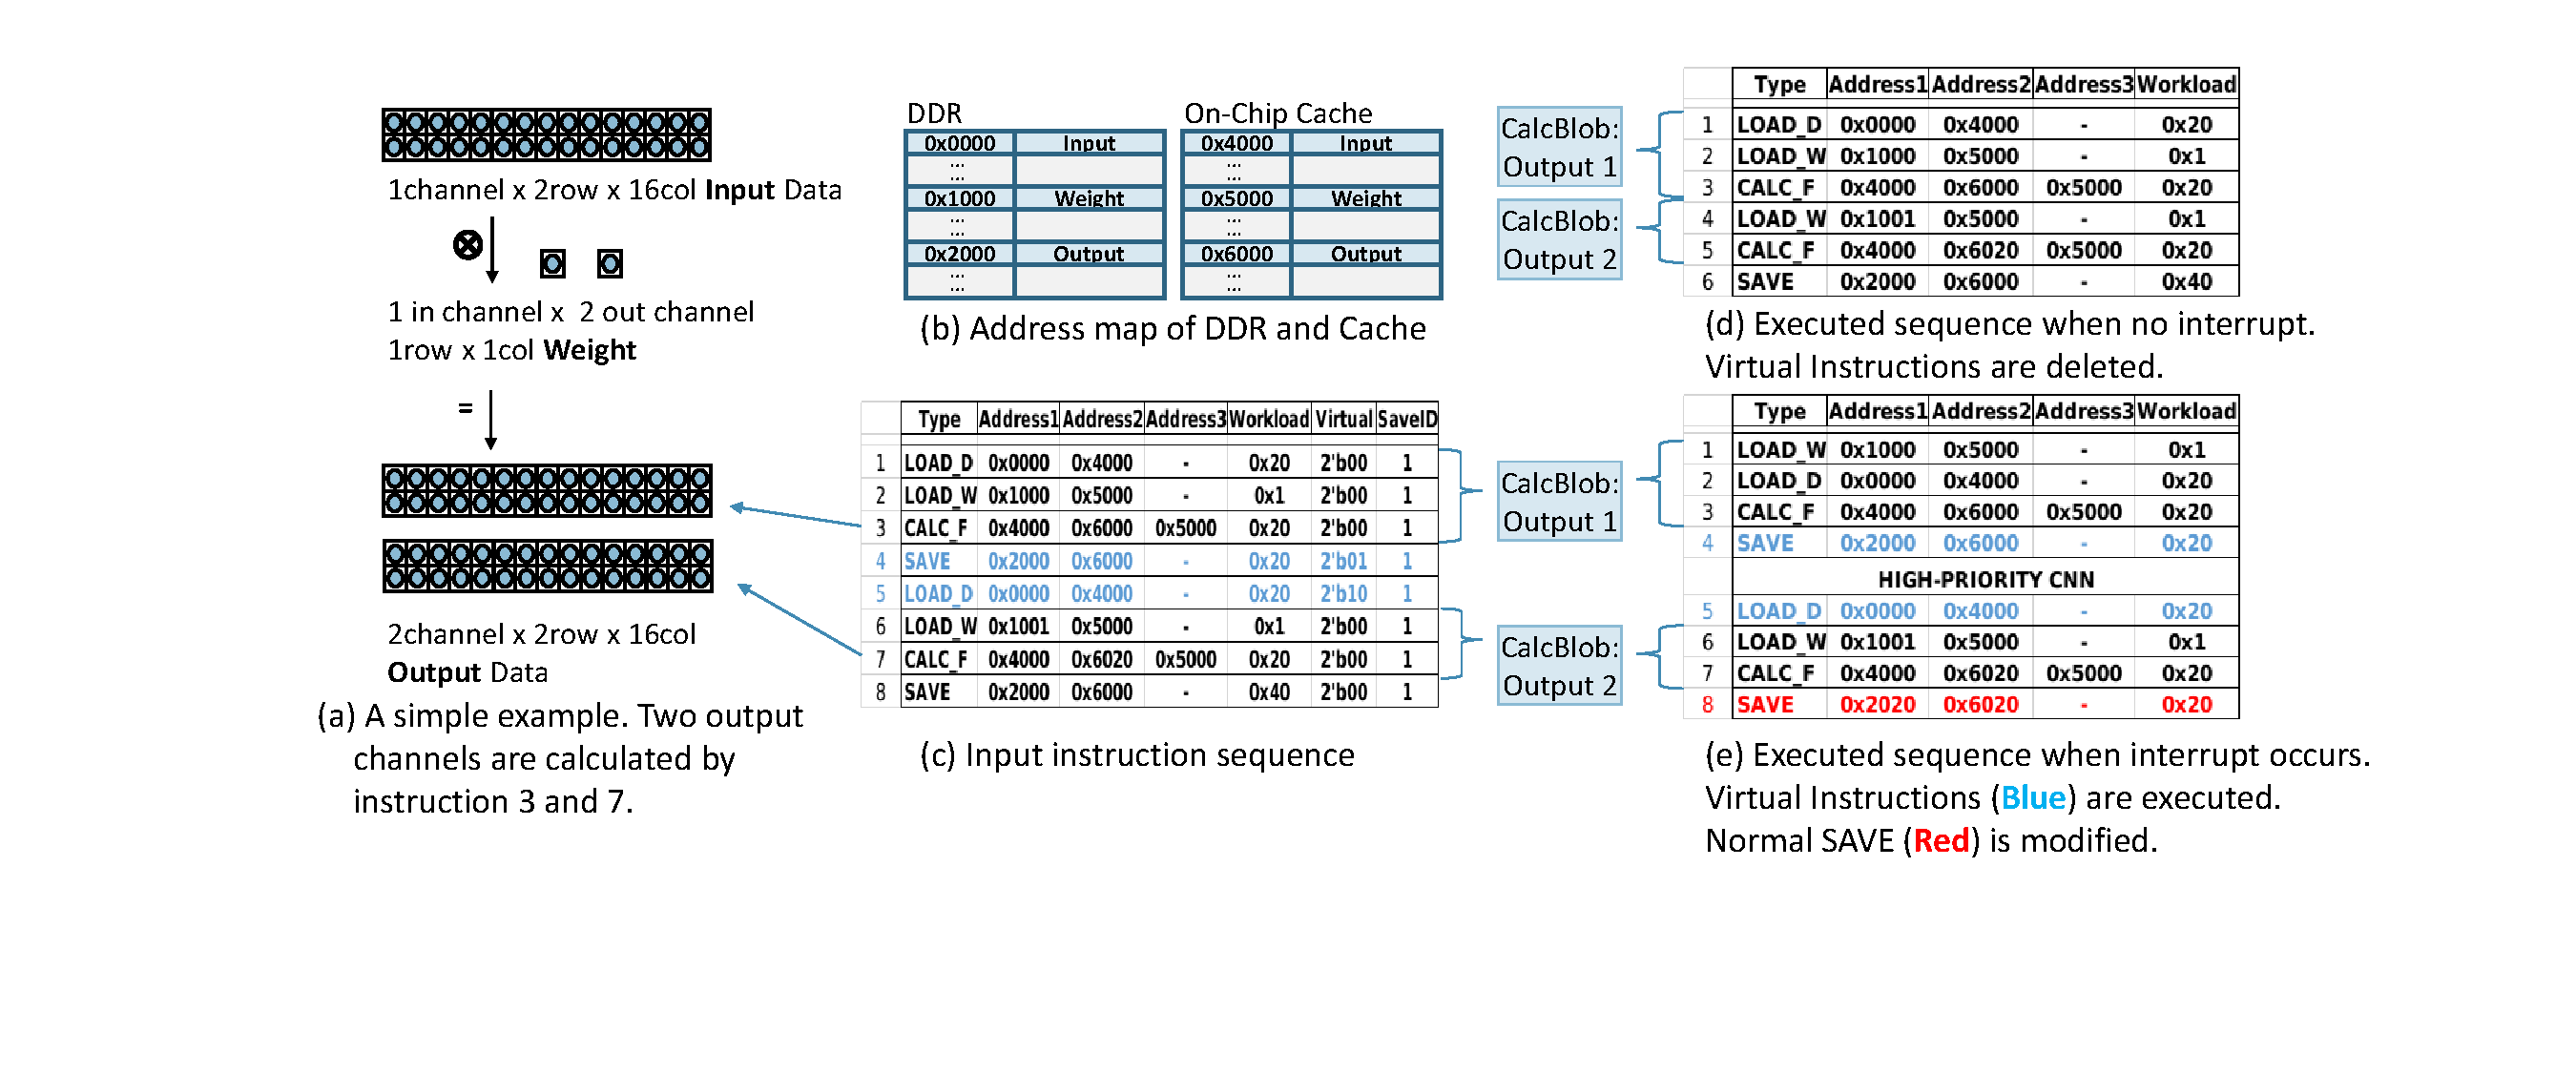
\includegraphics[width=0.99\linewidth]{fig/interexample.pdf}
	\caption{ A simple example of our proposed virtual-instruction-based interrupt. }
	\label{fig:interexample}
\end{figure*}


\subsection {Latency/Cost Analysis}

In this subsection, we quantitatively analyze the impact of interruptible position on latency and cost. 
As introduced in \Cref{sec:instrAcc}, ach CALC  instruction processes the convolution according to the hardware parallelism with $Para_{height}$ lines from $ Para_{in} $ input channels to $ Para_{out}$ output channels. 
We here note the computation of a CALC instruction an $instruction pulse$, or $pulse$.
The compuataion time of each pulse is related by the hardware architecture and the width of the convolution layer. The larger the width, the larger the workload of a single calculation instruction, and thus the CALC instruction consumes more time. We note the time consumption of a pulse as a function of the width of the featuremaps, $t_{pulse}$:

\begin{equation}
	t_{pulse}(W) = t_{Calc\_Hardware} \times W
\end{equation}

$t_{Calc\_Hardware}$ indicates the time for hardware to produce the intermediate results of one pixel, which is defined by the hardware design and the clock frequency. $W$ is the width of the featuremaps, indicating the workload of the instruction.

\Cref{fig:t1all} shows the worst case of waiting for finishing current operation of the Layer-By-Layer interrupt method. The worst case is that the interrupt request occurs at the beginning of the layer. At this case, the accelerator will wait untill finishing the whole layer. The calculation of the whole layer consists of $N_{pulse\_layer}$ successive CALC instructions. We note the worst time of waiting for finish the current layer, which is the total time of these pulses, as $t_{1\_layer}$.

\begin{equation}
	N_{pulse\_layer} = \frac{ Ch_{in} \times Ch_{out} \times H }{ (Para_{in} \times Para_{out} \times Para_{height}) } 
\end{equation}

\begin{equation}
t_{1\_layer} = N_{pulse} \times t_{pulse}(W)
\end{equation}

$Ch_{in}$ and $Ch_{in}$ is the number input channels and output channels. $H$ is the height of featuremaps.

On the other hand, if the execution of the CNN accelerator can be interrupted after SAVE/CALC\_F instructions, the worst case of waiting for finish current operation is illustrated in \Cref{fig:t1after}. The calculation of the whole CalcBlob consists of $N_{pulse\_VI}$ successive CALC instructions. We note the worst waiting time in this case as $t_{1\_VI}$.


\begin{equation}
	N_{pulse\_VI} = \frac{ Ch_{in} \times Para_{out} \times Para_{height} }{ (Para_{in} \times Para_{out} \times Para_{height}) } 
\end{equation}

\begin{equation}
t_{1\_VI} = N_{pulse\_VI} \times t_{pulse}(W)
\end{equation}

\begin{figure*}[htbp]
	\centering
	\subfigure[ $t_1$ for Layer-By-Layer method. ]{ \label{fig:t1all}
		\begin{minipage}[t]{0.45\linewidth}
			\centering
	\includegraphics[width=0.99\linewidth]{fig/t1all.pdf}
		\end{minipage}%
	}
	\subfigure[ $t_1$ for Virtual-Instruction method. ]{ \label{fig:t1after}
		\begin{minipage}[t]{0.45\linewidth}
			\centering
	\includegraphics[width=0.99\linewidth]{fig/t1after.pdf}
		\end{minipage}%
	}
	\label{fig:t1example}
	\caption{ Waiting time for finishing the current operation ($t_1$) in an example convolution layer. Compared with the Layer-By-Layer method, the waiting time of our Virtual-Instruction method is reduced to $1.6\%$ in this example. The reduction in latency is related to the height ($H$) of the input featuremaps.  }
\end{figure*}

Because our Virtual-Instruction method only interrupts the execution after CALC\_F and SAVE, there is no extra data transfer for the intermediate results. The backup operation in Virtual-Instruction method only transfers the final results, which are also transfered to DDR with the SAVE instructions in the Layer-By-Layer method. Experiment results shows that, the data transfer time for the final results is much less than the calculation time, in both Layer-By-Layer method and Virtual-Instruction method. Thus the latency to respond the interrupt request ($t_{latency}$) is mainly determined by the time of finishing current operation.

As the interrupt request is unpredictable, we model the interrupt location as evenly distributed within each layer. Thus the average interrupt latency is $\bar{t}_{latency} $.

\begin{equation}
	\bar{t}_{latency}  \simeq \frac{1}{2} \times t_{1}
\end{equation}

Compared with the Layer-By-Layer method, the latency of our method is reduced to $Rate_l$.

\begin{equation}
	\begin{split}
	Rate_l & =  \frac{\bar{t}_{latency\_VI}}{\bar{t}_{latency\_layer}} \simeq \frac{\frac{1}{2} \times t_{1\_VI}}{\frac{1}{2} \times t_{1\_layer}}  = \frac{ N_{pulse\_VI} \times t_{pulse}(W) }{ N_{pulse} \times t_{pulse}(W) }  \\
		   & = \frac{ N_{pulse\_VI} }{N_{pulse} } = \frac{ Ch_{in} \times Para_{out} \times Para_{height}  }{  Ch_{in} \times Ch_{out} \times H } \\
		   & = \frac{ Para_{out} \times Para_{height} }{ Ch_{out} \times H} 
	\end{split}
\end{equation}

$\bar{t}_{latency\_VI}$ and $\bar{t}_{latency\_VI}$ are the average interrupt latency of the Virtual-Instruction method and the Layer—By-Layer method. The effect of latency reduction of the VI method is related to the number of output channels ($Ch_{out}$) and featuremap height ($H$). The larger the featuremaps output channels and the height, the better  latency reduction result can be achieved.

An example of a convolution layer with a typical size in CNN is given in \Cref{fig:t1example}. The parameters are labeled in the figures. The latency can be reduced to $1.6\%$.


\subsection{Virtual Instruction ISA (VI-ISA) }
\label{sec:virtualinstr}

We add two fields to the instruction set: 1) Virtual and 2) SaveID, as illustrated in \Cref{fig:instructions}(b). 

\textbf{   Virtual Field}. The virtual instructions should be only valid when interrupt occurs. So we add a field in the original ISA, that indicates whether the instruction is a virtual instruction. If no interrupt occurs, virtual instructions will be skipped and discarded, which can ensure the efficiency of uninterrupted execution. Three values can be set to Virtual Field:
% \begin{itemize}

	\textit{2'b00} indicates this instruction is not virtual, should always be executed.
	
	\textit{2'b01} indicates this instruction is the SAVE instruction for backup. When an interrupt occurs, the high-priority network will start after this instruction.
	
	\textit{2'b10} indicates this instruction is the LOAD instruction for recovery. The corresponding instructions will be executed after the high-priority network.
% \end{itemize}

\textbf{ SaveID Field }
SaveID links CalcBlob instructions to the corresponding SAVE. SaveID of each not-virtual SAVE instruction differs. If the generated outputs of CalcBlobs are stored to DDR by a SAVE instruction, the CalcBlobs have the same SaveID as the SAVE instruction.

% The SaveID for a CalcBlob is the same as its CALC\_F instruction.
One SAVE instruction may correspond to one CalcBlob ( \textit{Single Blob Save}, illustrated in \Cref{fig:singlesave}(b) ) or multiple CalcBlobs (\textit{Multiple Blob Save}, illustrated in \Cref{fig:singlesave}(c)).

For Single Blob Save, no virtual SAVE is added. The high-priority network can be started after the original not-virtual SAVE. The virtual LOAD instructions for data recovery are generated after the original SAVE, and executed after the high-priority network. The execution timeline is shown in \Cref{fig:singlesave}(d).

For Multiple Blob Save, virtual SAVE and LOAD instructions are generated after the CALC\_F of each CalcBlob. When the interrupt request occurs, the virtual SAVE instruction will be executed before the start of the high-priority network. Virtual LOAD instructions for data recovery are executed after the high-priority network. The subsequent original not-virtual SAVE instruction with the same SaveID as the CalcBlob will be modified to avoid duplicate output data transfer. The execution timeline is shown in \Cref{fig:singlesave}(e).



\subsection{ Instruction Arrangement Unit (IAU) }

Instruction Arrangement Unit (IAU) is the hardware to handle the computing requirements from tasks with different priorities. The IAU monitors the interrupt status and generates the original ISA instruction sequence. The original CNN accelerator does not need to know the interrupt status, and only operates the instructions provided by IAU.

The hardware implementation of IAU is shown in \Cref{fig:IAU}, which supports four tasks with different priorities. Task 0 has the highest priority and is not interruptible. 
InstrAddr records the address to fetch the instructions of the corresponding task. The InputOffset and the OutputOffset, which indicate base address offsets of the input and output data, are configured by the software. 
SaveID, SaveAddr, and SaveLength record the status when an interrupt occurs. 
Subsequent not-virtual SAVE instructions will be modified according to the recorded interrupt status (SaveID, SaveAddr, and SaveLength), to avoid duplicate output data transfer.
% An example of the instruction modification will be given at \Cref{sec:exampleVirtual}.


\subsection{Example of Virtual Instruction}
\label{sec:exampleVirtual}


The example is based on a straightforward convolutional layer, which has only one input channel and two output channels. 
The convolution kernel size is $1 \times 1$. The shape of the input and output feature-maps is $ 2 \times 16 $ (\Cref{fig:interexample}(a)). The parallelism of the CALC instruction in this example is $ Para_{in} = 1$ , $ Para_{out}=1$ , $Para_{height}=2$.

Thus, the two output channels are calculated by two CALC\_F instructions ( instruction 3 and 7 in \Cref{fig:interexample}(c) ). The addresses used in the instruction example are listed in \Cref{fig:interexample}(b). \Cref{fig:interexample}(c) is the instruction sequence from DDR with VI-ISA. \Cref{fig:interexample}(d) is the executed original ISA instructions without interrupt. When an interrupt occurs at the first CalcBlob, \Cref{fig:interexample}(e) illustrates the backup/recovery instructions (Blue) and the modified SAVE instruction (Red). 
% IAU monitors the interrupt status and translates the VI-ISA instruction sequence to the original ISA instruction sequence.

% The hardware implementation of IAU is shouwn in \Cref{{fig:IAU}. There is a Status Pool which records the running states of each task. The InstrAddr is records the instruction address of each CNN

\section{Optimization For Post-Processing }
\label{sec:hardsoftcodesign}
\label{subsec:FEopt}

The high-priority feature-point extraction (FE) task is latency-sensitive and needs to be computed before the next picture arrives. With the help of the CNN accelerator, the latency of CNN backbone is reduced and the real-time requirement is satisfied. However, the post-processing of FE on the embedded CPU consumes more than 50ms, which becomes the bottleneck of the real-time system. In this section, the software and hardware acceleration for CNN-based FE method is introduced.



The flow path of our SuperPoint-based feature extraction method is shown in \Cref{fig:superpoint}. 
The CNN backbone of SuperPoint maps the input image $I\in \mathbb{R}^{H\times W}$ to a tensor $\mathcal{X}\in \mathbb{R}^{H_c\times W_c\times 65}$ for feature-point detection and to a tensor $\mathcal{D}\in \mathbb{R}^{H_c\times W_c\times D}$ for descriptors generation, where $H_c = H/8$ and $W_c = W/8$.
We optimize the software data flow of the components above, making them less computationally complex and more friendly to hardware. 

% As mentioned in \Cref{sec:relate}, there are two steps in the FE method: 1) feature-point detection and 2) feature descriptors generation. 
In SuperPoint  ~\cite{detone2018superpoint}, there are three components in the feature-point detector: 1) Softmax to generate confidence for each pixel. 2) Non-Maximum Suppression (NMS) to find the pixels with maximum confidence in its neighborhood. 3) Rank component to find out the first $k$ pixels with the highest confidence. 
In the feature descriptor generator, the normalization component consumes most of the computation. 


Then we design FPGA accelerators specifically for calculating softmax and normalization.

\subsection{Optimization of Feature-point Detection}
\label{sec:softmaxopt}

\begin{figure}[t]
    \centering  
    % \vspace{-0.1cm} 
    \setlength{\abovecaptionskip}{0cm} 
    % \setlength{\belowcaptionskip}{-0.05cm} 
    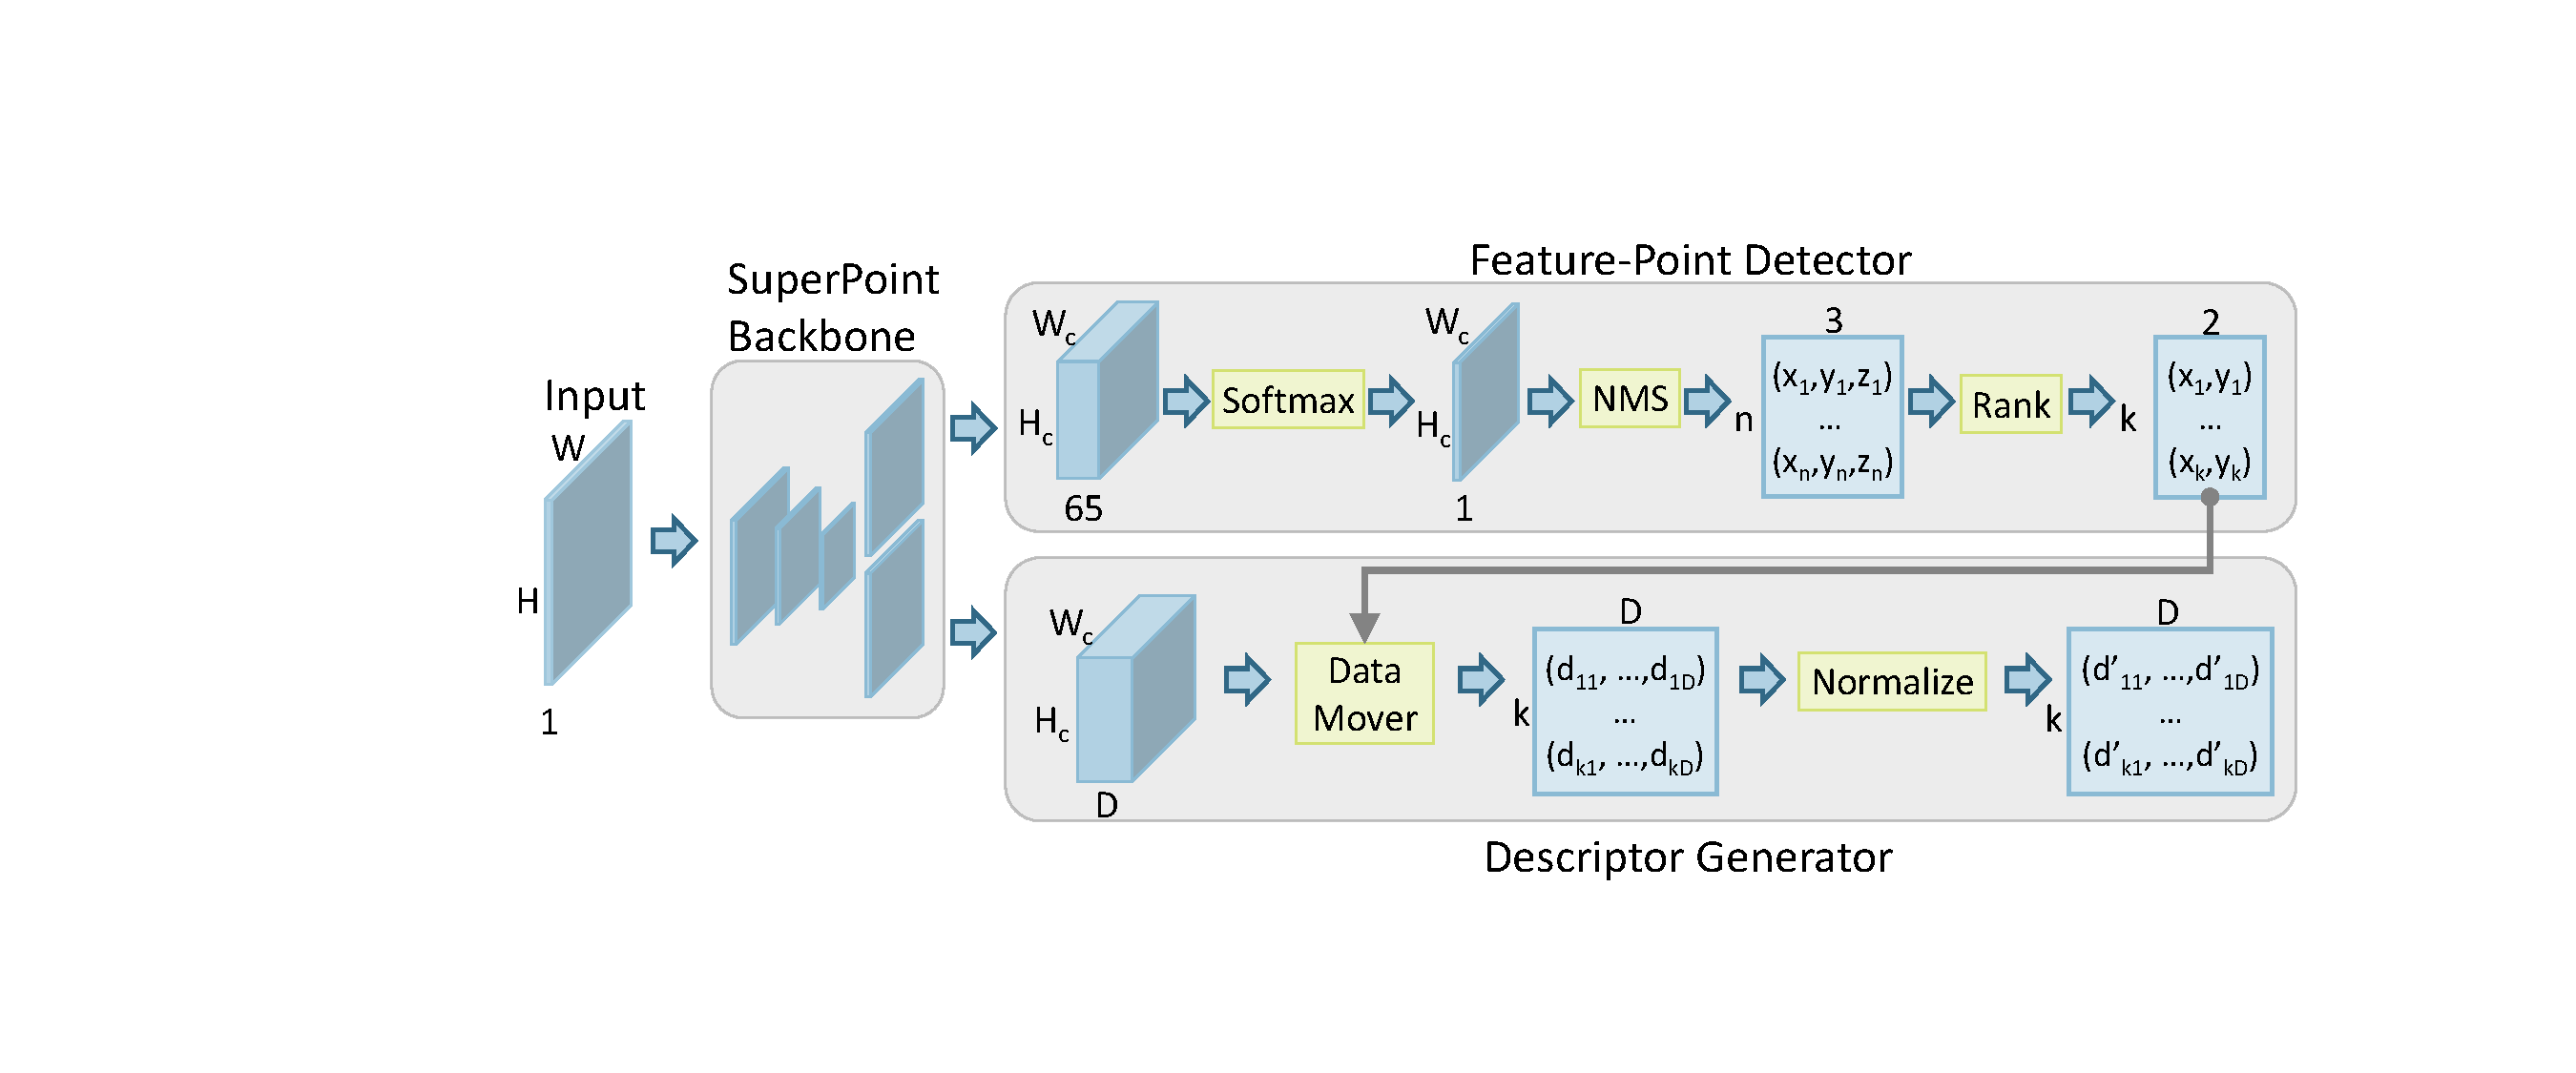
\includegraphics[width=0.99\linewidth]{fig/superpoint.pdf}
    \caption{Optimized feature extraction method based on SuperPoint}
    \label{fig:superpoint}
\end{figure}

\begin{figure}[t]
    \centering  
    % \vspace{-0.1cm} 
    \setlength{\abovecaptionskip}{0cm} 
    % \setlength{\belowcaptionskip}{-0.2cm} 
    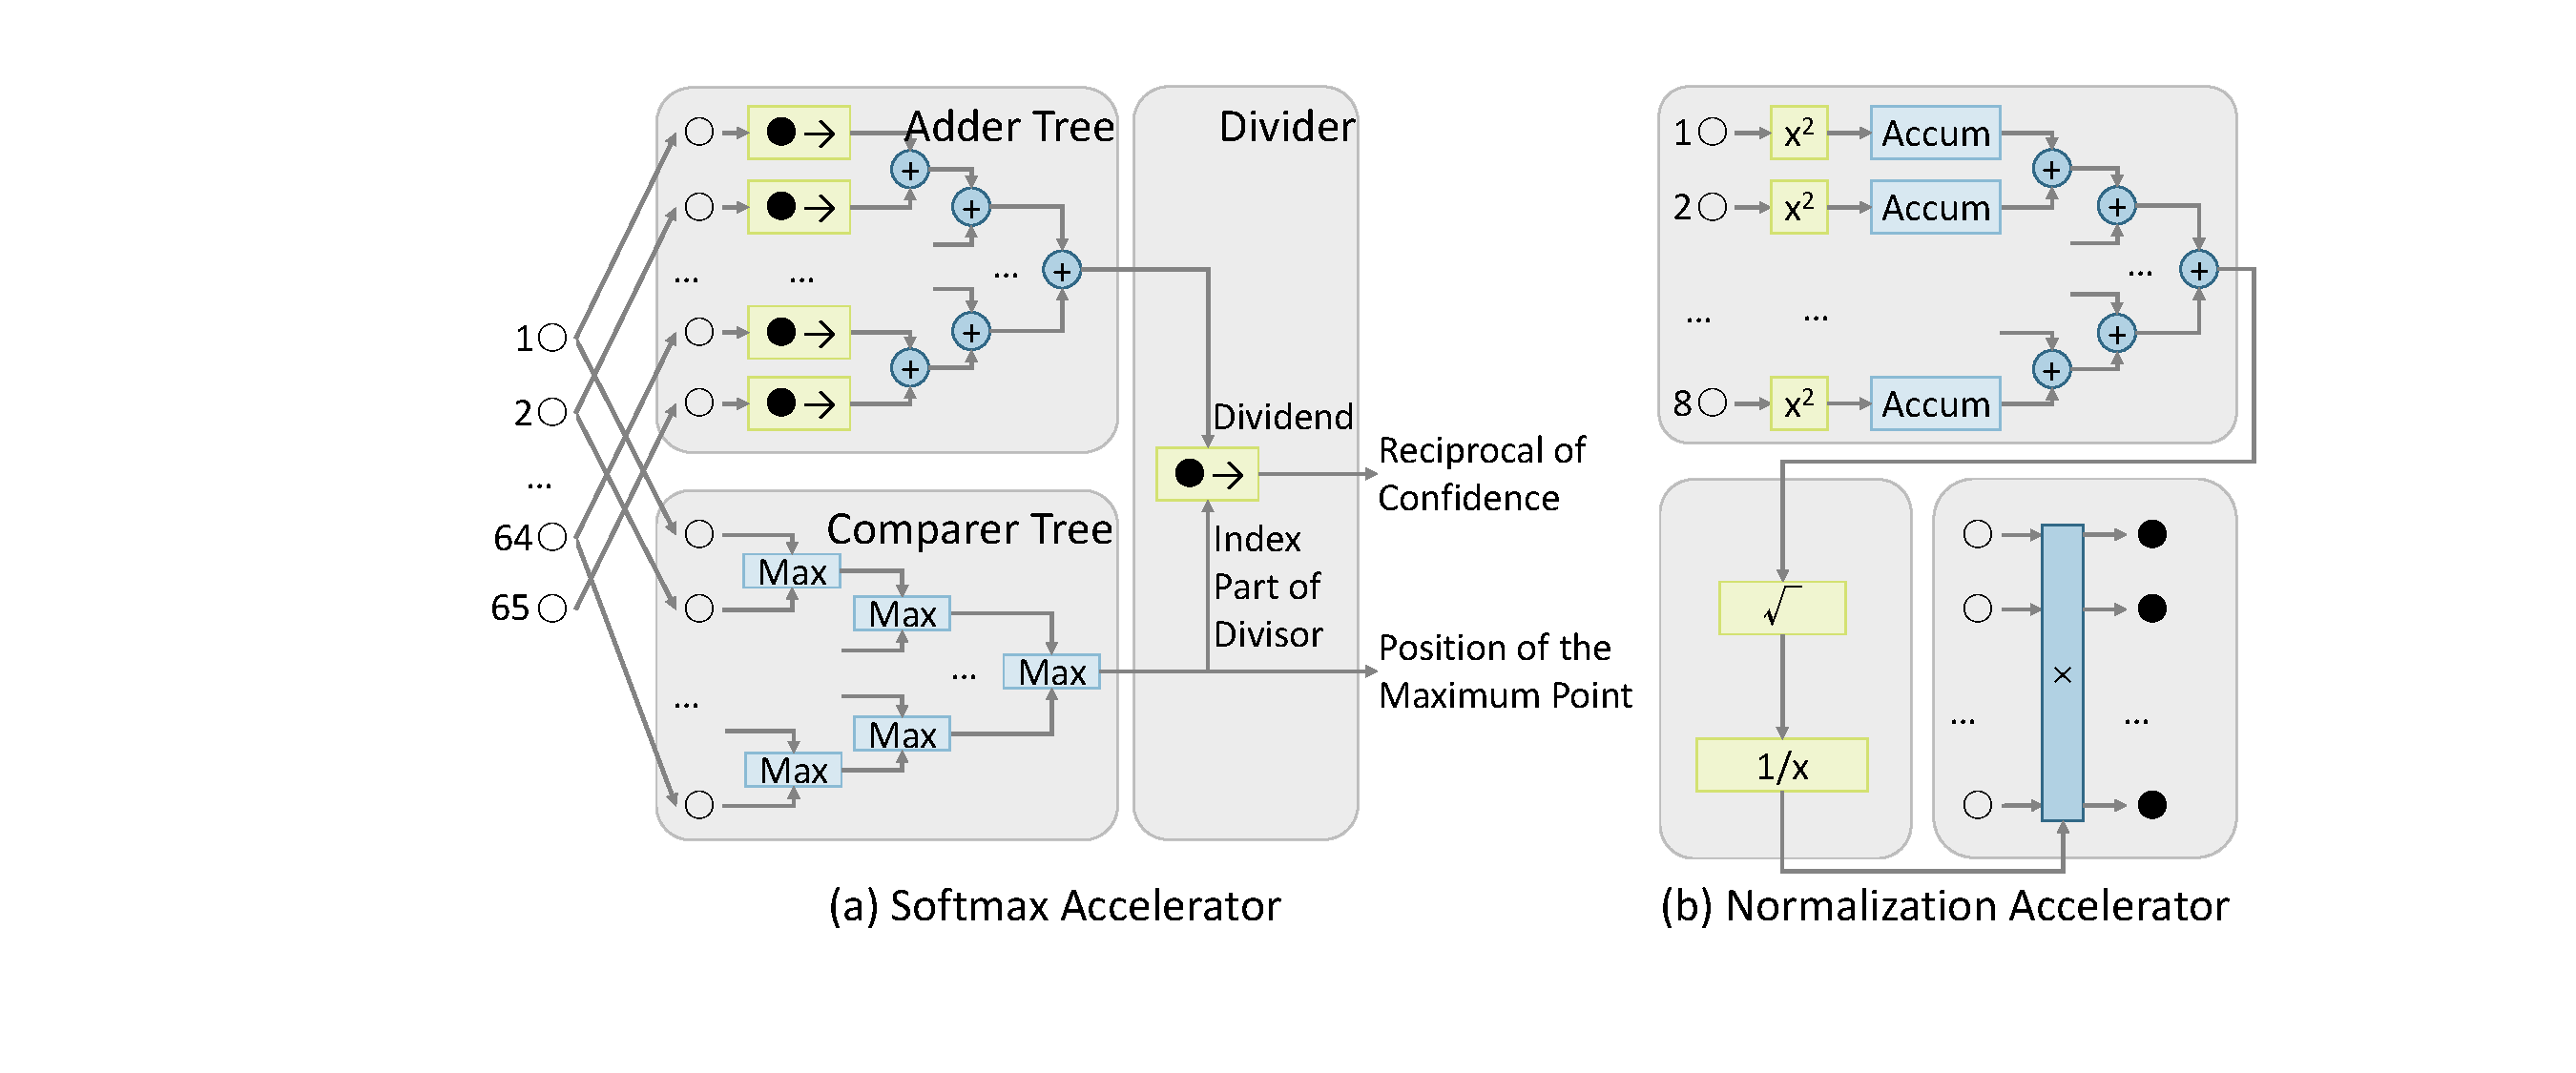
\includegraphics[width=0.99\linewidth]{fig/FEaccelerator.pdf}
    \caption{Hardware Architecture of FE Accelerators}
    \label{fig:FEaccelerator}
\end{figure}

For feature-point detection, the 65 channels correspond to local, non-overlapping $8 \times 8$ pixel grid areas plus a background channel. 
After a channel-wise softmax, the background channel is removed, and a $\mathbb{R}^{H_c\times W_c\times64}\Rightarrow \mathbb{R}^{H\times W}$ reshaping is performed. 
The channel-wise softmax makes the points in different grid areas have equal confidences.
The tensor of size $\mathbb{R}^{H\times W}$ corresponds to the confidences of the feature points in the input image.

The standard softmax function is defined as $\sigma (\mathbf {z} )_{i}$ in \Cref{equ:softmax_hard}.
We optimize the process of softmax that we only take the maximum value of each grid area for subsequent computations, which not only reduces the division operations of softmax but also simplifies the calculation of NMS and Rank.
We reduce the division operations and output size of softmax from $H \times W$ to $H_c \times W_c$.
The division operation is resource consuming on the FPGA platform. 
Our method can greatly reduce the number of divisions by $64 \times$, making it easy to accelerate softmax operation on FPGA.

\begin{equation}
    \sigma (\mathbf {z} )_{i}={\frac {e^{z_{i}}}{\sum _{j=1}^{K}e^{z_{j}}}}
    \Rightarrow
    \frac{1}{\sigma (\mathbf {z} )_{i}}={\frac {\sum _{j=1}^{K}2^{z_{j}}}{2^{z_{i}}}}{\text{ for }}i=1,\dotsc ,64;
    \label{equ:softmax_hard}
\end{equation}

Since the results of the softmax function are all positive, we can calculate the reciprocal of the softmax function ($\frac{1}{\sigma (\mathbf {z} )_{i}}$) in \Cref{equ:softmax_hard} as the normalized confidence, without affecting the results of the NMS and ranking process. We quantize the output feature map of CNN to 8-bit fixed-point number, i.e each $z_i$ in \Cref{equ:softmax_hard} is a 8-bit fixed-point number. We change the base of the power from $e$ to $2$ to make it more hardware friendly. Since the divisor is a power of $2$, we can also implement division by shift operation.

\Cref{fig:FEaccelerator}(a) shows an overview of the softmax module. It consists of three parts: adder tree, comparer tree and divider. Softmax reads 65 numbers from a grid region at once. Adder tree computes input to the power of $2$ using shift operation and calculates their sum. Comparer tree reads the values of the first 64 channels and returns the maximum value, as well as its channel number which contains the position information. The divider uses the shift operation to calculate the reciprocal of confidence.

NMS is applied to the detection to ensure that the feature-points are evenly distributed throughout the image. 
For each pixel in the original input image, NMS compares the confidence of this pixel with that of the pixels in a square neighborhood whose edge includes $\epsilon _{ori}$ pixels. 
If the confidence of the target central pixel is not the maximum in its neighbors, this point will be eliminated. 
The output of the NMS is a list of coordinates and confidences for each feature-point. 
Since the softmax optimization already gives the pixel with maximum confidence of each $8 \times 8$ block, the total number of pixels is reduced by $64 \times$ and the neighbors of each pixel is reduced by $10 \times$.
The total number of comparisons in NMS is reduced by $640\times$.

The ranking operation is to find out the top $k$ feature-points with maximum confidence after NMS. 
Since we only need to find feature-points without knowing their order, we create a heap of size $k$ to find the $k$ feature-points instead of quick sort ~\cite{Niu2012Top}.


% \subsection{NMS Optimization}

% Non-maximum suppression(NMS) is applied to the detection to help ensure that the feature-points are evenly distributed throughout the image. 
% For each pixel in the original input image, NMS compares the confidence of this pixel with that of the pixels in a square neighborhood whose edge including $\epsilon _{ori}$ pixels. 
% If the confidence of the target central pixel is not the maximum in its neighbors, this point will be eliminated from the valid feature-points. 
% The output of the NMS is a list of coordinates and confidences for each feature-point. 
% There are totally $H \times W$ points and the NMS does $\epsilon _{ori} ^ 2 - 1$ comparison operations for each points. 
% Thus, in the original NMS method, there are totally $H \times W \times (\epsilon _{ori} ^ 2 - 1)$ comparison operations.

% The softmax optimization introduced in \Cref{sec:softmaxopt} already gives the pixel with maximum confidence of each $8 \times 8$ block. Thus, we only need to compare each output pixel of softmax to the its adjacent blocks. The comparison area is a square box with an edge of $\epsilon _{opt}$ pixels. and $\epsilon _{opt} = 2\times \left \lceil (\epsilon _{ori}-1)/16 \right \rceil +1$. There are only $H_c \times W_c$ points. Thus, after NMS optimization, there are totally $H_c \times W_c \times (\epsilon _{opt} ^ 2 - 1)$ comparison operations.

% The $\epsilon _{ori}$ is set to 9 in the original implements SuperPoint, so $\epsilon _{opt} = 2\times \left \lceil (\epsilon _{ori}-1)/16 \right \rceil +1 = 3$. So that $H \times W \times 80 $ comparisons are done in the original NMS and we can do only $H_c \times W_c \times 8$ comparisons after optimization. The total number of comparisons is reduced by $640\times$.

% \subsection{Ranking Optimization}

% The ranking operation is to find out the top $k$ feature-points with maximum confidence. 
% The output is a list of coordinates for the $k$ feature-points. 
% In the original implementation, the confidence of all valid feature-points after NMS is sorted, and only the first $k$ feature points are used in the applications like SLAM and image matching. 
% There are $N_{nms}$ valid points after NMS. To sort all these $N_{nms}$ points, the time complexity is defined as:

% \begin{equation}
    % C_{sort} = O(N_{nms} \cdot log(N_{nms}))
    % \label{equ:csort}
% \end{equation}

% We create a heap of size $k$ and then look for the $k$ feature-points with the highest confidence. We do not compute the order of these $k$ points. The time complexity of the optimized ranking method is:

% \begin{equation}
    % C_{heap} = O(N_{nms} \cdot log(k))
    % \label{equ:optsort}
% \end{equation}

% In our expetiments, $N_{nms} \approx 2000$ and $k = 200$. The number of comparisons is reduced by $1.4\times$.

\subsection{Optimization of Descriptors Generation}

The input of the descriptor head sized $\mathbb{R}^{H_c\times W_c\times D}$ is semi-dense descriptor that each $8\times8$ pixel cell has a descriptor. In the original implementation, a bicubic interpolation and normalization yields fine descriptors of size $\mathbb{R}^{H\times W\times D}$. Then, according to the result after ranking, the descriptors corresponding to the k feature points are combined into a list and output. After maximum point softmax, each $8\times8$ cell contains at most one valid feature-point. So we can use semi-dense descriptor as the dense descriptor of the potential feature-point and do not need bicubic interpolation.




The number of descriptors that need to be normalized has been reduced from $H\times W$ to $H_c\times W_c$. In addition, we normalize the descriptors after sorting the feature-points, which means we only need to normalize $k$ descriptors. If we set $H=480$, $W=640$ and $k=200$, then the computational complexity of the normalization process will be reduced by $1500\times$. However, $k$ descriptors are not stored in contiguous memory space. We use a data mover to move data from discrete address spaces.

The architecture of normalization accelerator is illustrated in \Cref{fig:FEaccelerator}(b). The normalization module can read 8 numbers per clock cycle. The normalization process is divided into three stages and requires each descriptor to be read twice. In the first stage, we compute the sum of the squares of the descriptors, which takes 32 clock cycles when $D=256$. Then the reciprocal of square root of sum is computed as the normalization coefficient. In the final stage, the descriptor is read a second time and multiplied by the normalization coefficient.

% \subsection{Optimization for PR Post-Processing}

% \begin{figure}[t]
%     \centering
%     \includegraphics[width=1\linewidth]{fig/pr.eps}
%     \caption{The architecture of GeM network}
%     \label{fig:gem}
% \end{figure}

% Figure \ref{fig:gem} shows the data flow of GeM network  ~\cite{gem} for PR. The CNN backbone of GeM is a resnet101 network without the last two layers(pooling and FC). The CNN maps the input image $ I \in \mathbb{R}^{3 \times H \times W}$ to a tensor $\mathcal{X} \in \mathbb{R}^{C \times H_1 \times W_1}$. Here, the channel number $C = 2048$. Then the gem pooling layer pool the tensor into a vector $\mathcal{V} \in \mathbb{R}^{C}$. (To avoid ambiguity, we use "GeM" to represent the whole network and "gem" to represent the pooling layer only.) Finally, the vector is normalized. After that, we use dot product or L2 distance of the vectors to calculate similarity of places. Because feature extraction needs to be real-time and is time consuming, we modify its software utilization and design FPGA accelertor for this process.

% Experiments show that the post processing (gem pooling and normalization) consume nearly twice the time as CNN network does. After optimization, we can reduce time to 1/? of that of origin.

% \subsubsection{GeM Pooling Optimization}

% The element of the vector $\mathcal{V}$ is calculated by

% \begin{equation}
%     \mathcal{V}_i = (\sum_{x \in \mathcal{C}_i} x^p)^{1/p}, i=1, 2, ..., 2048.
% \end{equation}

% Here, the parameter $p$ is learned by back propagation and is set to 2.9? in original paper. To make it friendly for hardware computation, we change it to $p=3$. In this way, the power computation can be converted to multiplication computation. This will save a lot of time and calculation resources on FPGA without loss of accuracy. We notice that the channels are independent with each other, so it's convenient to do parallel computation on FPGA. With Vivado HLS tool, we design an IP core for gem pooling and efficiently reduce time.

% \subsubsection{Normalization Optimization}

\section{Evaluation and Results}
\label{sec:experiments}


\begin{figure*}[t]
  \centering
%   \vspace{-0.1cm} 
  % \setlength{\abovecaptionskip}{0cm} 
%   \setlength{\belowcaptionskip}{-0.05cm} 
  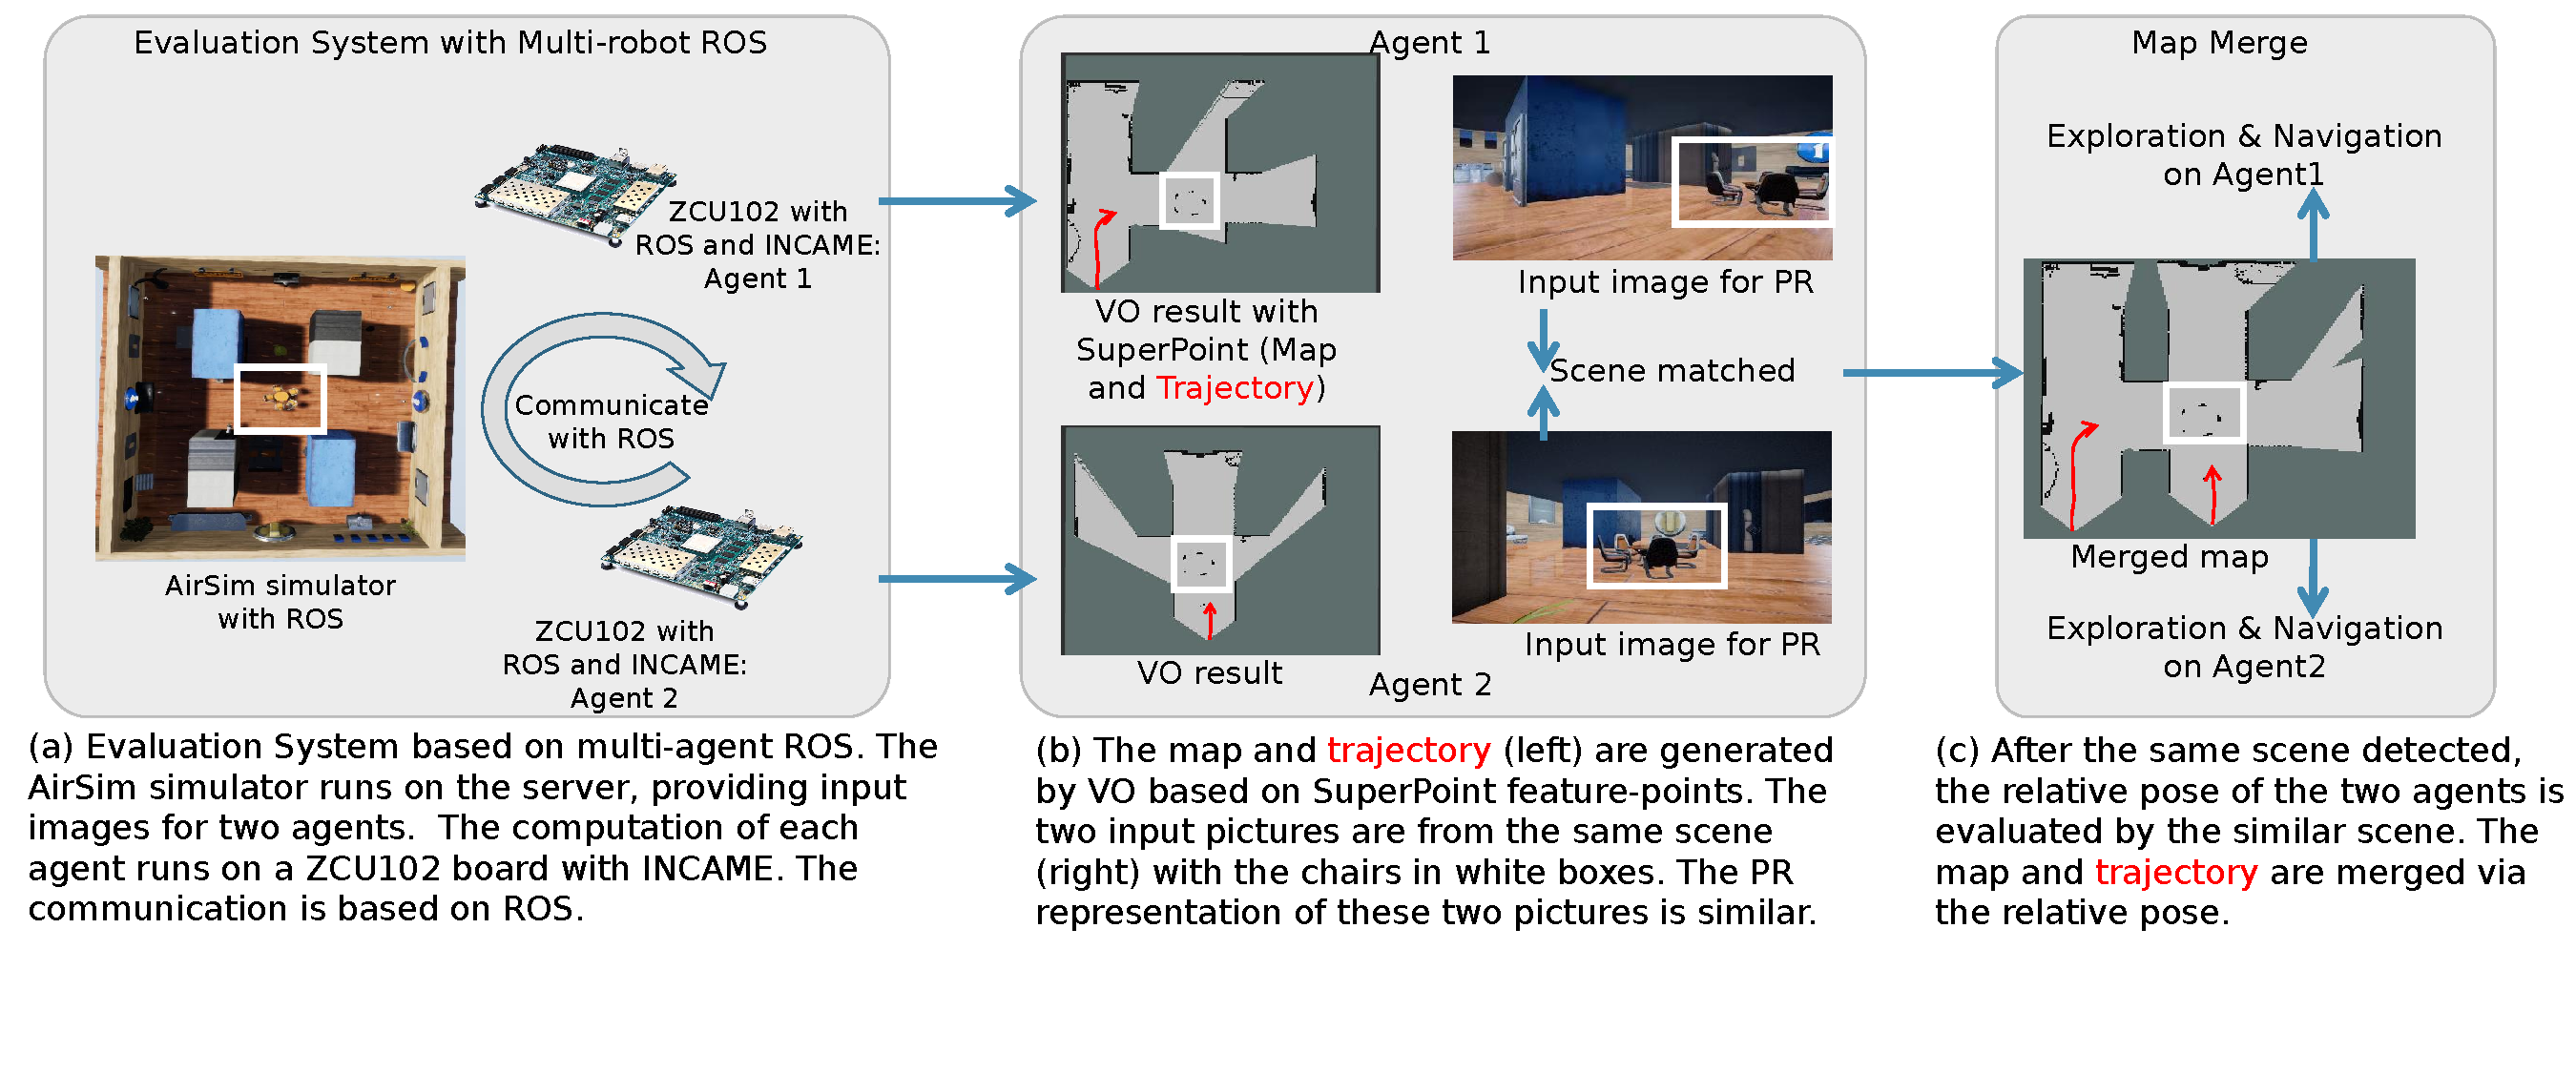
\includegraphics[width=0.99\linewidth]{fig/env.pdf}
  \caption{Multi-robot exploration: environment and results. }
  \label{fig:env}
\end{figure*}


% In this section, the evaluation of the instruction-based-interruption, hardware modules for FE post-processing, and the overall MR-Exploration system are presented and analyzed.



\subsection{ Experiment Setup }

The hardware-in-loop evaluate environment is illustrated in \Cref{fig:env}(a). There is a simulation server providing the simulation environment based on AirSim  ~\cite{shah2018airsim}, which is a high-fidelity visual and physical simulation for autonomous vehicles. The AirSim simulation server provides the camera data for each agent. Two Xilinx ZCU102 boards  ~\cite{zcu102}, with ZU9 MPSoC  ~\cite{MPSoC}, are responsible for the calculation of each agent. 
The components in \Cref{fig:maexp} for each agent are implemented in the ZCU102 board. The implementation of the FE (\textcircled{1} in \Cref{fig:maexp}), SuperPoint ~\cite{detone2018superpoint}), are introduced in former sections. GeM  ~\cite{radenovic2018fine} is used to implement the PR module (\textcircled{2}). GeM is a CNN-based method with ResNet101 \cite{he2016deep} as the backbone, and the post-processing of GeM calculates the 3-norm of the output featuremaps.
The VO module (\textcircled{3}) in the experiment is the PnP  ~\cite{LepetitMoreno-Noguer-EPnP} method, which is widely used in the feature-point based VO. 
% including the open source the ORB-SLAM  ~\cite{Mur-Artal:2017281}. 
The DOpt module (\textcircled{4}) is proposed in  ~\cite{Choudhary:2017e66} and also used in former distributed SLAM system ~\cite{cieslewski2018data}. 
The Map Merging  ~\cite{Andre2014} (\textcircled{5}), Exploration  ~\cite{8202319} (\textcircled{6}), and Navigation  ~\cite{tbd} (\textcircled{7}) in this work are provided by the ROS framework. 

The hardware resources are listed in \Cref{tab:hardware}. The CNN backbone is calculated by the Angel-Eye CNN accelerator ~\cite{guo2017angel} on the FPGA side of ZCU102 (Programmable logic, PL side). The FE post-processing steps run on our proposed accelerators, also on the PL side. The PL side has 2 clock frequencies. The CNN accelerator and the IAU are running at 300MHz. The accelerator for FE post-processing is running at 200MHz. Compared with the CNN accelerator, IAU and FE post-processing use very little hardware resources.

% Table generated by Excel2LaTeX from sheet 'Sheet1'
\begin{table}[t]
  \centering
  % \setlength{\abovecaptionskip}{2pt}
  \caption{Hardware consumption of the proposed hardware}
% Table generated by Excel2LaTeX from sheet 'Sheet1'
\begin{tabular}{|c|c|c|c|c|}
  \hline
        & $\# DSP$ & $\# LUT$ & $\# FF$ & $\# BRAM$ \\
  \hline
  On-Board resource &   2520   &  274080      &  548160     & 912 \\
  \hline
  CNN accelerator &   1282   &  74569      &   171416    & 499 \\
  \hline
  IAU &   0   &  2268      &   4633    & 4 \\
  \hline
  FE post-processing & 25      &  17573     &   29115    & 10 \\
  \hline
  \end{tabular}%
  
  \label{tab:hardware}%
\end{table}%


\subsection{Virtual Instruction-based interrupt }

\subsubsection{ Interrupt response latency and extra cost}


We evaluate the latency to respond the interrupt and the performance degradation of different interrupt method. In MR-Exploration, only the low-priority PR task is interruptible, and the interrupt position is unpredictable. GeM  ~\cite{radenovic2018fine} is used to implement the PR module in the experiment.
The CNN backbone of the GeM is ResNet101  ~\cite{he2016deep}, which contains 101 convolution layers. The input shape of the CNN is $480 \times 640 \times 3$. The parallelism of the Angel-Eye is $Para_{height}=8$, $Para_{in}=16$, $Para_{out}=16$, i.e. each CALC instruction processes 8 lines from 16 input channels to 16 output channels. 
% Thus, we randomly selected some interrupt locations inside the PR network.

As shown in \Cref{fig:scatter1024}(a), the latency to respond the interrupt in CPU-like method consists of the time to finish current executing instruction and the data backup time ($t_{latency} = t_1+t_2$) for the on-chip data/weights caches (totally 2.2MB). The latency in layer-by-layer interrupt is the time to finish current layer. The latency of our virtual-instruction-based method is the time to finish current executing instruction and the backup time for the calculated output results. 

The cost of CPU-like interrupt is the data transfer time of all the on-chip caches (totally 2.2MB) to/from DDR ($t_{cost} = t_2+t_4$). The cost of virtual-instruction-based method is only the recovery of the input/weights from DDR to on-chip caches ($t_{cost} = t_4$). There is no extra cost for the layer-by-layer interrupt.

% For a precise evaluation the CNN run time, we record the clock cycles of the beginning and end of each instruction. The time of the interrupt response latency and the total cost in the following evaluation is calculated from the clock cycles and the clock frequence.


We randomly sample 12 positions of the ResNet101 CNN backbone. The interrupt response latency and the extra time cost for different implementation of interrupt at the positions are listed in \Cref{fig:scatter1024}(b).
The CPU-like interrupt consumes the most extra cost ($t_{cost}$). Though the layer-by-layer interrupt consumes no extra time, the latency is much higher than our virtual-instruction-based interrupt. 
This is because the layer-by-layer interrupt need to wait for completion of a layer. The performance at same interrupt position in our proposed virtual interrupt can interrupt inside a layer, with lower latency.

Furthermore, though the network structures differ between different CNNs, the convolutional layers, which are the basic component in CNN, are similar between different CNNs. INCAME monitors the running status inside each layer, and the interrupt respond latency and extra cost are only relevant to the currently operating layer. Thus, the latency and cost are also similar between different CNNs. In conclusion, the process for different CNN tasks are similar, and the cost of different tasks are similar.

\subsubsection{ Time comparison between $t_1$ and $t_2$ }

As described in \Cref{sec:virtualinstr}, the Layer-By-Layer interrupt method do not need to backup data before interruption ($t_2 = 0$). Though our Virtual-Instruction method (VI method) need to spend time to backup the final results, which are already generated yet not stored to DDR ($t_2$). However, compared with computation, the time of data backup is very short. We list the backup time and the convolution time at some of the interrupt position in \Cref{fig:scatter1024}(b), with different featuremap shape, kernal size, and input/output channels. $H$, $W$ are the height, width of input featuremaps. $Ch_{in}$, $Ch_{out}$ are the number of input and output channels. The time of backup and calculation is listed in $Backup$ and $Conv$ columns. The ratio of backup and calculation are listed in the last column. The backup operation only consumes less than 20\% of the calculation time. For the first layer (first line of \Cref{tab:timecompare}). The input channels number is too small so the calculation time is also very short. Therefore, the backup time has reached half of the calculation time. 

% Table generated by Excel2LaTeX from sheet 'Sheet4'
\begin{table}[t]
  \centering
  % \footnotesize
  \caption{Time comparison between data backup and calculation}
    \begin{tabular}{|c|c|c|c|c|c|c|c|}
    \hline
    \multirow{2}[2]{*}{$H$} & \multirow{2}[2]{*}{$W$} & \multirow{2}[2]{*}{$Ch_{in}$} & \multirow{2}[2]{*}{$Ch_{out}$} & Kernel & Backup & Conv  & \multirow{2}[2]{*}{$\frac{Backup}{Conv}$} \bigstrut[t]\\
          &       &       &       & Size  & (us)  & (us)  &  \\
    \hline
    480   & 640   & 3     & 64    & $7 \times 7$ & 26.29  & 52.38  & 50.2\% \\
    \hline
    120   & 160   & 128   & 128   & $3 \times 3$ & 8.77  & 41.18  & 21.3\% \\
    \hline
    30    & 40    & 1024  & 2048  & $1 \times 1$ & 1.25  & 8.75  & 14.3\% \\
    \hline
    30    & 40    & 512   & 512   & $3 \times 3$ & 1.42  & 39.36  & 3.6\% \\
    \hline
    16    & 20    & 512   & 512   & $3 \times 3$ & 0.75  & 20.16  & 3.8\% \\
    \hline
    \end{tabular}%
  \label{tab:timecompare}%
\end{table}%




\subsubsection{ Additional data transfer for the virtual instructions. }
% The worst latency of the layer-by-layer interrupt reaches 10 ms, because the interrupt occurs at the beginning of the second layer, which is the most time-consuming layer (10ms). The layer-by-layer interrupt need to wait for the finish of this layer. The performance at same interrupt position in our proposed virtual interrupt is not significantly different from that of other positions. Our method is significantly better than others at worst case. 

The extra virtual instruction number is listed in \Cref{tab:instrnum}. Compared to the normal instruction transfer, the volume of virtual instructions is less than 10\%. The performance degradation brought by the extra virtual instructions is negligible. 
We are here to remind the readers that the processing of the low-priority PR task can be interrupted twice or more. And in that case, the PR task is interrupted by several FE tasks.



% DPU first calculates all channels of the output row before calculating the next rows. As the number of channels increases, the number of weights requiring recovery increases squarely. However, the size of the input data to be restored and the output results to be backed up remains basically the same.


% % Table generated by Excel2LaTeX from sheet 'Sheet2'
% \begin{table}[t]
%   \small
%   \centering
%   \caption{Worst latency different interrupt positions.}
%     % Table generated by Excel2LaTeX from sheet 'Sheet2'
% \begin{tabular}{|c|c|c|c|c|c|}
%   \hline
%         & Backup  & Recovery & CPU-like & layer-by-layer & Virtual Instr. \bigstrut[t]\\
%         & (KB)  & (KB)  &  Latency (ms) & Latency (ms)   & Latency (ms) \bigstrut[b]\\
%   \hline
%   Pose 1 &       &       &       &      &  \bigstrut\\
%   \hline
%   Pose 2 &       &       &       &      &  \bigstrut\\
%   \hline
%   Pose 3 &       &       &       &      &  \bigstrut\\
%   \hline
%   CPU-Like & 4000  & 4000  &     &       & <1 \bigstrut\\
%   \hline
%   Serial & -     & -     &     &   & - \bigstrut\\
%   \hline
%   \end{tabular}%
  
  
%   \label{tab:anywhere}%
% \end{table}%


\begin{figure}[t]
  \centering
%   \vspace{-0.1cm} 
  % \setlength{\abovecaptionskip}{0cm} 
%   \setlength{\belowcaptionskip}{-0.05cm} 
  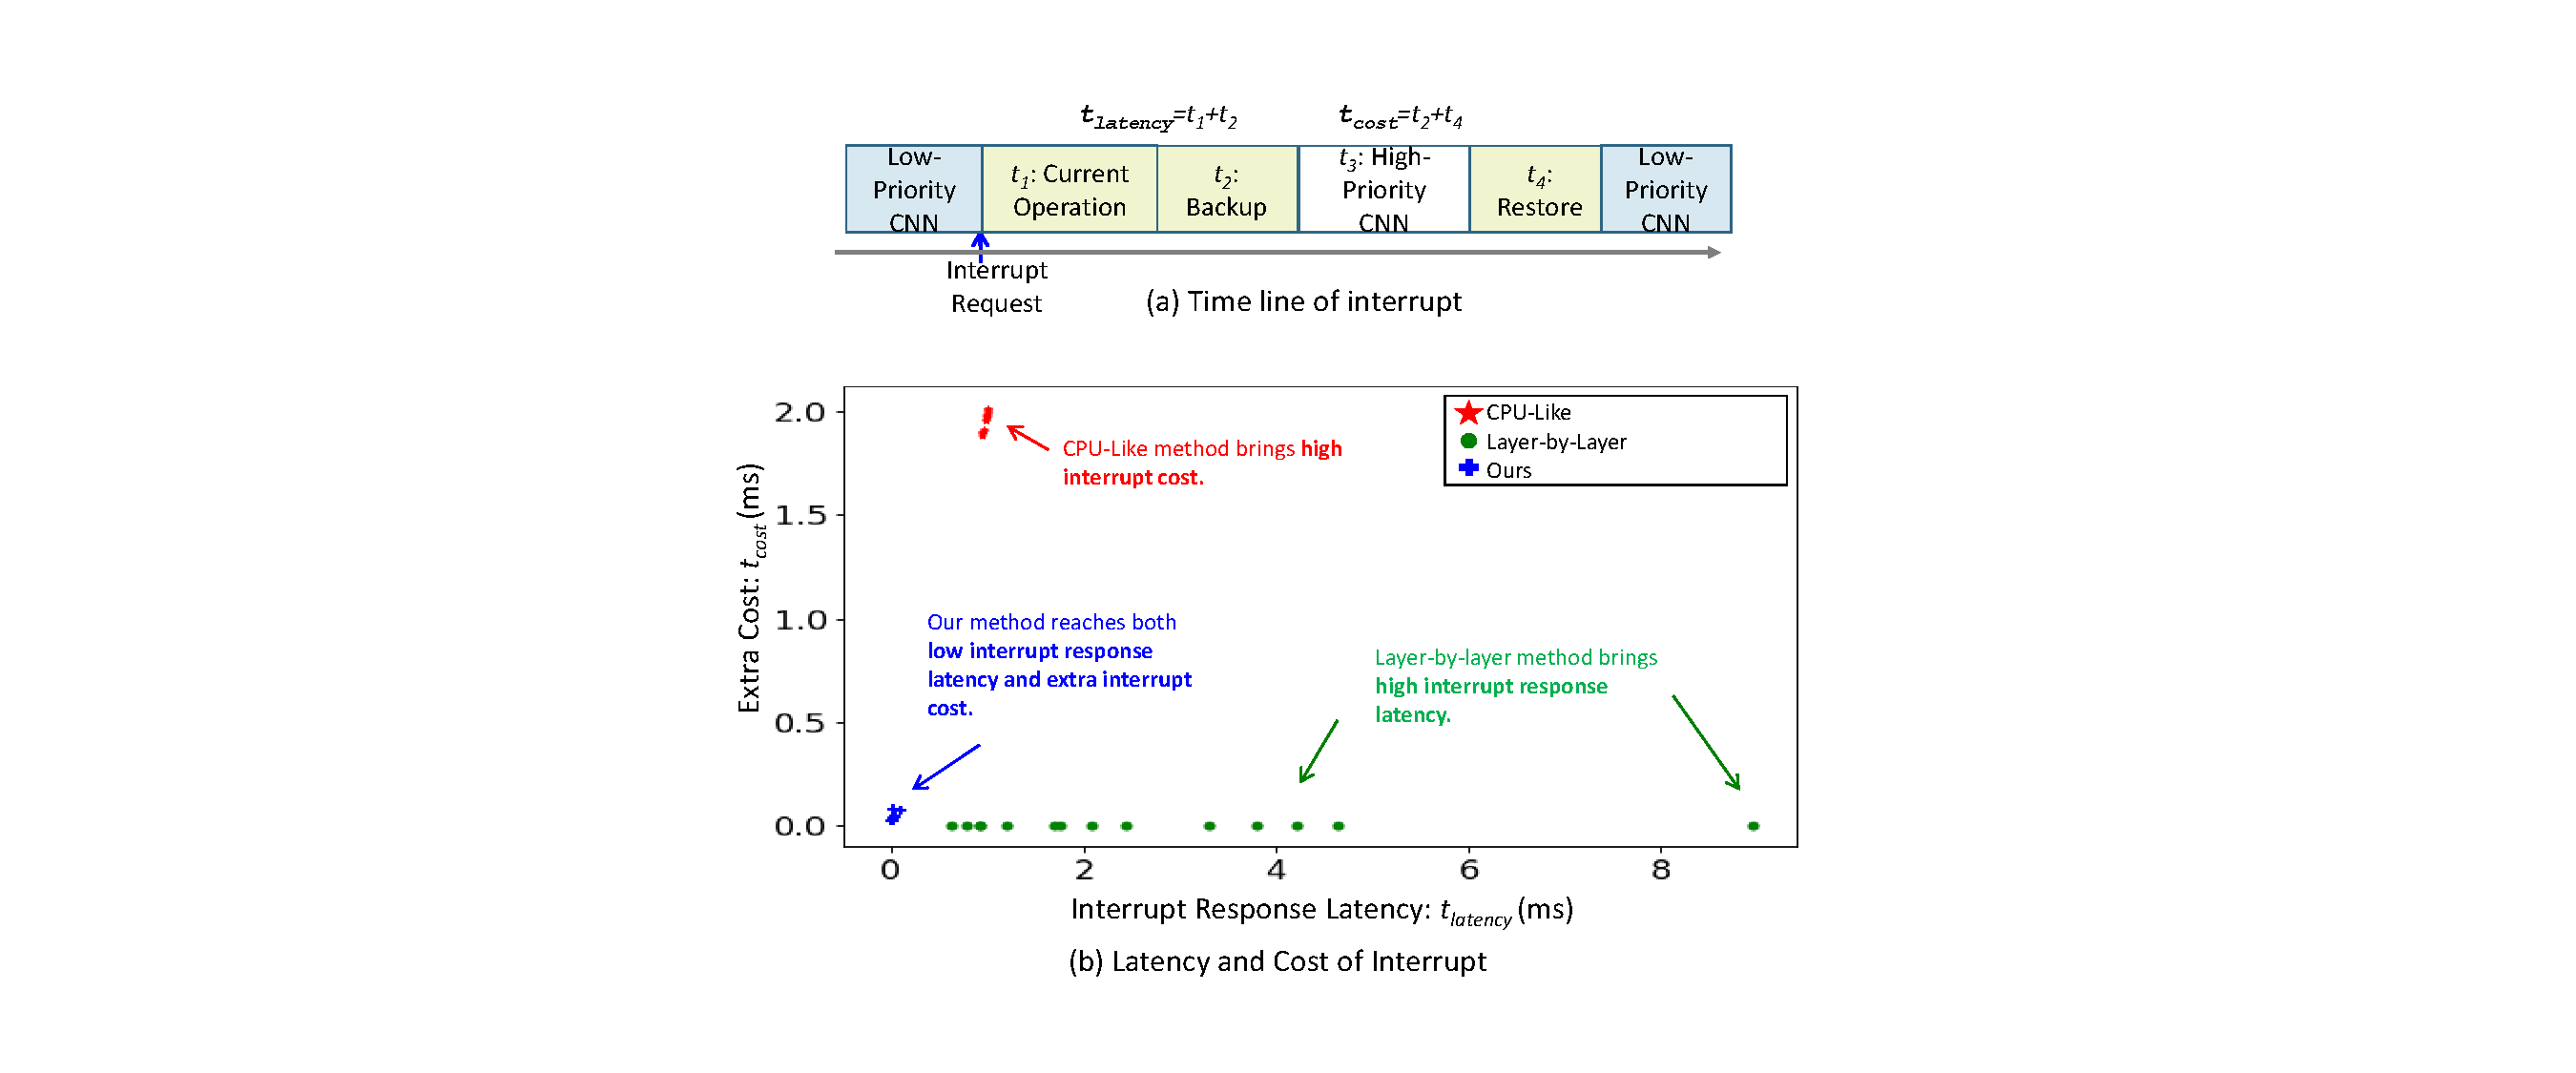
\includegraphics[width=0.99\linewidth]{fig/PRresult.pdf}
  \caption{The interrupt response latency \& extra time cost.}
  \label{fig:scatter1024}
\end{figure}
% Table generated by Excel2LaTeX from sheet 'Sheet2'
\begin{table}[t]
  \small
  \centering
  % \setlength{\abovecaptionskip}{2pt}
  \caption{The instruction number of the interruptible PR network (backbone). }
    % Table generated by Excel2LaTeX from sheet 'Sheet2'
\begin{tabular}{|c|c|c|c|c|c|}
  \hline
         & Instr.  & Instr. & Execute \\
        & Number   & volume (MB) & Time (ms) \\
  \hline
  Original ISA   &      364032      & 4.36 & 186.0 \\
  \hline
  VI-ISA   &     400243    & 4.80 & 186.4 \\
  \hline
  \end{tabular}%
  \label{tab:instrnum}%
\end{table}%



% % Table generated by Excel2LaTeX from sheet 'Sheet1'
% \begin{table}[t]
%     \centering
%     \caption{Interrupt after complete results vs Interrupt anywhere}
% % Table generated by Excel2LaTeX from sheet 'Sheet2'
% \begin{tabular}{|c|c|c|c|c|c|}
%   \hline
%   \multicolumn{1}{|c}{} &       & \multicolumn{1}{c|}{Backup } & \multicolumn{1}{c|}{Recovery} & Exe time & Performance \bigstrut[t]\\
%   \multicolumn{1}{|c}{} &       & \multicolumn{1}{c|}{data (KB)} & \multicolumn{1}{c|}{ data (KB)} & (ms)  & Reduce \bigstrut[b]\\
%   \hline
%   \multicolumn{1}{|p{3.315em}|}{Inter } & \multicolumn{1}{p{3.69em}|}{AfterSave} &       &       &       &  \bigstrut\\
%   \cline{2-6}\multicolumn{1}{|p{3.315em}|}{position 1} & Anyware &       &       &       &  \bigstrut\\
%   \hline
%   \multicolumn{1}{|p{3.315em}|}{Inter } & \multicolumn{1}{p{3.69em}|}{AfterSave} &       &       &       &  \bigstrut\\
%   \cline{2-6}\multicolumn{1}{|p{3.315em}|}{ position 2} & Anyware &       &       &       &  \bigstrut\\
%   \hline
%   \multicolumn{1}{|p{3.315em}|}{Inter } & \multicolumn{1}{p{3.69em}|}{AfterSave} &       &       &       &  \bigstrut\\
%   \cline{2-6}\multicolumn{1}{|p{3.315em}|}{position 3} & Anyware &       &       &       &  \bigstrut\\
%   \hline
%   \multicolumn{2}{|p{7.005em}|}{CPU-Like} &       &       &       &  \bigstrut\\
%   \hline
%   \multicolumn{1}{|c}{} &       & \multicolumn{1}{c|}{Instruction} & \multicolumn{1}{c|}{Latency} & Exe time & Performance \bigstrut[t]\\
%   \multicolumn{1}{|c}{} &       & \multicolumn{1}{c|}{ (KB)} & \multicolumn{1}{c|}{(ms)} & (ms)  & Reduce \bigstrut[b]\\
%   \hline
%   \multicolumn{1}{|c|}{No} & \multicolumn{1}{p{3.69em}|}{Origin} &       &       &       & 0 \bigstrut\\
%   \cline{2-6}\multicolumn{1}{|c|}{ Interrupt} & \multicolumn{1}{p{3.69em}|}{After results} &       &       &       &  \bigstrut\\
%   \cline{2-6}      & Anyware &       &       &       &  \bigstrut\\
%   \hline
%   \end{tabular}%
  
%     \label{tab:anywhere}%
%   \end{table}%



% \subsection{ **Place Recognition With the CNN accelerator }

% In this section, we evaluate the accuracy of the PR network on the CNN accelerator with fixed-point number. 

% \begin{figure}[t]
%     \centering
%     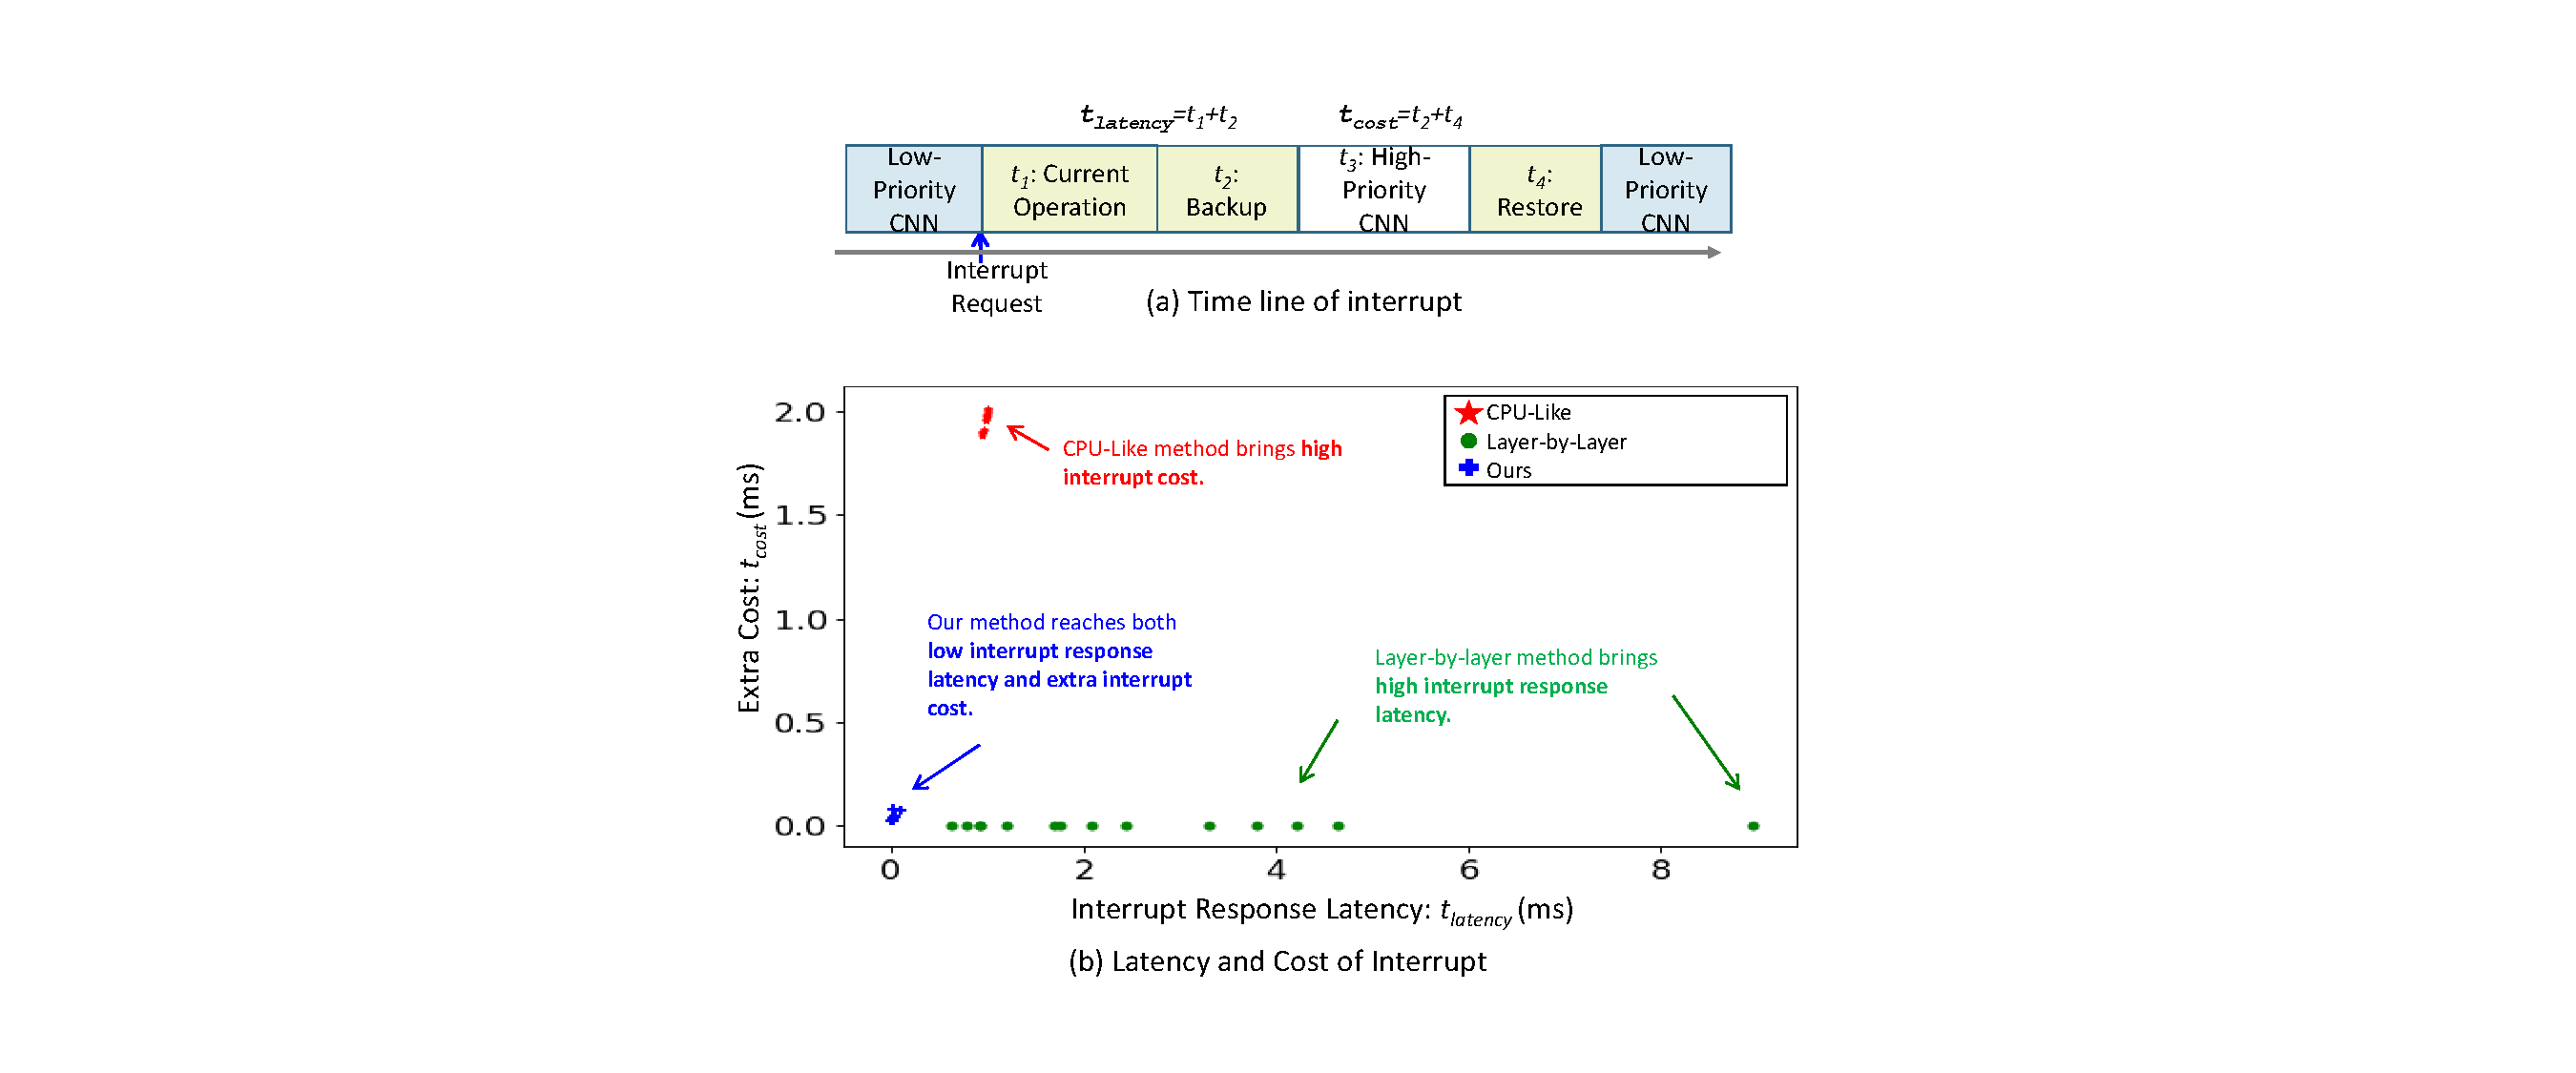
\includegraphics[width=0.8\linewidth]{fig/PRresult.pdf}
%     \caption{Precision-Recall curve on Citycenter dataset}
%     \label{fig:PRcurve}
% \end{figure}

% % We want to prove two things in our experiment. 1) The GeM network used in our work outperforms other networks such as NetVLAD. 2) The quantization of GeM CNN backbone don't bring about much drop in accuracy. 
% We test 3 networks, a) float-point GeM, b) float-point NetVLAD, c) fixed-point GeM on Citycenter dataset [??] and draw the Precision-Recall curve. The result is shown in figure \ref{fig:PRcurve}. It's clear that after quantization, the accuracy slightly reduced and still outperforms the float-point NetVLAD network  ~\cite{arandjelovic2016netvlad}, especially at higher recall, which is used in the MA-Exploration system.

% \begin{figure}[t]
%   \centering
%   \includegraphics[width=0.8\linewidth]{fig/example.eps}
%   \caption{Example of GeM performance.}
%   \label{fig:gem_exp}
% \end{figure}

% Figure \ref{fig:gem_exp} shows an example in our similation environment. Picture 1 and Picture 2 is photoed in the same place and Picture 3 is photoed in another place. The computed similarity of Picture 1 and 2 is 0.8887, apparently larger than the similarity of Picture 2 and 3 (0.8046).

% \subsubsection{efficiency}

% \begin{table}
%     \label{tab:gem_eff}
%     \centering 
%     \caption{running time comparison of each operation in PR}
%     \begin{tabular}{|c|c|c|}
% 				\hline
%               & CPU & CPU+FPGA \\
%         \hline
%            &   48 ms &   42 ms \\
% 			  \hline
%     \end{tabular}
%   \end{table}

% As illustrated in section \ref{sec:hardsoftcodesign}, we do optimization on GeM backend processing, i.e., the GeM pooling layer. We compare running time before and after optimization, and the result is shown in table \ref{tab:gem_eff}. After optimization, the total time reduces by 12.5\%.


\subsection{ FE Evaluation }

We evaluate the performance of the SuperPoint network in VO on the $TUM$ dataset ~\cite{sturm12iros}. We evaluate SuperPoint against two well-known handcrafted FE systems: SIFT ~\cite{Lowe-478} and ORB ~\cite{Mur-Artal:2017281}. 
We also evaluate the performance after optimization. 
We extract a maximum of 200 feature-points at a $480\times640$ input resolution. 
We perform nearest neighbor matching from descriptors in adjacent frames with a maximum allowable distance $d_m$. $d_m$ is not the same in three FE systems because these three descriptors are different. In PS side, we use an OpenCV implementation (solvePnP()) with all the matches to compute the transform matrix  ~\cite{LepetitMoreno-Noguer-EPnP}, and use Bundle Adjustment (BA) to optimize results  ~\cite{TriggsMclauchlan-Bundle-Adjustment}. 
% All the computation of this experiment is all done on the CPU except CNN of SuperPoint. 

Results are shown in \Cref{tab:VO}. In terms of accuracy, SuperPoint outperforms ORB and SIFT. Our optimizations, including fixed-point quantization, and post-processing acceleration, do not introduce a large loss of accuracy. 
% In terms of calculation speed, SuperPoint takes less time than Sift, and is equivalent to ORB. 
% After optimization, the running speed of SuperPoint is increased by $4\times$, making real-time processing possible.

\begin{table}[t]
  \centering
  % \setlength{\abovecaptionskip}{2pt}
  \caption{Running time comparison of each FE operation}
    \begin{threeparttable}
% Table generated by Excel2LaTeX from sheet 'Sheet2'
\begin{tabular}{|c|c|c|c|c|c|}
  \hline
             &CNN$^*$ &    Softmax &        NMS &       Rank &  Norm \\
  \hline
         CPU & \multirow{2}{*}{24ms} &      31ms &       27ms &       0.97ms &       42ms \\
  \cline{1-1} \cline{3-6}
    Ours & \multirow{2}{*}{} &    1.97ms &      0.7ms &     0.12ms &     1.44ms \\
  \hline
  \end{tabular} 
  \small
\begin{tablenotes}
   \item[*] CNN backbone runs on the accelerator.  
\end{tablenotes}
    \end{threeparttable}
  
  \label{tab:optimization}%
\end{table}%

We compare the running time of each operation in SuperPoint post-processing before and after the optimization. Results are shown in \Cref{tab:optimization}. The running time of post-processing is reduced by more than $20\times$. There is a certain gap between the experimental results of the acceleration effect and the theoretical derivation in \Cref{subsec:FEopt}. The possible reason is that the CPU needs time to schedule the FPGA accelerator.

\begin{table}[t]
  \centering
  % \setlength{\abovecaptionskip}{2pt} 
  \caption{ Accuracy and running time results on the TUM ~\cite{sturm12iros} dataset  }
  \footnotesize
  \begin{threeparttable}
% Table generated by Excel2LaTeX from sheet 'Sheet2'
\begin{tabular}{|c|c|c|c|} 
  \hline
        & RPE$^2$(m/s) & ATE$^3$(m)  & Running time(ms) \bigstrut\\
  \hline
  SIFT  ~\cite{Lowe-478}  & 0.0319  & 0.4219 & 2397  \bigstrut\\
  \hline
  ORB  ~\cite{Mur-Artal:2017281}  & 0.0577  & 0.6105 & 229  \bigstrut\\
  \hline
  Original SuperPoint  ~\cite{detone2018superpoint} & 0.0280  & 0.3671 & 259  \bigstrut\\
  \hline
  Our Fixed SuperPoint  & 0.0283  & 0.3976 & 59  \bigstrut\\
  \hline
  \end{tabular}%
  

\begin{tablenotes}
  \item[1] RPE is the mean Relative Pose Error to indicate the translational drift per second. The less, the better.
  \item[2] ATE is the root mean square Absolute Trajectory Error to indicate the translational drift of the entire trajectory. The less, the better.
\end{tablenotes}
    \end{threeparttable}
  \label{tab:VO}%
\end{table}%

% \vspace*{-2mm}
\subsection{ ROS based MR-Exploration }

The results of the Multi-Robot Exploration based on INCAME is shown in \Cref{fig:env}. The space in the AirSim~\cite{shah2018airsim} for the robots to explore is shown in \Cref{fig:env}(a). It is a simple rectangle area with four different pillars, and some chairs at the center (in the white box).  \Cref{fig:env}(b) shows how PR works for map merging. The FE and VO of each agent produce the local map and trajectory on each ZCU102 board. When the PR threads on different agents find out a similar scene, the relative pose of the two agents at the similar scene is calculated. The map and the trajectory is merged with the calculated relative pose, as shown in \Cref{fig:env}(c).

In this example, the FE and PR are both executed on the same Angel-Eye accelerator. The frequency of the input camera is 20fps, and each input frame is fed to the FE, and FE module would take up accelerator. While the CPU process VO with the feature-points from FE, the accelerator can switch to process the low-priority PR task. Because the executing time of VO varies, the time to finish a PR task is different. In this example, the time from the beginning of a PR to its end is 320$\sim$500 ms. Thus, the PR process one key frame every 7$\sim$10 input frames.

\section{Conclusion}
\label{sec:conclusion}

In this paper, we propose an interruptible CNN accelerator and a deployment framework, INCAME, for multi-robot exploration. 
With the help of virtual-instruction-based interrupt method, the CNN accelerator can switch between different CNN tasks with low interrupt response latency and low extra cost. Note that the development of CPU task scheduling evolved from single-core multi-tasking to multi-core multi-tasking. Similarly, INCAME currently focuses on interrupt support for single-core multi-tasking. We plan to investigate the multi-core multi-tasking for CNN accelerators as part of the future work.
INCAME only needs to modify the instruction fetch module to IAU in hardware. Thus, it is easy to extend to handle other instruction-driven accelerators.
Therefore, the independent software in ROS can access the accelerator without hardware resources conflicts, so that the ROS-based MR-Exploration can achieve real-time performance on embedded FPGA. In the future, more robotic algorithms, such as DOpt, Exploration and Navigation, can be implemented on hardware and included in INCAME, to gain a better energy efficiency and achieve better real-time performance.

% asWith the help of the virtual-instruction based method,

%%
%% The acknowledgments section is defined using the "acks" environment
%% (and NOT an unnumbered section). This ensures the proper
%% identification of the section in the article metadata, and the
%% consistent spelling of the heading.
% \begin{acks}
% To Robert, for the bagels and explaining CMYK and color spaces.
% \end{acks}

%%
%% The next two lines define the bibliography style to be used, and
%% the bibliography file.
\bibliographystyle{ACM-Reference-Format}
\bibliography{src/fpgaslam}

%%
%% If your work has an appendix, this is the place to put it.
% \appendix

\end{document}
\endinput
%%
%% End of file `sample-sigconf.tex'.
